%% Nirnoy's thesis, converted from the Google Docs PDF to LaTeX (compile with pdfLaTeX).
%% Figures are the original high-resolution images; Figures 1.1 and 1.2 restored.
\documentclass[11pt,letterpaper]{report}
\usepackage[margin=1in]{geometry}
\usepackage[T1]{fontenc}
\usepackage{newtxtext,newtxmath}
\usepackage{graphicx,float,longtable,array,amsmath,parskip}
\usepackage[hidelinks]{hyperref}
\usepackage{caption}
\captionsetup{font=small,labelformat=empty}
\setlength{\parskip}{0.7em}
\setlength{\parindent}{0pt}
\renewcommand{\arraystretch}{1.25}
% chapter headings in the document's style: "Chapter N" then the title, left aligned
\makeatletter
\renewcommand{\@makechapterhead}[1]{{\parindent 0pt \raggedright\normalfont\bfseries
  \large\@chapapp\space\thechapter\par\vspace{0.6em}\large #1\par\vspace{1.2em}}}
\renewcommand{\@makeschapterhead}[1]{{\parindent 0pt \raggedright\normalfont\bfseries
  \LARGE #1\par\vspace{1.2em}}}
\makeatother
\usepackage{titlesec}
\titleformat*{\section}{\normalsize\bfseries}
\titleformat*{\subsection}{\normalsize\bfseries}
\titlespacing*{\section}{0pt}{1.2em}{0.5em}
\titlespacing*{\subsection}{0pt}{1.0em}{0.4em}
\newcommand{\listitem}[1]{\par\hangindent=1.5em\hangafter=1 #1\par}
\newcommand{\bibentry}[2]{\par\hangindent=2.2em\hangafter=1 [#1]\ #2\par}

\begin{document}

\pagenumbering{gobble}
\begin{titlepage}
\centering
\vspace*{1cm}
{\LARGE\bfseries Design and Evaluation of a Drift-Aware Continuous Learning MLOps Framework for Financial Transaction Fraud Detection\par}
\vspace{2em}
by\par\vspace{1.5em}
  Mashud Hasan\\ 22299053\\[0.7em]
  Nirnoy Biswas\\ 24241185\\[0.7em]
  Md. Sabbir Hossain\\ 22299038\\[0.7em]
  Al Imran\\ 231011035\\[0.7em]
  Imtiaz Zaman Sami\\ 23101551\\[0.7em]
\vfill
A thesis submitted to the Department of Computer Science and Engineering\\ in partial fulfillment of the requirements for the degree of\\ B.Sc. in Computer Science and Engineering\par
\vspace{2.5em}
Department of Computer Science and Engineering\\ Brac University\\ [Month Year]\par
\vfill
\copyright\ 2026. Brac University\\ All rights reserved.
\end{titlepage}

\pagenumbering{roman}
\chapter*{Declaration}
\addcontentsline{toc}{chapter}{Declaration}
It is hereby declared that
\begin{enumerate}
  \item The thesis submitted is our own original work while completing degree at Brac University.
  \item The thesis does not contain material previously published or written by a third party, except where this is appropriately cited through full and accurate referencing.
  \item The thesis does not contain material which has been accepted, or submitted, for any other degree or diploma at a university or other institution.
  \item We have acknowledged all main sources of help.
\end{enumerate}

\textbf{Student's Full Name \& Signature:}\par\vspace{2.5em}
\begin{center}
\begin{tabular}{>{\centering\arraybackslash}p{0.42\textwidth}>{\centering\arraybackslash}p{0.42\textwidth}}
\rule{0.38\textwidth}{0.4pt}\newline Mashud Hasan\newline 22299053 & \rule{0.38\textwidth}{0.4pt}\newline Nirnoy Biswas\newline 24241185 \\[1.2em]
\rule{0.38\textwidth}{0.4pt}\newline Md. Sabbir Hossain\newline 22299038 & \rule{0.38\textwidth}{0.4pt}\newline Al Imran\newline 231011035 \\[1.2em]
\rule{0.38\textwidth}{0.4pt}\newline Imtiaz Zaman Sami\newline 23101551 &  \\[1.2em]
\end{tabular}
\end{center}

\chapter*{Approval}
\addcontentsline{toc}{chapter}{Approval}
The thesis titled ``Design and Evaluation of a Drift-Aware Continuous Learning MLOps Framework for Financial Transaction Fraud Detection'' submitted by
\begin{enumerate}
  \item Mashud Hasan (22299053)
  \item Nirnoy Biswas (24241185)
  \item Md. Sabbir Hossain (22299038)
  \item Al Imran (231011035)
  \item Imtiaz Zaman Sami (23101551)
\end{enumerate}
of Spring, 2026 has been accepted as satisfactory in partial fulfillment of the requirement for the degree of B.Sc. in Computer Science and Engineering in Summer 2026.

\textbf{Examining Committee:}\par\vspace{1em}
\noindent\begin{tabular}{@{}p{0.3\textwidth}p{0.65\textwidth}@{}}
\textbf{Supervisor:}\newline (Member) & \rule{0.5\textwidth}{0.4pt}\newline Md. Sabbir Ahmed\newline Senior Lecturer\newline Department of Computer Science and Engineering\newline Brac University \\[1.4em]
\textbf{Co-Supervisor:}\newline (Member) & \rule{0.5\textwidth}{0.4pt}\newline Naima Tahsin Nodi\newline Adjunct Lecturer\newline Department of Computer Science and Engineering\newline Brac University \\[1.4em]
\textbf{Thesis Coordinator:}\newline (Member) & \rule{0.5\textwidth}{0.4pt}\newline Dr. Md. Golam Rabiul Alam\newline Professor\newline Department of Computer Science and Engineering\newline Brac University \\[1.4em]
\textbf{Head of Department:}\newline (Chair) & \rule{0.5\textwidth}{0.4pt}\newline Dr. Sadia Hamid Kazi\newline Chairperson\newline Department of Computer Science and Engineering\newline Brac University \\[1.4em]
\end{tabular}

\chapter*{Abstract}
\addcontentsline{toc}{chapter}{Abstract}

Typically machine-learning models used for financial transaction fraud detection will be trained once and validated on a random subset of historical data. In production, this picture is not so: fraud patterns evolve over time (concept drift) and the actual label of a transaction is only revealed after a few weeks when a chargeback occurs (label delay). While statistical drift detectors on the input data are generally used in MLOps platforms to determine when to retrain, their abilities to signal performance of a fraud model when labels become available late were still not evaluated.

This thesis aims to design and test a drift aware continuous learning MLOps framework for fraud detection. As opposed to label-free drift alarms, the drift-aware means that the framework monitors drift based on the performance of the model on labels as they age. The framework tracks a LightGBM model on time-shifted labels, replays it model periodically with a performance safety net, automatically determines the train window, and only promotes a new model if a promotion gate ensures that the new model is at least as good as the live model on unseen data. It uses the MLflow, a FastAPI scoring service and monitoring dashboard, and is evaluated by replaying three public datasets (IEEE-CIS, Sparkov and Bank Account Fraud) as live streams with label delays ranging from 0 to 60 days and paired bootstrap confidence interval, walk-forward tuning, five training seeds, equal budget comparison and fault injection.

The PR-AUC of a static model decreased from 0.58 to 0.39 when tested on IEEE-CIS; input drift on the other hand was strong (PSI up to 4.6) on Sparkov and BAF, but did not affect the model's performance. Retraining was beneficial on all datasets, but for the IEEE-CIS dataset, the effect reduced from +0.078 to +0.010 PR-AUC as the window was changed to include up to 60 days of label delay. Drift-triggered retraining was definitely worse than scheduled retraining in 7/9 comparisons and was never better; drift-triggered retraining was equal to or better than delayed labels at an equal number of retrains. On two of the datasets, automatic window selection achieved the same best window peak value as considered, on the other, it was within 0.005 PR-AUC, and the promotion gate rejected all models that were based on corrupted data that it could see.

Financial Fraud Detection, Concept drift, label delay, continuous learning, MLOps, scheduled retraining, promotion gate, LightGBM, PR-AUC

\chapter*{Acknowledgement}
\addcontentsline{toc}{chapter}{Acknowledgement}

Firstly, we thank Allah SWT for what He has given us.

We are grateful for our supervisor, Md. Sabbir Ahmed sir and our co-supervisor Naima Tahsin Nodi ma'm for their guidance and support during this research. They offered us feedback, which helped to refine the research question and overcome the challenges we encountered while conducting research.

We are grateful to IEEE Computational Intelligence Society and Vesta Corporation for having made the IEEE-CIS Fraud Detection dataset available, the maintainers of the Sparkov credit-card dataset, and all the researchers whose articles and open-source tools have influenced this work.

\renewcommand{\contentsname}{Table of Contents}
\tableofcontents
\clearpage
\pagenumbering{arabic}

\setcounter{chapter}{0}
\chapter{Introduction}

\section*{1.1\quad Introduction}
\addcontentsline{toc}{section}{1.1\quad Introduction}

Digital payments have become the normal mode of payment for products and services . Millions of transactions are made every day through card payments, online shopping, mobile banking and cross-border e-commerce, each providing a chance for fraud. Financial crime is expected to cost more than 32 billion dollars per year to U.S. institutions alone [1].

So for banks and payment processors, identifying fraudulent transactions promptly and correctly is a financial challenge and a trust problem.

Modern fraud detection systems (FDS) rely on a combination of established business rules and machine-learning models that score each transaction and generate alerts for investigators [2], [3]. Many works have compared classifiers, ensembles and class-imbalance algorithms on public data [4], [5], [6],

[7]. Gradient boosted trees like XGBoost have been shown to be strong models for tabular fraud data [8],

[1]. But most of this work investigates the model at a single point in time: it is trained on a random sample of historical transactions and tested on another random sample from the same era.

Real systems don't work like that. The model is trained on the past and then utilised on the future. The future does not stand still. Customer shopping habits fluctuate, merchants and products change, and fraudsters adapt to any model that isn't able to catch them. The changing of the transaction-fraud relationship over time is known as concept drift [9], [10]. When concept drift occurs, a model that was correct when deployed gradually loses its accuracy, often suddenly. For example, Menezes and Filho observed that the F1-score of graph neural network fraud detectors trained on the IEEE-CIS dataset decreased up to 40\% in the weeks that followed [11].

A second challenge ignored by most drift research is that of fraud detection: the true label of a transaction is not known when the model is making the decision. A scam is usually only confirmed once the cardholder has identified it and filed a chargeback, and a legal transaction is confirmed once the dispute window has closed. Dal Pozzolo et al. term this verification delay and show that it has a major impact on how a fraud model may be updated [2]. Amekoe et al. found that it impacts the optimal learning strategies

[8]. In practice, the labels a system may learn from are typically weeks old, which means it can only realise that its performance has deteriorated long after the fact.

Machine Learning Operations (MLOps) has been developed to address precisely this type of problem: maintaining machine-learning models reliable after deployment using automated pipelines for training, versioning, monitoring and redeployment [9, 10]. Continuous training is a key MLOps approach, where models are retrained either at a fixed timetable or when a monitoring signal indicates that the data has deviated [9]. The latter is becoming increasingly preferred by recent research, where retraining is triggered when statistical drift metrics, such as the Population Stability Index (PSI) or the Kolmogorov-Smirnov (KS) test, cross a threshold [12], [13]. However, it remains an unanswered topic if triggers indeed follow the performance of a fraud model when labels arrive late. This thesis answers the question and develops a framework around the answer.

In this thesis, a drift-aware system is one which is aware of drift through its impact on the model: it tracks the performance of the deployed model on labels as they grow, and takes label-free drift measures as diagnostic information rather than a reason to retrain. The distinction is important, as the data will indicate, because drift indicators alone can both miss real degradation and raise alarms about drift that does no harm.

\section*{1.2\quad Motivation}
\addcontentsline{toc}{section}{1.2\quad Motivation}

The first reason of this work is the gap between the evaluation of fraud models in research and their implementation in practice. Many studies show near-perfect performance on public credit-card datasets utilising random train-test splits and synthetic oversampling [7].

Such results can be exaggerated if resampling is undertaken before the splitting, as shown by Dang et al.

[4]. Similarly, random split has a similar effect in time --- the model is evaluated on transactions from the same period it was trained on, thus concept drift is hidden. A fraud model to be used on future transactions should be evaluated on future transactions.

The second motivation is that the decision when to retrain a model is costly in both directions. Fraud gets through, and retraining too seldom means a worse model being used.

Frequent retraining costs computational resources and, more critically, raises the risk of deploying a faulty model, e.g. a model trained on incomplete or corrupted data.

MLOps systems consequently need a policy that decides when retraining is genuinely necessary and a safeguard that decides if a newly trained model can replace the one in service.

A third rationale is that recent work proposing drift-triggered retraining has been reviewed in a way that favours it. Shakil et al. suggested a feature-drift detector that indicates when retraining is justified, but tested on an artificial drift introduced into non-fraud datasets [12]. In a single industrial data set with induced drift, Wong and Perumal showed that an agentic, drift-triggered retraining scheduler was better than retraining once a week [13]. Yelleti retraining fraud models only when a drift detector fired, but assumes labels arrive quickly [14]. Shakil et al explicitly emphasise that statistical drift does not necessarily indicate a change in model performance [12].

Finally, our motivation comes from our own exploratory studies using IEEE-CIS dataset that already question the popular assumption. A single LightGBM model trained once lost around a third of its weekly PR-AUC in the following months, although the drift of its prediction scores was much below the usual warning level and only one of its ten most essential features drifted noticeably. On another dataset, Sparkov, we observed the opposite: a large input drift and a small accuracy degradation. Drift detectors can miss true decays and they can also raise false alarms. So a drift aware system has to be built around what drift detection can observe and what it cannot. This is the view taken by this thesis.

\section*{1.3\quad Problem definition}
\addcontentsline{toc}{section}{1.3\quad Problem definition}

We consider a fraud detection model deployed on a stream of card transactions. Each transaction needs to be assessed instantly but its fraud label is only available after a label delay of several days to many weeks. Over time, the distribution of transactions and the link between transaction attributes and fraud are changing. The operator of the system has to decide, at regular intervals, whether to retrain the model, on which data to retrain it and if the retrained model is safe to put into operation.

Existing techniques do not address numerous facets of this problem:

\listitem{1. unrealistic judgement Most fraud studies employ random splits of static data, so they cannot illustrate how performance evolves after deployment or the benefits of retraining [5], [7].}

\listitem{2. Inconsistent triggers for re-training. Label-free drift measures such as PSI and KS are routinely used to trigger retraining, yet it has not been established on real, naturally drifting data whether they match the performance of a fraud model [12], [13].}

\listitem{3. Delay of label ignored. Although verification latency is a distinguishing aspect of fraud detection [2],}

[8], most retraining research assume that labels are available instantaneously.

\listitem{4. No fair comparison of retraining policies. Retraining, scheduled and drift-triggered, is rarely compared in the same conditions, with adjusted settings, uncertainty estimates and realistic label delay.}

\listitem{5. Insecure model updates Automated retraining can be used to deploy a model trained on damaged labels or features; few frameworks verify whether their safeguards do anything to prevent such models.}

\listitem{6. Reproducibility limited. Studies using private bank data frequently include realistic operational settings}

[2], [15], [16].

To overcome these shortcomings the following research issues are posed in this thesis:

RQ1: What is the performance of a fraud detection model after deployment and does label-free drift reflect this change?

RQ2: What is the advantage of retraining and how can label delay influence that benefit?

RQ3: Is drift-triggered retraining better than scheduled retraining, where both are calibrated fairly and evaluated with realistic label delay?

RQ4: Can we design an MLOps framework on this to keep performance in a live stream and avoid incorrect models from production?

\section*{1.4\quad Purpose}
\addcontentsline{toc}{section}{1.4\quad Purpose}

The goal of this work is to develop and evaluate a drift-aware continuous learning MLOps framework for financial transaction fraud detection that can detect when a deployed model is becoming stale, determine if retraining is actually needed and deploy a better retrained model safely without retraining when not needed. The particular aims are to:

\listitem{1. To evaluate the existing literature on fraud detection, concept drift, label delay, retraining techniques and MLOps, and to identify the gaps addressed by this thesis.}

\listitem{2. To construct three public fraud datasets, IEEE-CIS, Sparkov and BAF for tight time-ordered evaluation, with no leakage from future transactions.}

\listitem{3. To quantify the degradation over time of a model trained once, and whether label-free drift measures (PSI of features and of model scores) follow that degradation.}

\listitem{4. For the simulation of retraining strategies for label delays in the range from 0 to 60 days: static model, scheduled retraining on all past data or on a sliding window, retraining triggered by drift in scores or by a decline in delayed-label performance.}

\listitem{5. Walk-forward tweaking of their parameters and repeated training seeds to compare these strategies with paired day-block bootstrap confidence intervals.}

\listitem{6. To create an MLOps framework with delayed-label monitoring, retraining policy, promotion gate, model registry, a score service, and a monitoring dashboard.}

\listitem{7. To evaluate the durability of the framework with genuine defects injected in the retraining jobs (corrupted labels, a chargeback outage and a feature unit problem).}

\listitem{8. To repeat the critical tests on the other two datasets to see if the results generalise}

\section*{1.5\quad Methodology summary}
\addcontentsline{toc}{section}{1.5\quad Methodology summary}

The workflow depicted in Figure 1.1 is used in this study. The paper opens with a survey of research on fraud detection, concept drift and MLOps which points out the shortcomings indicated in the problem statement. Then two public datasets are constructed. The IEEE-CIS, issued by IEEE Computational Intelligence Society and Vesta Corporation, contains 590,540 actual e-commerce transactions over 182 days with a 3.5\% fraud rate and has been used in recent drift and fraud research [11], [1]. Sparkov has around 1.8 million simulated card transactions over two years with 0.5\% fraud. Both are ordered by time, and used without any random shuffling. Per-card behaviour features for Sparkov are only computed from earlier transactions for each card, so that no information from the future leaks into the model.

\begin{figure}[H]
  \centering
  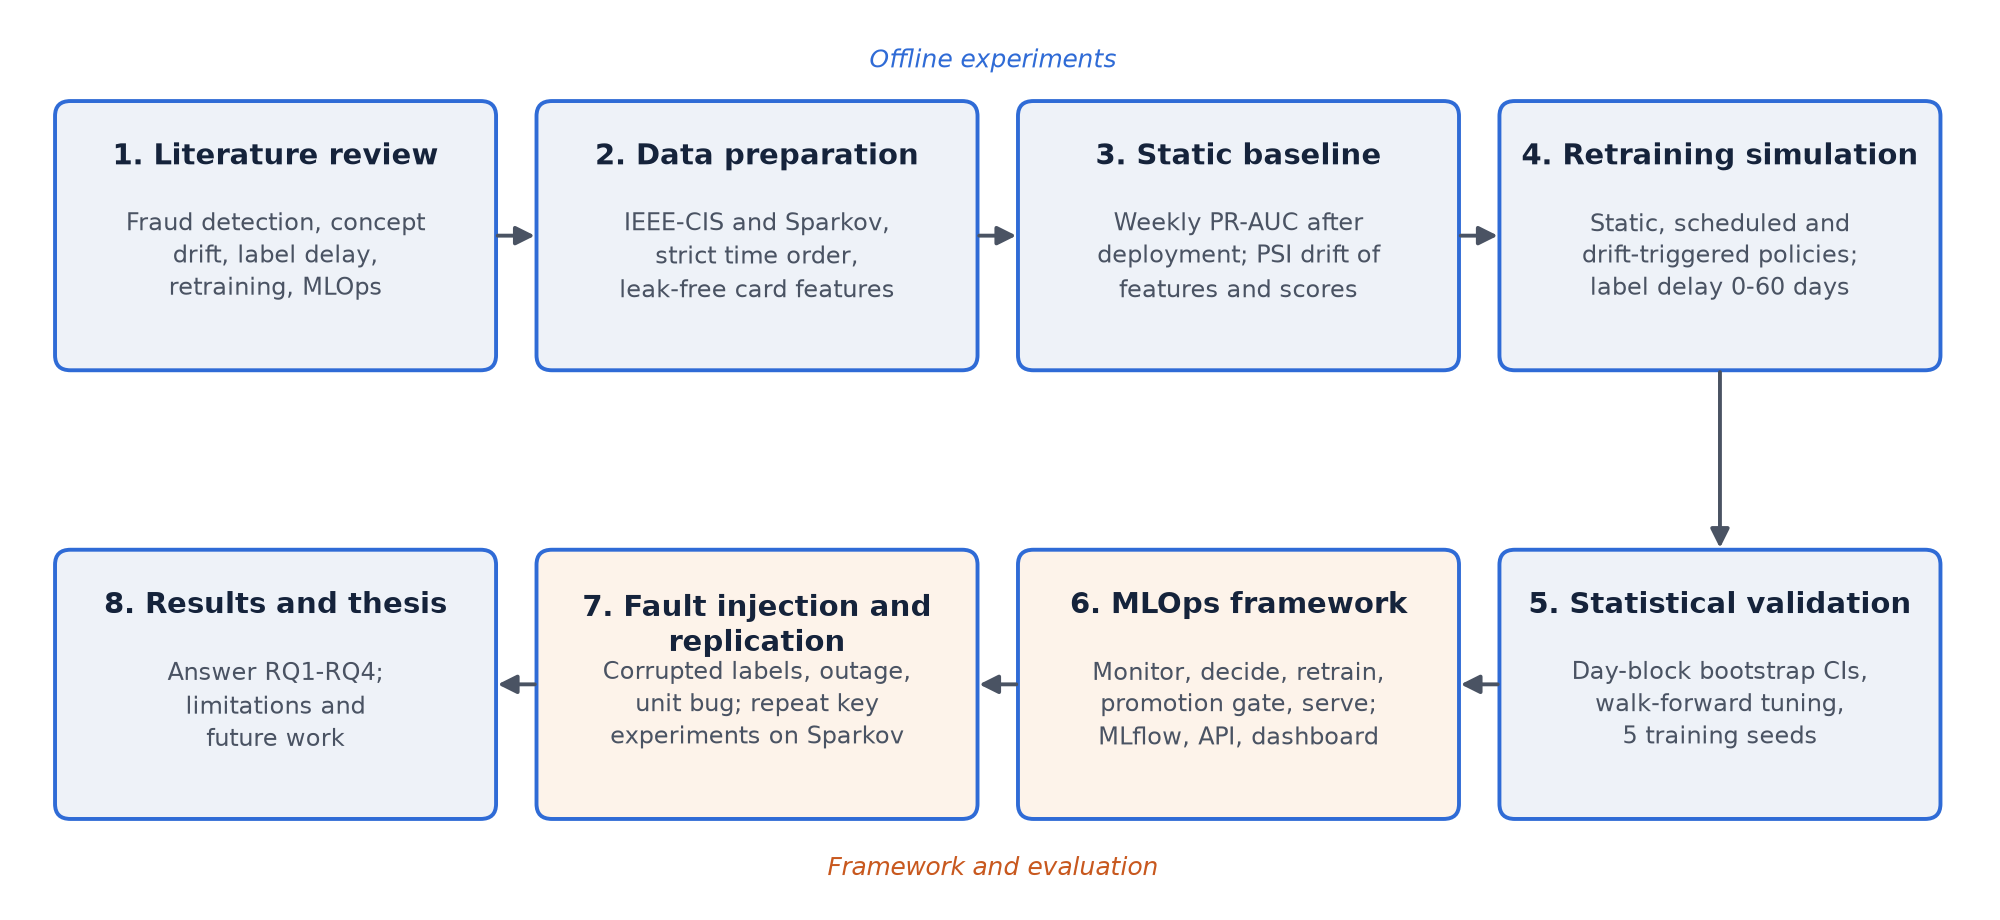
\includegraphics[width=0.95\textwidth]{figures/methodology.png}
  \caption*{Figure 1.1: Methodology of the study: from literature review and time-ordered data preparation to the retraining experiments, the framework and its evaluation}
\end{figure}

Batch-trained boosted trees are strong, frequently used models for tabular fraud data, and remain competitive with incremental learners when labels are delayed [8]. We utilise a LightGBM gradient boosted tree model throughout. In the study, they initially train a static model, and measure its weekly performance and the PSI drift of its features and scores in the following months. It then streams the latter portion of each dataset, week by week, and replicates the retraining procedures outlined in the objectives, where labels are only available after a given delay. The primary metric is PR-AUC since fraud is infrequent and precision of alerts is most important [2], scores are averaged each week thus data from multiple model versions are not combined. Uncertainty is estimated with a paired bootstrap resampling whole days, strategy parameters are modified walk-forward using only information available at the moment, and the essential comparisons are repeated with five training seeds.

The results are subsequently transformed to a workable framework, illustrated in Figure 1.2. Every week it tests the live model on labels that have become available, chooses whether to retrain, trains a new model on a sliding window of recent labelled data, and promotes it only if a promotion gate verifies that it performs at least as well as the current model on data neither has seen. Models are versioned in MLflow, delivered over a FastAPI scoring service and tracked on a monitoring dashboard, following typical MLOps practice [9]. We analyse the framework by playing the stream end to end and adding faults into selected retraining jobs to test if the promotion gate and performance safety net stop faulty models.

\begin{figure}[H]
  \centering
  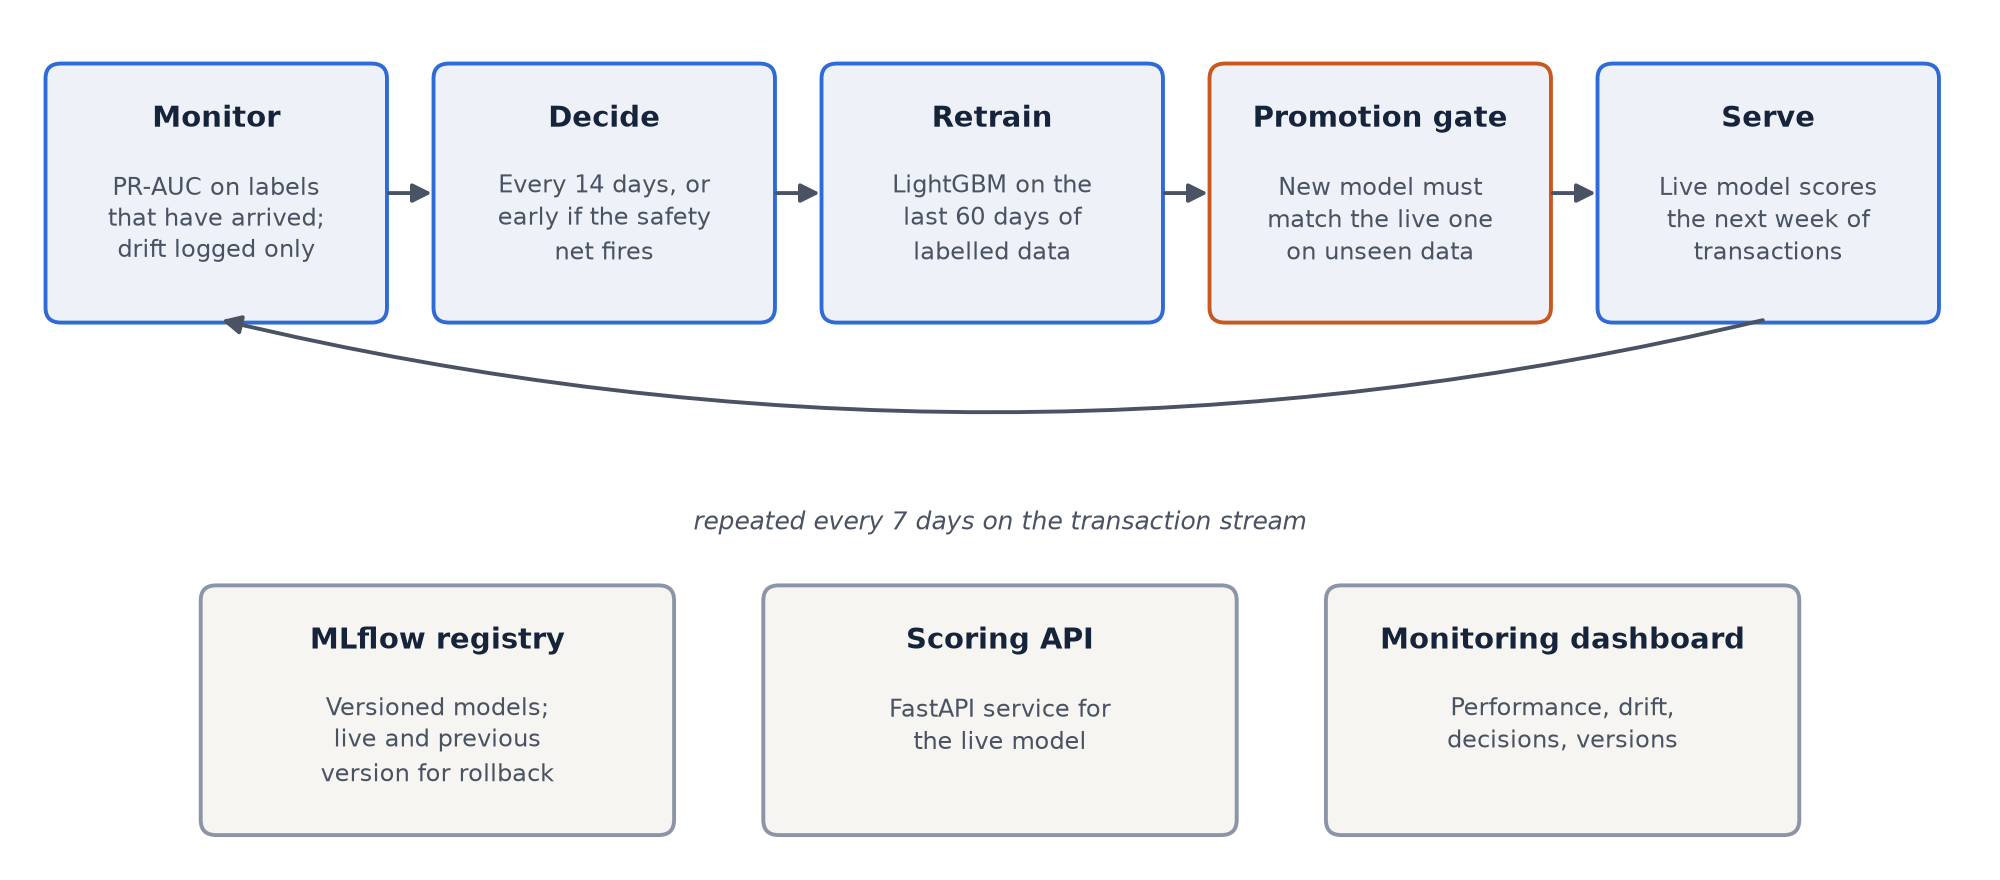
\includegraphics[width=0.95\textwidth]{figures/framework_loop.png}
  \caption*{Figure 1.2: The proposed continuous-learning loop, run every week on the transaction stream}
\end{figure}

The experiments were run on IEEE-CIS and repeated on Sparkov and on the Bank Account Fraud (BAF) dataset. They show that drift indicators can miss real degradation under delayed labels, that a fixed retraining schedule is more reliable than drift-triggered retraining when labels are delayed, also at an equal retraining budget, and that the framework reproduces the offline results when replayed. The details are given in Chapters 4 and 5.

\section*{1.6\quad Scope and Challenges}
\addcontentsline{toc}{section}{1.6\quad Scope and Challenges}

The study deals with binary fraud detection for card transactions, where each transaction is assessed as fraudulent or valid. It's about the post-deployment life of a model: how it degrades, when retraining is really required, how model upgrades can be made safe.

It is not meant to identify the best possible classifier and it does not connect to a real bank and handle real customer data. The key areas are:

\listitem{1. Fraud model evaluation on two public datasets with time-ordering}

\listitem{2. Analysis of performance degradation and label-free drift metrics after deployment.}

\listitem{3. Comparison of static, planned and drift-triggered retraining.}

\listitem{4. Statistical validation using bootstrap confidence intervals, walk-forward tuning, and repeated seeds.}

\listitem{5. MLOps framework with monitoring, retraining policy, promotion gate, model registry, score service and dashboard.}

\listitem{6. Fault injection testing of the framework's safeguards.}

\noindent\textbf{The study faces various difficulties:}

\listitem{1. Label delay: Performance can only be tested on mature labels and faults are always found late.}

\listitem{2. Class imbalance: frauds are rare (0.5\% to 3.5\% of transactions) which makes the weekly performance estimates noisy and calls for rigorous statistics.}

\listitem{3. Simulated deployment: the stream is replayed from historic data, so we don't see live latency and genuine label-feed behaviour.}

\listitem{4. Limited datasets: public fraud data with timestamps is rare; IEEE-CIS is just six months long and Sparkov is simulated.}

\listitem{5. Anonymised features: numerous IEEE-CIS features are hidden which limits the understanding of which features drift and why.}

\listitem{6. Computational cost: re-training on extended streams, multiple label delays and several policy settings takes hours of compute every experiment.}

\listitem{7. Generalisation: findings acquired with one model family and two datasets may not be generalisable to every institution or fraud type.}

Nonetheless, the study can provide practical, evidence-based advise on how to sustain fraud detection models post-deployment, and a replicable open framework that executes it.

\setcounter{chapter}{1}
\chapter{Literature Review}

\section*{2.1\quad Introduction}
\addcontentsline{toc}{section}{2.1\quad Introduction}

Fraud detection as a learning problem. Transaction fraud detection is a two

categorisation task across a constant stream of transactions. Frauds are rare, in general well

less than 5\% of transactions, the job is significantly imbalanced and accuracy is misleading

measure [5], [16]. Summary measures, like the precision and recall of the fraud class, and

PR-AUC, characterise performance more faithfully. In a functioning FDS, investigators can

only a limited amount of notifications every day, therefore the precision of the top rated alerts

matters most [2] .

Concept drift. Model drift occurs when the data you are deploying is different than the data you trained your model on and your performance declines.

[9]. no longer similar to the training data. It comes in numerous forms: notion drift, where the

relationship between features and labels changes covariate shift, where the distribution of

the input features vary; and label drift, when the frequency of the classes change [9], 2.

[10]. A change in the link between features and labels necessarily hurts a

model. A modification in inputs may or may not. Drift can also be characterised by how it takes place as shown in Figure 2.1. In quick drift the old pattern is immediately replaced; in

steady drift, old and new patterns alternate, the new one being more frequent;

in incremental drift the pattern changes gradually through intermediate states; and in recurring

past tendencies reemerge, for instance, in seasonal spending. Fraud is an antagonistic,

settinso drift is frequent, erratic and partly due to the detecting system itself [11] .

[17]. Drift detection . Drift detectors may be divided into two broad kinds. Label-free detectors differences

distribution of recent inputs or model scores relative to a reference, such as

the PSI, the KS test or Kullback-Leibler divergence [12], [13]; they are able to run right away but only observe changes in inputs or scores. The PSI is often interpreted as

steady below 0.1, mildly shifted between 0.1 and 0.25 and strongly shifted above 0.25,

and Wong and Perumal selected 0.25 as their re-training threshold [13]. Error based detectors

such as DDM, EDDM and ADWIN keep track of the model error rate and indicate drift when it

rise[14], [16]; they detect true drift but need labels arriving late to do fraud detection.

Verification delay. In a real FDS most transactions are tagged only after a delay, when

when a scam is reported or the conclusion of the dispute period; A handful of flagged transactions

get immediate feedback from investigators. Dal Pozzolo et al. formalised this as verification .

latency and the alert-feedback interaction and showed that it modifies what data a model

can learn from and when. [2] Figure 2.2 presents the result for an automated system.

At any point but not yet, the most recent weeks of transactions have already been scored

labelled. Thus performance can only be judged on older, matured transactions and a

The retrained model can only learn from data that is one label away from the present. The 2018-19 season was the longer delay he later a performance drop is noticed and the older the data a new model is trained on.

\textbf{Strategies for Adaptation.} There are many techniques to update a deployed model. Periodic or scheduled retraining rebuilds the model at defined intervals, while event-driven or triggered retraining rebuilds the model when a monitoring signal crosses a threshold [9]. The training data might be complete history (expanding window) or only recent data (sliding window) which forgets outdated patterns [2]. Incremental or online learning updates the model with every new labelled transaction and ensemble methods integrate models trained on various periods [15], [14]. The best of these depends on the speed of label arrival. With label delay, batch learning can be as good as or better than instance-incremental learning [8].

\textbf{MLOps.} MLOps is the application of software engineering practices to the machine learning lifecycle: automated training pipelines, experiment tracking, versioned model registries, continuous integration and delivery, and monitoring at production [9], [10]. Retraining can be automated using tools such as MLflow, Kubeflow and Apache Airflow, and monitoring is possible using Prometheus, Grafana and Evidently AI

[9]. Recent MLOps frameworks close the loop between monitoring and retraining for specialised domains such as phishing detection [18] and industrial prediction [13]. This is the rationale underlying the promotion gate employed in this thesis, where a frequent deployment pattern is to keep the model in service (the champion) and promote a newly trained candidate (the challenger) only if it passes an evaluation.

\textbf{Explainability under drift .} Financial authorities want model judgements to be visible and auditable, and fraud and credit models are increasingly linked with explanation approaches such as SHAP [1], [3]. These explanations are also subject to drift: if the population changes, explanations computed with an outdated reference population may be unstable or unfair [19].

\textbf{Time series evaluation.} When evaluating a drifting system, time has to be respected: models may only be trained on data collected before to the period they are evaluated on [11]. Common designs include a single chronological split, a rolling or walk-forward evaluation, and replay of a historical stream. Uncertainty estimates should resample entire blocks of time, not individual transactions, because subsequent transactions are connected.

\section*{2.2\quad Review of Related Literature}
\addcontentsline{toc}{section}{2.2\quad Review of Related Literature}

Fraud detection under drift and label delay. Dal Pozzolo et al. [2] created one of the most realistic models of credit-card fraud detection system. They partnered with an industry partner and over 75 million e-commerce transactions over three years, and explained the layers of an FDS from terminal inspections and blocking rules to the data-driven model and human investigators. They formalised the delay in verification and the interaction between an alarm and feedback from an investigator, claimed that the most important measure of performance is the precision of alerts, and recommended training separate classifiers on recent feedback from an investigator and delayed labels and aggregating their outputs. Their investigations show that emphasising recent feedback leads to more accurate alarms, and that sliding-window and ensemble methods are able to handle drift. This work provides a foundation for handling label delay as a first-class concern. The limits for this thesis are the data is private, the time of retraining is not examined and the model is not embedded into an MLOps workflow with monitoring and safe deployment.

Amekoe et al. [8] contrasted instance-incremental learning with batch learning for fraud detection with delayed labelling. Evolving streams most often favour instance-incremental algorithms, although they presume that each label is available instantly.

The authors used data of fraud detection and produced data to show that instance-incremental learning, including the Adaptive Random Forest, was not a better option than batch-trained models such as XGBoost and that batch solutions are easier to interpret as well. This finding validates the design choice of this thesis to retrain a batch model on windows of delayed labels. However the study contrasts learning paradigms, it does not study whether to retrain or how to safely install a new model.

Yelleti [14] presented ROSFD, a two stage system for online streaming fraud detection.

An initial model is generated offline using incremental learning to avoid cold start. In production, the drift detectors DDM, EDDM and ADWIN determine when the model is incrementally retrained. Across five datasets, ADWIN had the greatest performance among the detectors, and the Adaptive Random Forest earned the highest AUC on four of them, while the train-only-when-required technique considerably reduced how often the model was retrained without a big loss of AUC. The study is relevant to the subject of this thesis, as it tests re-training just when needed. It reports ROC-AUC, which is not as informative as PR-AUC for uncommon fraud and assumes labels are provided instantly, making error-based detectors seem more responsive than they actually are.

Somasundaram and Reddy [15] introduced a parallel and incremental fraud detection model called Transaction Window Bagging that integrates the techniques of parallel bagging, incremental learning, cost-sensitive learning, and weighted voting to handle both concept drift and class imbalance simultaneously. Evaluated on Brazilian bank data, it enhanced the fraud detection rate and misclassification cost vs other models. This work is significant because it considers the detection of fraud as a continuous stream and not as a static dataset. However, the data is private, the label delay is not simulated, and the influence of retraining frequency is not separated.

Al-Daoud and Abu-AlSondos [16] proposed a hybrid machine learning framework for fraud detection in the Gulf Cooperation Council banks that addresses class imbalance (SMOTEBoost and cost-sensitive learning), adversarial attacks (adversarial training and FraudGAN), concept drift (DDM and ADWIN) and explainability (SHAP, LIME and human-in-the-loop review) . In real bank transactions, it improved fraud recall from 35\% to 85\%, lowered the success rate of adversarial assaults from 35\% to 5\%, and recovered from drift in 24 hours with latency below 150 milliseconds. The study indicates that drift handling must be coordinated with the other requirements of a production fraud system. However, drift is but one component of many, the re-training policy is not compared to alternatives, and the private data inhibits replication.

Alessi and Fugini [3] proposed a real-time financial fraud detection system for transaction data streams that deals with significant class imbalance and concept drift. It employs a lightweight data stream management system for real-time feature engineering, blends deterministic rules with adaptive machine-learning models, dynamically controls the decision threshold to balance precision and recall, and compares multiple adaptive learning methodologies. It also provides an interpretability framework to translate low-level feature attributions into actionable concepts for investigators. The work provides a practical and operational view of adaptive fraud detection. However, it does not examine safeguards against inaccurate model updates or evaluate the impact of label delay on the retraining choice.

Menezes and Filho [11] examined the degradation of graph neural network fraud detectors under natural data drift. They constructed a heterogeneous knowledge graph using 284,000 IEEE-CIS transactions, trained R-GCN, HGT and HAN models on the initial 70\% and then froze the models and observed them during 50 following 12-hour intervals. All models performed worse in a volatile, non-monotonic manner; F1-score of HGT reduced from 0.747 to 0.455, while the simpler R-GCN was the most stable. They also found that the F1 score changed but the AUC kept steady, which means the distributions of scores change and fixed decision criteria become irrelevant. The study is directly relevant as it uses the same dataset and verifies that drift is a serious problem on it. However, it merely assesses degradation: no retraining method is examined, label delay is not modelled and the proposed mitigation mechanism is conceptual.

Hassan [17] put out DriftGuard-TriAudit, a concept-drift-aware continual learning methodology for financial statement fraud, which concurrently examines financial ratios, management conversation text and document structure. It incorporates modality-specific drift monitoring, reliability-weighted fusion of the three modalities, and memory-based ongoing learning.

It obtained an average precision of 0.628 on a synthetic benchmark of four temporal fraud situations, and enhanced precision compared to normal ongoing fine-tuning (0.547 vs. 0.428) with comparable AUC. The work illustrates that drift-aware continuing learning is important beyond transaction fraud, although it is about a distinct type of fraud and it is evaluated on synthetic data only.

Decision making for retraining in MLOps Shakil et al. [12] suggested a feature-drift guided methodology for retraining in MLOps. The KS statistic was paired with a confidence-based model performance indicator and a new feature-level indicator, the percent mean shift. A model was only retrained if all three indicated drift and there was enough drifted data available.

They demonstrated that applying simulated mean and variance shifts to health, loan-approval and benchmark datasets using Random Forest and SVM models showed that percent mean shift correlated more strongly with performance loss than KS statistic alone, and that the framework matched existing drift detectors while retraining less often. The study tackles only the question of when retraining is required. However, its drift is artificially created into one feature at a time, the datasets are not fraud streams, label delay is neglected and the confidence-based indicator does not measure whether predictions are true.

According to Wong and Perumal [13], a reinforcement-learning policy manages the scheduling of retraining, and data-governance controls with a composite data-quality index are included in an agentic orchestrator which is part of an AI-driven model-retraining architecture that incorporates drift detection (using the KS test and ADWIN, and PSI and Kullback-Leibler divergence for severity assessment). In a smart-manufacturing case study with injected sensor drift, the architecture improved the F1-score from 0.62 after drift to 0.93, outperforming a weekly retraining schedule while retraining only three times in six months. It gets points for the integration of retraining with data quality and for the explicit comparison to scheduled retraining. However, the evidence is restricted to one dataset with artificially induced drift, provided without confidence intervals or repeated runs, and assuming that labels are immediately available. Thus, the comparison with planned retraining is a crucial claim that is re-examined in this thesis with real fraud data and label delay.

Reda et al. [18] proposed HAMF, a hybrid MLOps framework for managing the full lifespan of adaptive phishing detection models. The 13-pipeline-stage closed loop connects data ingestion, SHAP-guided feature replacement, event-driven retraining, monitoring, fairness audits and stakeholder feedback via its microservices architecture. On three phishing datasets, it detected drift in 18 seconds, recovered an F1-score over 0.99 after drift, reduced fairness disparity by 60\%, and handled 2,300 requests per second with a p99 latency below 50 milliseconds outperforming SageMaker and Kubeflow with MLflow baselines. HAMF is a good example of a full MLOps end-to-end framework.

But phishing detection gets labels far faster than card fraud therefore its event-driven architecture cannot be immediately applied to a context with weeks of label delay.

Kodakandla [10] has proposed an end-to-end MLOps method for detecting and mitigating data drift in real-time systems like healthcare, finance and the Internet of Things, combining automated drift detection, retraining approaches and adaptive models with a focus on governance and ethics. Pulicharla [9] evaluated approaches for identifying model drift and automating retraining in ML pipelines. It covered statistical tests, drift detection algorithms, monitoring tools and retraining pipelines. They discussed the trade-off between scheduled and event-driven retraining. These studies define what an MLOps system should have for drifting data but are conceptual and do not measure which retraining policy is better for fraud detection with label delay.

Kaushik et al. [20] presented an architecture for real-time analytics by embedding machine-learning detection into streaming data pipelines built on Kafka and Flink. It features a feedback-driven module for online model updates, adaptive stream operators, hybrid edge-cloud execution, and a self-healing pipeline. In simulation, adaptive random forest with feedback had higher detection accuracy and lower false positive rate than static Isolation Forest and k-NN detectors, with reduced latency. The paper helpfully places fraud detection in a production data architecture. The evaluation is based on simulated workloads and synthetic data hence its returns

Explainability under drift . Uddin and Aziz [1] suggested a SHAP-based adaptive ensemble for explainable financial fraud detection and tested it against U.S. regulatory standards. They used the 590,540 transactions from IEEE-CIS and discovered that XGBoost with TreeExplainer yielded explanations that were almost totally stable, whereas an LSTM's explanations were weak. An adaptive ensemble achieved an AUC-ROC of 0.8837 on held-out data, and a GraphSAGE model achieved 0.9248. John [19] studied credit scoring under concept drift. SHAP explanations computed on a fixed background became unstable and unfair as populations changed. Drift-aware rebaselining of the background and online surrogate calibration improved stability and reduced disparate impact without hurting accuracy. Collectively, these papers show that explanations for a model, not only its predictions, should be preserved during drift, which is a natural extension of the framework in this thesis.

Static fraud classification. There is a huge body of work devoted to maximising performance on a static dataset. Mienye and Sun [7] developed a deep-learning ensemble of LSTM and GRU base learners, a multilayer perceptron meta-learner with SMOTE-ENN resampling and reported sensitivity of 1.000 and specificity of 0.997. Sohony et al. [6] used an ensemble of random forests and feed-forward neural networks to optimise fraud recall vs false alarms. Abd El-Naby et al. [5] used SMOTE, Borderline-SMOTE, ADASYN and SMOTETomek balancing techniques with classical classifiers and obtained good accuracy after balancing. Dang et al. [4] investigated resampling approaches, classical models and deep reinforcement learning and found that resampling before the train-test split can make results look significantly better than they are. These studies build powerful classifiers and thorough imbalance handling, but use random splits of static data therefore do not demonstrate how the models will perform after deployment.

\section*{2.3\quad Summary of the Main Findings}
\addcontentsline{toc}{section}{2.3\quad Summary of the Main Findings}

There is consensus in the literature that concept drift is a real and major problem for fraud detection.

Static models degrade after deployment, often sharply and irregularly [11], [2]. Therefore, fraud detection systems must be able to update their models over time. Sliding windows, incremental learning, ensembles and drift-triggered retraining have been proposed [2, 15, 14, 16, 3].

Delay to label is a key characteristic of fraud detection although it is never studied. Its importance was demonstrated by Dal Pozzolo et al. and Amekoe et al. [2], [8], but the majority of retraining frameworks are based on the assumption that labels are readily available [12], [13], [14], [20]. Error-based drift detectors need labels, therefore label delay restricts how fast any performance-based trigger may react.

Recent MLOps research favours retraining based on drift detection, and has shown that it beats or is comparable to scheduled retraining with less retrains [12], [13], [14]. These assertions are based on artificially produced drift, single datasets, non-fraud domains or instantaneous labelling. At the same time statistical drift does not have to mean performance drop [12]. Thus, the question remains open whether drift-triggered retraining is preferable for fraud detection in realistic situations.

Another gap is the practice of evaluation. Many fraud studies show very high results on random splits of static data [7], [5], which tell little about performance after deployment.

Only a few research employ time ordered evaluation, confidence intervals, fair tuning of competing methods or repeated runs, and studies with realistic streams frequently use private data which cannot be duplicated [2], [15], [16].

Retrained models are also infrequently deployed safely. MLOps frameworks close the loop between monitoring and retraining [18], [10] and some compare a new model with the current one [13]. However, we identified no fraud detection study testing whether such measures genuinely prohibit models trained on corrupted labels or features. Finally, drift also undermines stability of explanations [19], [1], which is important for regulated monetary systems.

These results motivate the proposal of a drift-aware continuous learning MLOps framework for financial transaction fraud detection that: (1) is evaluated on public data in strict time order, with confidence intervals, walk-forward tuning and repeated seeds; (2) models label delay explicitly and measures its limitation of the benefit of retraining; (3) compares scheduled and drift-triggered retraining fairly and retrains only when evidence shows it is necessary; (4) monitors performance on delayed labels instead of relying only on label-free drift signals; (5) protects production with a promotion gate and a performance safety net, tested by fault injection; and (6) is released as reproducible open-source code with a second dataset for replication. The next guy

\setcounter{chapter}{3}
\chapter{Methodology and Design}

\section*{4.1\quad Design Process}
\addcontentsline{toc}{section}{4.1\quad Design Process}

The study is performed by following the design process shown in Figure 4.1: explore experiments that entail monitoring the behaviour of the deployed fraud model under drift and label delay, construct a framework around this experiments and evaluate this framework using three data sets.

\begin{figure}[H]
  \centering
  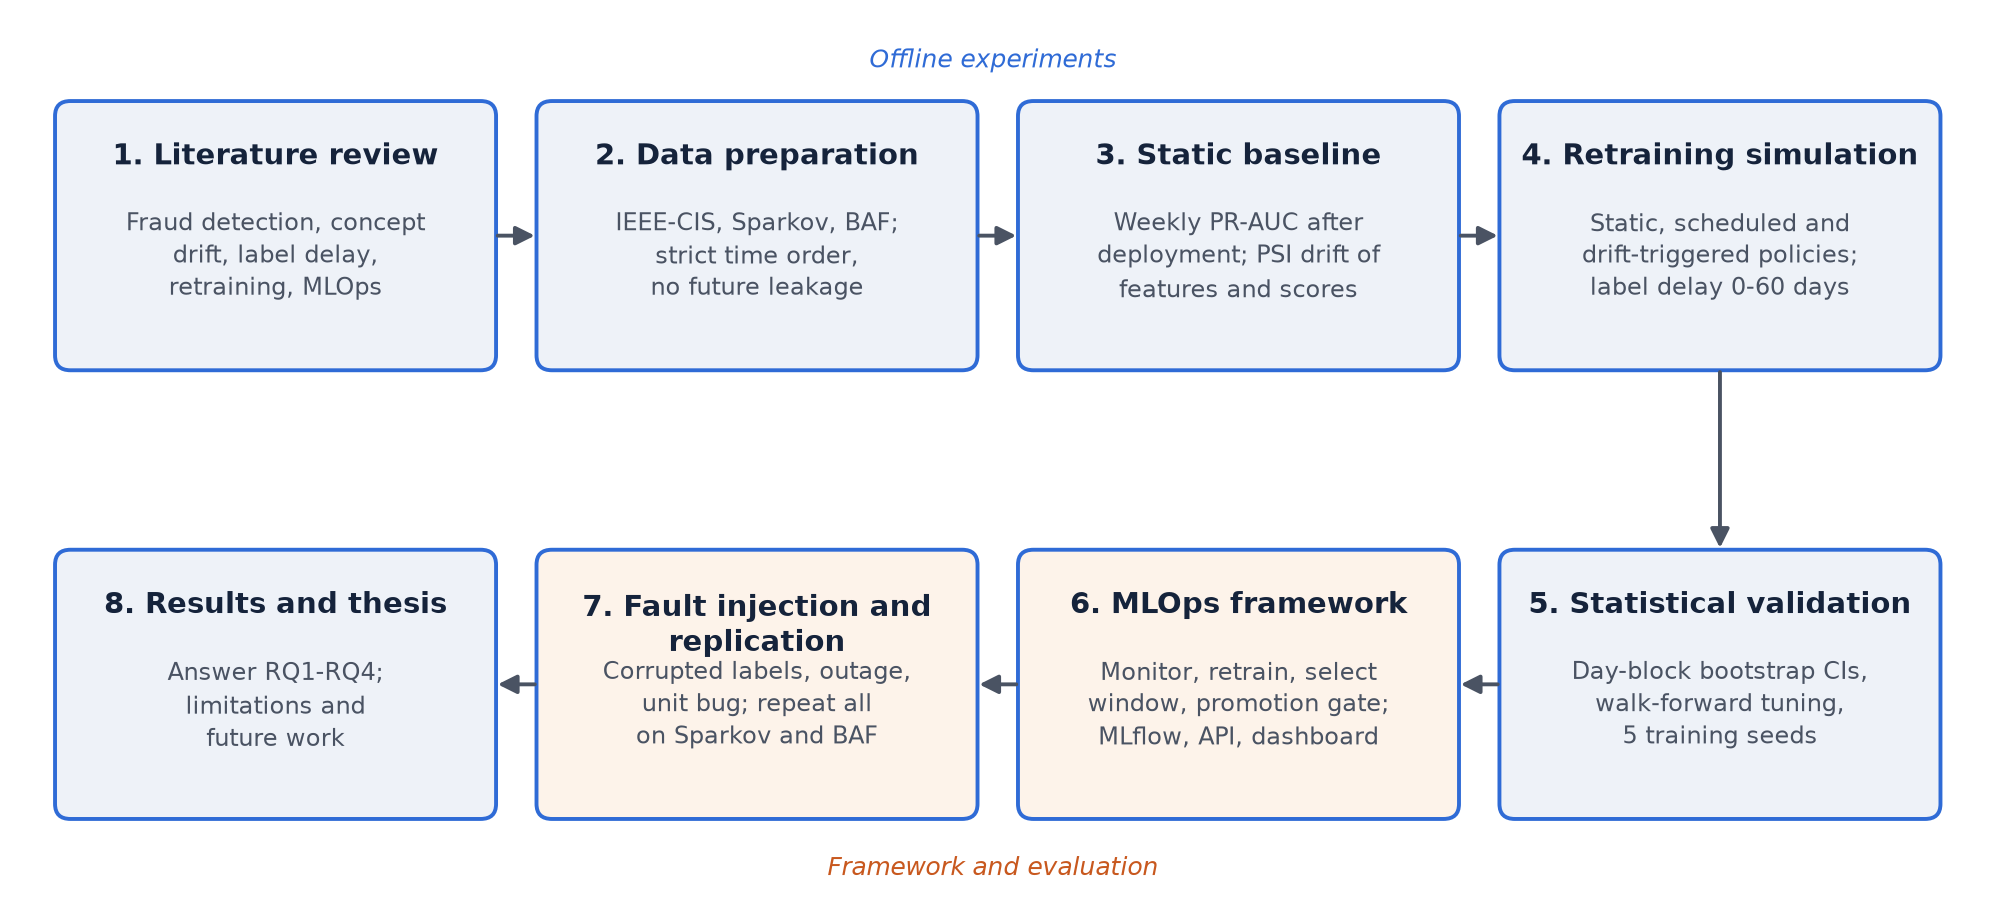
\includegraphics[width=0.95\textwidth]{figures/methodology_3ds.png}
  \caption*{Figure 4.1: Methodology overview: the experiments on three datasets, the framework and its evaluation}
\end{figure}

\subsection*{4.1.1\quad Research Design}
\addcontentsline{toc}{subsection}{4.1.1\quad Research Design}

This paper presents empirical, simulation-based analysis and then the design and evaluation of a software framework. As shown in Chapter 2, drift induced retraining depends mostly on artificial drift, instantaneous labels and datasets [1] [2] [3]. We first study the behaviour of a deployed model and the optimal retraining strategy under label delay on public fraud data with natural drift (research questions RQ1 to RQ3), and then build the framework around it and evaluate it (RQ4). Figure 4.2. presents the following steps of the study:

\begin{figure}[H]
  \centering
  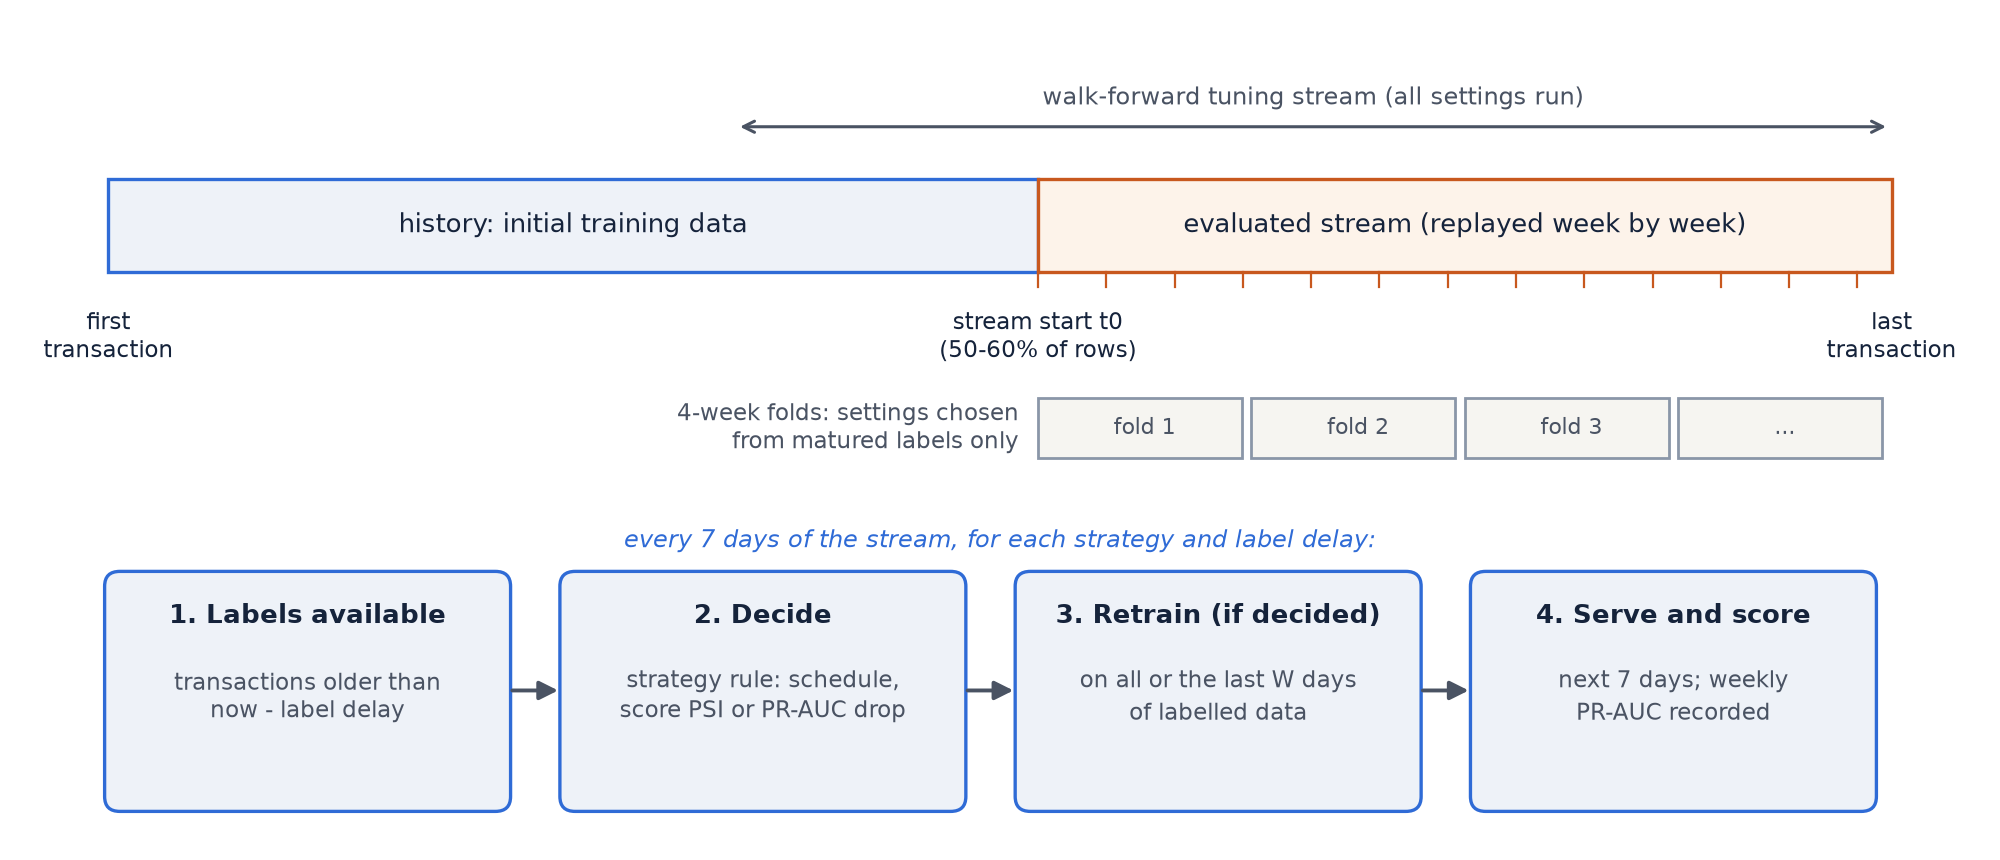
\includegraphics[width=0.95\textwidth]{figures/protocol.png}
  \caption*{Figure 4.2: Evaluation protocol: each dataset is split in time into a history and a stream that is replayed week by week; settings are tuned walk-forward in 4-week folds}
\end{figure}

Each experiment follows three principles. We first respect time, i.e. a model is only trained on transactions that happened and whose labels could be retrieved before the period it is assessed on [4]. Second, the deployment is simulated not imagined: each dataset is played as a stream one week at a time and the label delay applied is explicit as described by [5] Dal Pozzolo et al. Third, differences have to be robust to uncertainty: differences are reported with a confidence interval, the parameters of competing strategies are chosen in the same way and the major results are reproduced with numerous training seeds and with a second data set.

The rest of this section presents the simulated deployment under label delay (Section 4.1.2), the retraining strategies (Section 4.1.3), the drift and performance measures (Section 4.1.4), the statistical validation (Section 4.1.5) and the evaluation of the framework including fault injection (Section 4.1.6). The model is presented in Section 4.2, the framework in Sections 4.3 and 4.4, the data and the project plan in Section 4.5, and the outcomes in Section 4.6 the implementation.

\subsection*{4.1.2\quad Label Delay: Simulated Deployment}
\addcontentsline{toc}{subsection}{4.1.2\quad Label Delay: Simulated Deployment}

Stream is played in 7 day intervals starting with start of stream to end of data. over each phase three activities are done: the strategy defines which labels are available, and in case a retraining is needed a new model is trained and directly applied to replace the previous one; and the current model scores the transactions over the next seven days. Scores for each week are saved, together with the version of the model that generated them. The transactions would be streamed into production, similarly to the real-time pipelines of Kaushik et al. [6] over a streaming infrastructure such as Kafka or Flink. The replay of recorded data would make every experiment exactly repeatable.

We model the time delay between a transaction and the use of its label as a fixed delay, $d$ days. The labelled data accessible for monitoring and training is given by, at time $t$,
\begin{equation*}
  \mathcal{L}(t) = \{\, x_j : t_j \le t - d \,\} \tag{4.1}
\end{equation*}
where $t_j$ is the time of transaction $x_j$. The first model is trained at the beginning of the stream and is taught by the same rule, so it does not see any label that it might not have had. We consider delays of 0, 15, 30 and 60 days. The value of delay equal to 0 is commonly assumed in majority of the retraining research [3]

The amount of time a cardholder takes to notice a fraudulent charge and dispute it is 30 to 60 days [2]; [5]. Not all Investigator feedback for some alerted transactions is modelled: all labels arrive with the same delay, which is smaller in a real system [5]. This is a slightly bad background for the performance based triggers which are discussed.

\subsection*{4.1.3\quad Retraining Strategies}
\addcontentsline{toc}{subsection}{4.1.3\quad Retraining Strategies}

Five strategies are compared with the possibilities presented in Section 2.1 [7], [5]. These are summarised in Table 4.1.

The table below presents the retraining strategies that were evaluated in the simulation (default parameters).

\begin{center}\small Table 4.1: Retraining strategies compared in the simulation (default settings)\end{center}
\vspace{-1.2em}

{\small
\begin{longtable}{|>{\raggedright\arraybackslash}p{0.17\textwidth}|>{\raggedright\arraybackslash}p{0.29\textwidth}|>{\raggedright\arraybackslash}p{0.21\textwidth}|>{\raggedright\arraybackslash}p{0.17\textwidth}|}
\hline
Strategy & When it retrains & Training data & Needs labels to decide? \\ \hline
Static & Never & History before the stream & - \\ \hline
Periodic expanding & Every 14 days & All labelled data so far & No \\ \hline
Periodic sliding & Every 14 days & Labelled data of the last 60 days & No \\ \hline
Drift: score PSI & PSI of the model's scores over the last week, against its validation scores, exceeds 0.1 (at least 14 days apart) & All labelled data so far & No \\ \hline
Drift: performance & PR-AUC on newly matured labels falls more than 15\% below the reference (Equation 4.2; at least 14 days apart) & All labelled data so far (or the last 60 days in tuned variants) & Yes (delayed) \\ \hline
\end{longtable}
}

The base is the static model trained at the beginning of the stream, which doesn't change. The difference between the two periodic techniques is that the expanding window contains all labelled data collected while the sliding window only contains the previous 60 days and discards old patterns.

A classic label-free drift trigger is the score-PSI method [1], [2]. The distribution of scores it has produced in the last week is compared with the distribution of scores it has produced on its own validation data (PSI from section 4.1.4) and if the PSI is above the standard threshold of 0.1 it is considered to be displaced and is retrained. It is label-free and may therefore respond immediately.

The performance method is a simple error based trigger in the sense of DDM and ADWIN [3] [8] adapted for delayed labels. It computes the PR-AUC of the model on transactions with labels from the past 14 days not included in the model training, if there are at least 30 frauds in these transactions at each phase. It retrains when
\begin{equation*}
  \mathrm{AP}_{\mathrm{live}}(t) < (1 - \tau)\, \mathrm{AP}_{\mathrm{ref}} \tag{4.2}
\end{equation*}
where $\mathrm{AP}_{\mathrm{live}}(t)$ is that live PR-AUC, $\tau$ is the tolerance (0.15 by default), and $\mathrm{AP}_{\mathrm{ref}}$ is either a model's validation PR-AUC, or the initial live measurement. Both drift techniques include a minimum of 14 days between retrains, to avoid a series of retrains owing to one drift occurrence.

The identical data, model settings and random seed are utilised for each strategy and each label delay, the only difference between the runs is the decision of whether or not to retrain and the training window. The large number of runs is because models trained on the same windows are cached and reused across strategies and because equivalent decisions lead to equivalent models.

\subsection*{4.1.4\quad Drift and Performance Measures}
\addcontentsline{toc}{subsection}{4.1.4\quad Drift and Performance Measures}

Population Stability Index The PSI measures drift in a feature or in the scores of the model by comparing a current distribution with a reference distribution [2]:
\begin{equation*}
  \mathrm{PSI} = \sum_{i=1}^{B} (c_i - r_i)\,\ln\frac{c_i}{r_i} \tag{4.3}
\end{equation*}
with reference values binned into $B = 10$ bins at the deciles of the values. $r_i$ and $c_i$ are shares of the reference and current values in bin $i$. Shares are floored at $10^{-6}$ to avoid division by zero. Missing values are binned in their own bin. A PSI less than 0.1 is usually regarded steady, 0.1 to 0.25 is considered a moderate change, and greater than 0.25 is considered a major change. The PSI is determined for the 10 most relevant features of the static model (by total gain) and for the scores, in each time bin compared to the training period.

PR AUC. Fraud is exceedingly rare and investigators can only investigate the highest scoring alerts the main criterion is the area under the accuracy recall curve as determined by average precision [5]:
\begin{equation*}
  \mathrm{AP} = \sum_{n} (R_n - R_{n-1})\,P_n \tag{4.4}
\end{equation*}
where $P_n$ and $R_n$ are the precision and recall at the $n$-th threshold of the ranked scores. The high number of genuine transactions does not inflate the PR-AUC. It also does not have the ROC-AUC bias on the cleanliness of the top of the alert list [9]. Note that the PR-AUC of a no-skill model is equal to the fraud rate.

Average PR AUC per week. Each week a different version of the model is used to score, and the scores of different versions are not normalised to each other. A single PR-AUC computed over all weeks would blend such measures and often penalise training tactics even when their own models ranked transactions well. Therefore, we compute PR-AUC for each week $w$ of the stream independently, then average PR-AUC over the $W$ weeks:
\begin{equation*}
  \overline{\mathrm{AP}} = \frac{1}{W} \sum_{w=1}^{W} \mathrm{AP}_w \tag{4.5}
\end{equation*}
If no fraud is found in one week, that week is skipped. Secondary measurements are minimum weekly PR-AUC, minimum number of retrains and F1-score at each model's own threshold.

\subsection*{4.1.5\quad Statistical Validation}
\addcontentsline{toc}{subsection}{4.1.5\quad Statistical Validation}

Day-block bootstrap, paired. Weekly PR-AUC is noisy for weeks with only a few hundred frauds, because there is correlation between subsequent transactions. The confidence intervals are generated this way because bootstrap samples days, not individual trades. Days in each week are sampled with replacement and the mean weekly PR-AUC is re-computed in each week. For each strategy, the same resampled days are utilised, so that the differences across methods are paired and a lot of the same noise removed. The resampling is 500 and 95 \% percentile intervals are provided. If an interval does not include 0, the difference is regarded dependable.

Forward walk tuning. All techniques should have good settings that cannot be determined from the data used for the evaluation. All 190 configurations of Table 4.2 are performed on a tuning stream that starts at 35\% of the rows, earlier than the stream analysed. The stream under scrutiny is divided into four week blocks which are termed folds. Each fold, each family (static, scheduling, drift performance) selects the best scored one to start the fold.

\begin{equation*}
  J(c) = \overline{\mathrm{AP}}(c) - \kappa \cdot \frac{N_{\mathrm{retrain}}(c)}{\text{number of 4-week periods}} \tag{4.6}
\end{equation*}
$\kappa = 0.002$ is a low cost per retrain, which breaks ties in favour of simpler configurations (as only computed on weeks whose labels have matured by the start of the week of the fold; i.e., on information that would really have been available). The results of the selected configuration on the fold are then recorded down and the same configuration is picked for the following fold. The result is a reasonable approximation of the performance of each family if an operator had the knowledge available at the time to tune the family to that information.

\begin{center}\small Table 4.2: Settings searched by walk-forward tuning (190 configurations)\end{center}
\vspace{-1.2em}

{\small
\begin{longtable}{|>{\raggedright\arraybackslash}p{0.293\textwidth}|>{\raggedright\arraybackslash}p{0.293\textwidth}|>{\raggedright\arraybackslash}p{0.293\textwidth}|}
\hline
Family & Setting Searched & Configurations \\ \hline
Static & - & 1 \\ \hline
Schedule & Expanding window, period 7, 14 or 28 days; sliding window, period 7, 14 or 28 days and window 30 or 60 days & 9 \\ \hline
Drift:performance & Tolerance 0.05, 0.1, 0.15, 0.2 or 0.3; monitoring window 7, 14 or 28 days; minimum gap 7, 14 or 28 days; reference = validation PR-AUC or first live measurement; training data = all or last 60 days & 180 \\ \hline
\end{longtable}
}

The bootstrap merely takes into account the uncertainty of the evaluation sample. Also, LightGBM training is random, using row subsampling and feature subsampling. The important runs are then repeated with five different random number seed (42, 1, 2, 3 and 4) with the two label delays (0 days and 30 days). For each comparison the mean and range of differences and number of random number seeds for which the difference is of the same sign is reported.

\textbf{Repetition.} Finally the whole process from the static baseline, to the delay sweep, walk forward tuning, seeds and the replay of the framework is replayed with the same scripts and settings on Sparkov and BAF. If the result is not found on the other datasets but is found on IEEE-CIS, the discovery is described as dataset-specific.

\subsection*{4.1.6\quad Framework Evaluation and Fault Injection}
\addcontentsline{toc}{subsection}{4.1.6\quad Framework Evaluation and Fault Injection}

The system is tested by applying it to the evaluation stream for each of the datasets as if it were live, with a label delay of 30 days. Uses the same data store and the same code and MLflow model registry as a deployment. And contrasted to the static model, the offline simulation of the same policy that ensures that the framework reproduces the findings from the experiments. The framework is rerun on each dataset with four versions on the same machine: static model, 60 day window, entire history, and automatic selection to determine window selection. The four replays share a set of trained models, so given the same training data there will be only one training of the model, and the only difference in the four replays is their decisions.

Now you have an autonomous retraining pipeline and then it can eventually train on faulty data. To validate that the safeguards in the framework prohibit such models, we introduce the errors in Table 4.3 in selected retraining jobs of the replay (by default the second and fourth occur in the schedule). The faults simulate typical pipeline failures: misaligned join, chargeback feed outage, and unit change during training and serving. In the first three, only the data that the training job consumes is corrupted. The production feature path and the label-store are left correct. The fourth is the gate failing on purpose, and corrupting the label store the gate reads. This can be used to determine if the safety net keeps the harm restricted.

\begin{center}\small Table 4.3: Faults injected into retraining jobs to test the safeguards\end{center}
\vspace{-1.2em}

{\small
\begin{longtable}{|>{\raggedright\arraybackslash}p{0.293\textwidth}|>{\raggedright\arraybackslash}p{0.293\textwidth}|>{\raggedright\arraybackslash}p{0.293\textwidth}|}
\hline
Fault & What goes Wrong & Real-world cause \\ \hline
Label shuffle & Labels are permuted within the training window, so they no longer match their transactions & A misaligned join in the training job \\ \hline
Label loss & 80\% of frauds in the training window are recorded as legitimate & An outage of the chargeback feed \\ \hline
Feature unit bug & The five most important numeric features of the live model are multiplied by 100 in training only & A unit change (e.g. cents and dollars) between training and serving \\ \hline
Upstream label shuffle & The label store itself is corrupted, so the promotion gate also reads wrong labels & Corruption at the source; a known blind spot \\ \hline
\end{longtable}
}

Each fault scenario is executed twice: with and without the promotion gate and is compared with a clean replay. A safeguard is effective when the performance of a run with the fault and the safeguard remains close to the performance of a "clean" run, and the performance of a run without the safeguard deteriorates. Each scenario creates its own MLflow store and thus does not impact the main registry.

\section*{4.2\quad Design (Model) Specification}
\addcontentsline{toc}{section}{4.2\quad Design (Model) Specification}

In this section, the Fraud Detection model adopted in this study is mentioned and the components of the drift aware Continuous Learning framework are described.

\subsection*{4.2.1\quad Fraud Detection Model}
\addcontentsline{toc}{subsection}{4.2.1\quad Fraud Detection Model}

We use LightGBM, a gradient boosted decision tree (GBDT) toolkit, and perform tests with the settings of Table 4.4. Gradient boosted trees are stable and popular models for tabular fraud data [10, 11], native to missing values and categorical characteristics, and can be retrained hundreds of times without taking too much time. Additionally, Amekoe et al. noticed that the batch-trained boosted trees compete with incremental learners in the presence of late arriving labels, like in our work [11]. The goal is not to get the best possible classifier, as in many static research [12] [9] [13] but to set one strong and realistic model and focus on the difference between different retraining procedures. Not resampled (like SMOTE) as this can make evaluation harder [14], class imbalance managed by weighting the fraud class, also utilised by Somasundaram and Reddy in case of imbalance in a drifting fraud stream [15].

The model architecture is depicted in figure 4.3. Each transaction is characterised by its features, 431 in the IEEE-CIS, 16 in Sparkov and 29 in BAF. LightGBM builds an ensemble of choice trees sequentially - each decision tree can have 256 leaves, and each tree will be fit on the residuals of previous ones. Training will stop if the validation AUC does not improve in 100 rounds (or 2000 trees). The score F (x) is the sum of the outputs from all trees . For a new transaction , a sigmoid function converts the score to a fraud . Probability value ranging from 0 to 1 . When the probability value is greater than a decision threshold as defined below, the transaction is recognised as fraud.

\begin{figure}[H]
  \centering
  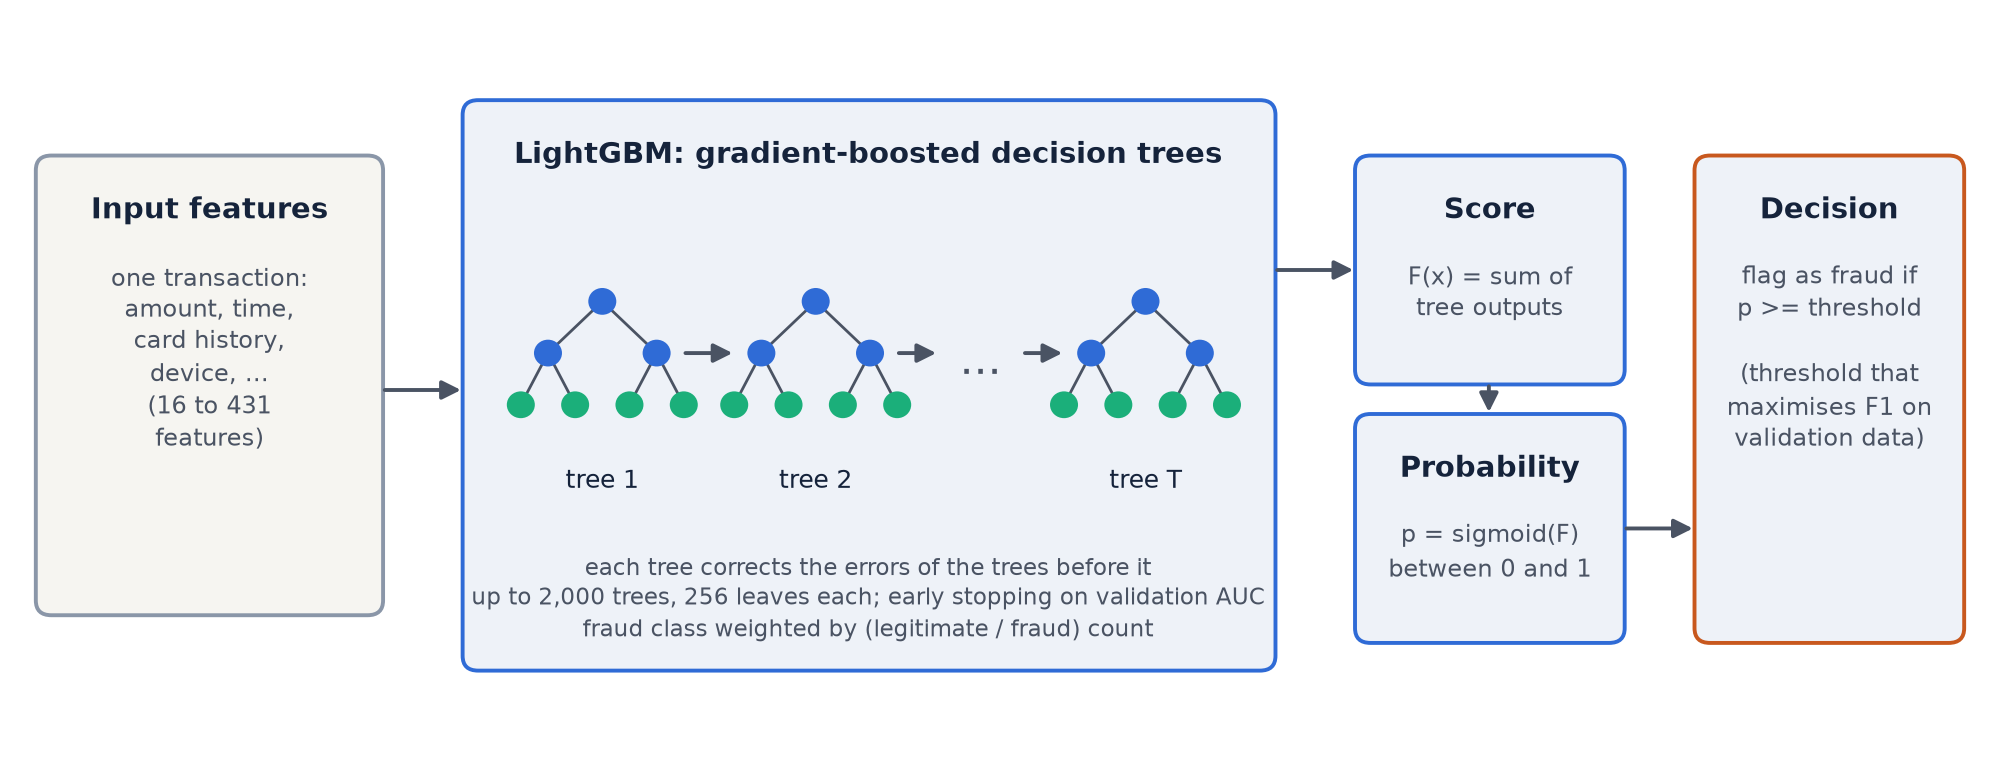
\includegraphics[width=0.95\textwidth]{figures/model_architecture.png}
  \caption*{Figure 4.3: Architecture of the fraud detection model: a transaction's features pass through a sequence of boosted decision trees, whose summed output becomes a fraud probability and, with the validation threshold, a decision}
\end{figure}

\begin{center}\small Table 4.4: LightGBM settings used for every model in the study\end{center}
\vspace{-1.2em}

{\small
\begin{longtable}{|>{\raggedright\arraybackslash}p{0.293\textwidth}|>{\raggedright\arraybackslash}p{0.293\textwidth}|>{\raggedright\arraybackslash}p{0.293\textwidth}|}
\hline
Setting & Value & Purpose \\ \hline
Objective & binary & Fraud probability for each transaction \\ \hline
Learning Rate & 0.05 & Step size of each boosting round \\ \hline
NUmber of leaves & 256 & Capacity of each tree \\ \hline
Minimum samples per leaf & 100 & Prevents leaves fitted to a few transactions \\ \hline
Row subsampling & 0.8,every round & Randomness and regularisation \\ \hline
Feature subsampling & 0.5 per tree & Randomness and regularisation \\ \hline
L2 regularisation & 1.0 & Shrinks leaf values \\ \hline
Class weight of fraud & legitimate / fraud count in the training data & Compensates for class imbalance \\ \hline
Boosting rounds & up to 2,000, early stopping after 100 without improvement & Stops on the validation part of the training window \\ \hline
Validation part & most recent 15\% of the training window & Early stopping, threshold choice and reference PR-AUC \\ \hline
\end{longtable}
}

The architecture of the fraud detection model: Features of a transaction are supplied to a chain of boosted decision tree models, whose total is a fraud probability that is utilised together with a validation threshold to make a judgement.  All training runs use a time-ordered validation split, where the most recent 15\% of the training window is held out for early stopping, selecting the decision threshold and tracking the model's reference PR-AUC. The decision threshold is the one that gives the best F1-score on this validation part. It is utilised for the F1-score, precision and recall reported accompanying PR-AUC and for the fraud flags returned by the scoring service. PR-AUC itself is not dependent on a threshold. Alessi and Fugini dynamically control the threshold 11 during the operation to balance precision and recall [16]. In this approach each model preserves the threshold selected in the training time, and a new threshold is associated to each re-trained model.

For the static baseline in RQ1 we use the first 50\% of each dataset for training, the following 10\% for validation and the following 40\% is split into ten consecutive time bins, so that we can track performance over the months after deployment.

\subsection*{4.2.2\quad Framework Architecture}
\addcontentsline{toc}{subsection}{4.2.2\quad Framework Architecture}

The framework translates the experimental results into a working MLOps system. Its components are depicted in figure 4.5 and its settings in table 4.5. It executes the loop from Figure 4.4 every seven days: monitor, decide, retrain, check, serve. Its decisions are tailored to weeks of label delay, not near-immediate feedback, so retraining is on a schedule, not driven by drift events; it integrates monitoring, retraining and deployment in one automated loop, like the closed-loop MLOps framework of Reda et al. for phishing detection [17].

\begin{figure}[H]
  \centering
  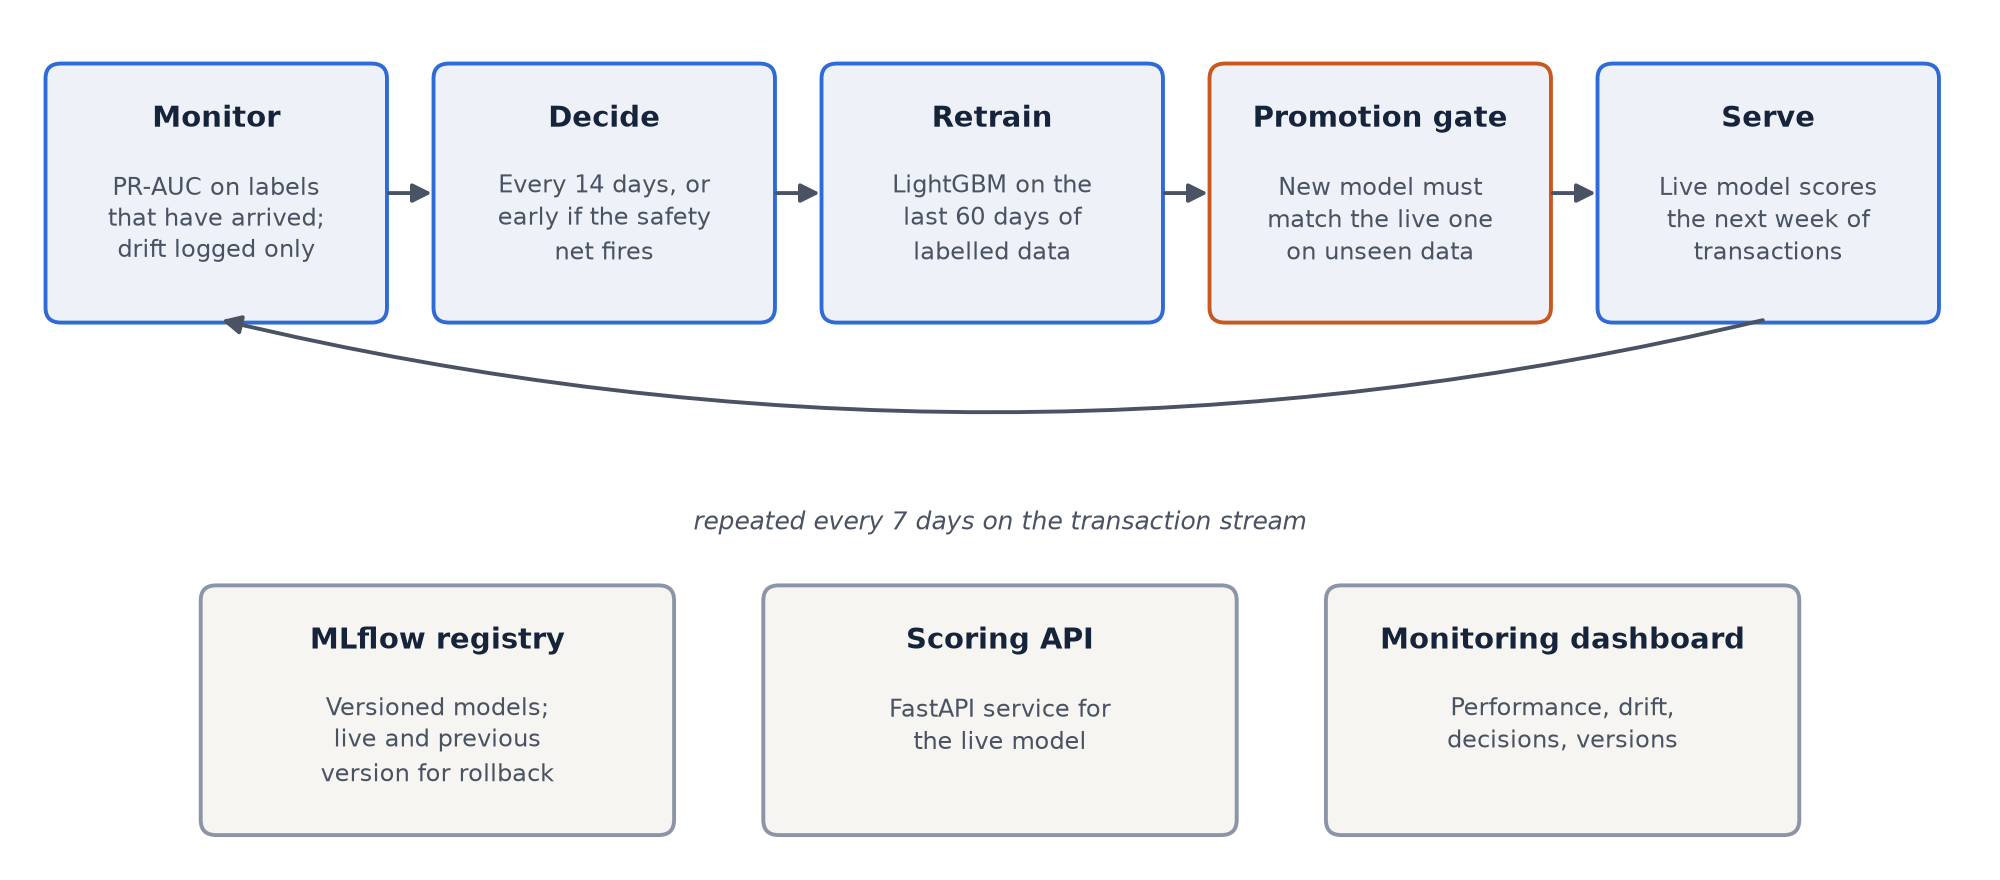
\includegraphics[width=0.95\textwidth]{figures/framework_loop.png}
  \caption*{Figure 4.4: The proposed continuous-learning loop, run every week on the transaction stream}
\end{figure}

\begin{figure}[H]
  \centering
  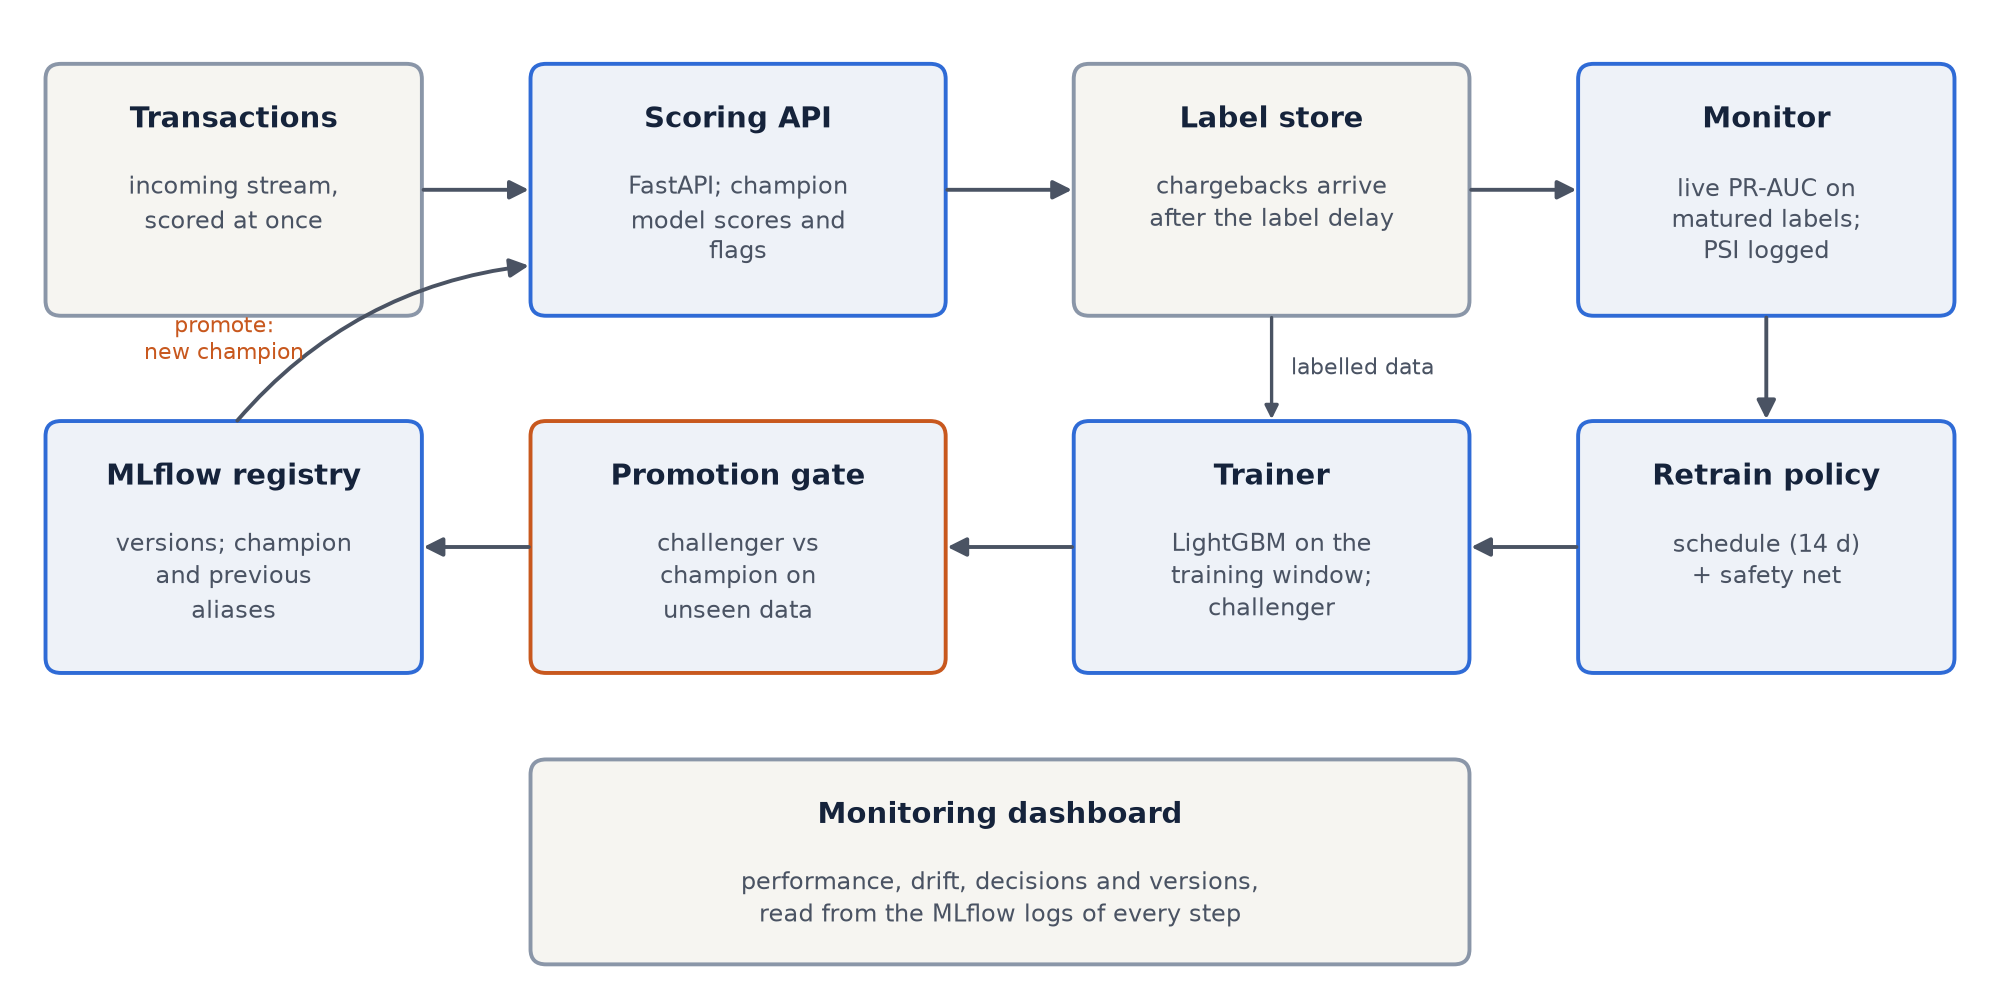
\includegraphics[width=0.95\textwidth]{figures/architecture.png}
  \caption*{Figure 4.5: Components of the proposed framework and the flow of data between them}
\end{figure}

\subsection*{4.2.3\quad Monitoring on Delayed Labels}
\addcontentsline{toc}{subsection}{4.2.3\quad Monitoring on Delayed Labels}

\textbf{The monitor calculates the PR-AUC of the live model on the labels that have matured} within the last 14 days, but only on transactions that the model was not trained on. It also determines the PSI of the model's scores and of its 10 most relevant numeric features against a sample of 50,000 rows of its training window and logs both to MLflow. The PSI is just logged for diagnosis purposes and never initiates retraining by itself, as expected by the trial results. Two types of monitoring are intentionally excluded from the current design: separate monitoring of the drift for each source of data, as is done in DriftGuard-TriAudit for numbers, text and layout of financial statements [18], and monitoring the stability of the model explanations, which John demonstrated can become unstable and unfair as populations drift [19]. Both are natural extensions when the framework is utilised with many data sources or when explanations are presented to investigators.

\subsection*{4.2.4\quad Retraining Policy and Safety Net}
\addcontentsline{toc}{subsection}{4.2.4\quad Retraining Policy and Safety Net}

The basic policy is a set schedule ; retrain a new model every 14 days on the latest 60 days of labelled data . The schedule is augmented with a safety net that retrains early, at most once every 7 days, when performance collapses between scheduled retrains:
\begin{equation*}
  \mathrm{AP}_{\mathrm{live}} < (1 - \tau)\,\max\big(\mathrm{AP}_{\mathrm{val}},\ \mathrm{median}_{4}(\mathrm{AP}_{\mathrm{live}})\big) \quad\text{or}\quad \mathrm{AP}_{\mathrm{live}} < \lambda\,\pi \tag{4.7}
\end{equation*}
with $\tau = 0.30$, $\lambda = 3$ and $\pi$ the fraud rate among the matured labels. The first condition compares the live PR-AUC to the best of the model's own validation PR-AUC and the median of the last four live measurements. Recent live history is also important, as is using the validation score. A model trained on corrupted data can claim a poor validation score, which would otherwise lower the bar it is assessed against. The other condition is a no-skill check, as a skill-less model gives a PR-AUC close to the fraud rate.

\subsection*{4.2.5\quad Training and Automatic Window Selection}
\addcontentsline{toc}{subsection}{4.2.5\quad Training and Automatic Window Selection}

The trainer trains a LightGBM model with the parameters of Table 4.4, on the policy's training window, which is one label delay before the present. A window length of zero is possible for an expanding window. Each new model is registered in MLflow as a challenger along with its training window, validation PR-AUC and threshold.

\textbf{Automatic window picking}: The trials indicated that the ideal training window depended on the dataset, 60 days on IEEE-CIS but full labelled history on Sparkov and BAF. A fixed window chosen on one dataset may be incorrect for another. So the framework can select the window itself. At each retrain it trains one challenger $m_w$ per candidate window $w$, here the last 60 days and all labelled history, and scores all of them on the same evaluation rows $E$: the most recent labelled transactions that none of the candidates was trained on and the champion was not trained on either. It only keeps
\begin{equation*}
  w^{*} = \arg\max_{w \in \mathcal{W}} \mathrm{AP}_{E}(m_w), \qquad \mathcal{W} = \{\text{60 days},\ \text{all history}\} \tag{4.8}
\end{equation*}
and only this challenger proceeds to the promotion gate, the rest are noted as not picked. The option depends solely on data that would be accessible at the time, and has no need for knowing which window is appropriate for the dataset. The extra cost is one extra training run per retrain as the candidates are trained on the same data except for their start date.

\subsection*{4.2.6\quad Promotion Gate}
\addcontentsline{toc}{subsection}{4.2.6\quad Promotion Gate}

In the champion-challenger pattern of MLOps practice [7], [20], a challenger replaces the live model (the champion) if it clears the promotion gate. The gate evaluates both models on the challenger's validation data, which is restricted to transactions not observed by the champion at training, thus neither model is evaluated on data it has observed. The challenger is promoted if
\begin{equation*}
  \mathrm{AP}(\text{challenger}) \ge \mathrm{AP}(\text{champion}) - \delta \tag{4.9}
\end{equation*}
where $\delta = 0.01$. Both models are re-scored via the production feature path, not with scores saved at training time. This is the key: a model trained on incorrectly scaled features appears excellent on its own, equally incorrect, validation data, but fails on the inputs it will actually receive in production. If the comparison data contains less than 30frauds the comparison is unreliable and the challenger is promoted by default.

\subsection*{4.2.7\quad Framework Configuration}
\addcontentsline{toc}{subsection}{4.2.7\quad Framework Configuration}

\begin{center}\small Table 4.5: Settings of the framework (configs/default.toml)\end{center}
\vspace{-1.2em}

{\small
\begin{longtable}{|>{\raggedright\arraybackslash}p{0.293\textwidth}|>{\raggedright\arraybackslash}p{0.293\textwidth}|>{\raggedright\arraybackslash}p{0.293\textwidth}|}
\hline
Setting & Value & Meaning \\ \hline
Loop interval & 7 days & How often the framework monitors, decides and serves \\ \hline
Label delay d & 30 days & Labels usable this long after the transaction \\ \hline
Retraining schedule & 14 days & Primary policy \\ \hline
Training window & 60 days & Sliding window of labelled data (0 = expanding) \\ \hline
Candidate windows & 60 days,all & With automatic selection: one challenger per window, the best one is gated \\ \hline
Monitoring window & 14 days & Matured labels used for live PR-AUC \\ \hline
Minimum frauds & 30 & Fewer frauds: live PR-AUC is not computed \\ \hline
Safety-net tolerance $\tau$ & 0.30 & Relative drop that triggers an early retrain \\ \hline
History for the reference & 4 & Recent live measurements in the median \\ \hline
No-skill factor $\lambda$ & 3 & Live PR-AUC below 3 x fraud rate triggers \\ \hline
Minimum gap between retrains & 7 days & Prevents repeated early retrains \\ \hline
Gate tolerance $\delta$ & 0.01 & Largest PR-AUC loss a challenger may show \\ \hline
Gate minimum frauds & 30 & Fewer frauds: the challenger is promoted by default \\ \hline
Drift features tracked & 10 & Most important numeric features (PSI logged) \\ \hline
\end{longtable}
}

\section*{4.3\quad Data Collection}
\addcontentsline{toc}{section}{4.3\quad Data Collection}

The study employs three available datasets on fraud, which are presented in Table 4.6. Reliable timestamps in public data are crucial to the study questions, because drift and label delay can only be studied when transactions can be replayed in the order they occurred. Therefore, commonly used fraud datasets that cover only a few days [14], [12] were not appropriate.

\begin{center}\small Table 4.6: Sources of the datasets\end{center}
\vspace{-1.2em}

{\small
\begin{longtable}{|>{\raggedright\arraybackslash}p{0.124\textwidth}|>{\raggedright\arraybackslash}p{0.316\textwidth}|>{\raggedright\arraybackslash}p{0.207\textwidth}|>{\raggedright\arraybackslash}p{0.233\textwidth}|}
\hline
Dataset & Source & Final used & Records in the source \\ \hline
IEEE-CIS & Kaggle competition IEEE-CIS Fraud Detection (IEEE Computational Intelligence Society and Vesta Corporation) & train transaction.csv, \_ train identity.csv \_ & 590,540 transactions \\ \hline
Sparkov & Kaggle dataset Credit Card Transactions Fraud Detection (generated with the Sparkov simulator) & fraudTrain.csv, fraudTest.csv & 1,852,394 transactions \\ \hline
BAF & Kaggle dataset Bank Account Fraud Dataset Suite (NeurIPS 2022) & Base.csv (of six variants) & 1,000,000transactions \\ \hline
\end{longtable}
}

The three datasets were all retrieved from Kaggle. IEEE-CIS is a competition dataset and participation needs acceptance of the competition regulations. Its test files were not used and are unlabelled. Sparkov is separated into two files covering one continuous era, both were merged. BAF was supplied as a basic dataset and five variations with controlled bias, and the base dataset was used. The code does not share the raw data: the scripts used to prepare it are in the repository to allow the regeneration of all results from the original sources. Two practical decisions made data collecting replicable. First, a preparation script transforms each dataset into the same table layout, so all tests are executed without change on any of them. Second, the long experiments on the two bigger replication datasets were run as Kaggle notebooks, next to the data, with the code downloaded directly from the public repo.

\section*{4.4\quad Dataset Overview}
\addcontentsline{toc}{section}{4.4\quad Dataset Overview}

This section describes each dataset, the target variable, the cleaning and feature engineering applied to it, and the resulting preprocessed data.

\subsection*{4.4.1\quad IEEE-CIS Fraud Detection}
\addcontentsline{toc}{subsection}{4.4.1\quad IEEE-CIS Fraud Detection}

The major dataset is IEEE-CIS. It was published by IEEE Computational Intelligence Society and Vesta Corporation. It has 590540 genuine e-commerce transactions over 182 days and 3.5\% of them are fake. It has been employed in recent works on drift and fraud detection [4], [10]. The transaction and identity data are merged on the transaction identifier, yielding 431 features, most of which are anonymised by the provider. Only the time column (seconds from a reference point), identifier, and label are omitted. LightGBM handles text columns as categorical features natively, and missing values are left as missing rather than filled in. More than 50\% of the transactions are missing for more than 50\% of the columns.

\subsection*{4.4.2\quad Sparkov Credit Card Transactions}
\addcontentsline{toc}{subsection}{4.4.2\quad Sparkov Credit Card Transactions}

The first dataset to replicate is Sparkov . It includes around 1,000 customers' card transactions, generated using the Sparkov transaction simulator from January 2019 to December 2020. We cut the data at 21 December 2020 after inspection, because the simulator creates nearly no fraud after that date (17 frauds and then none, although the volume doubles), which would render the following weeks irrelevant for evaluation. For the other 1,801,969 transactions we have 720 days and a fraud rate of 0.53\%. We have deleted names, street addresses, card numbers and transaction numbers. We extract the transaction hour and weekday, the customer's age and the distance between customer and merchant, and five per-card behaviour features: the time since the last transaction with the card, its number and total amount of transactions in the previous 24 hours, its number of transactions in the previous 30 days and the amount relative to the card's running average. Each of them is calculated purely based on past transactions from the card, therefore a feature never contains information from the future. We purposefully did not utilise a lifetime transaction count, because it only rises with time and would drift by construction.

\subsection*{4.4.3\quad Bank Account Fraud (BAF)}
\addcontentsline{toc}{subsection}{4.4.3\quad Bank Account Fraud (BAF)}

The second replication data set is BAF. Privacy-preserving synthetic dataset of 1 million bank account applications over 8 months. Generated from real data, it is supposed to have realistic drift across months. The one we use is Base. Missing values (negative values in six columns) as documented by the providers are transformed to missing values. A constant column is eliminated and the month itself is not used as a feature, so that the model can not memorise the period. Because BAF only captures the month of each application, we use a predetermined seed to assign each record a random time within the month. Thus drift manifests itself between months, but the weeks inside a month are interchangeable. This is a limitation of the dataset, and the BAF results are interpreted as such.

\subsection*{4.4.4\quad Target Variable and Class Imbalance}
\addcontentsline{toc}{subsection}{4.4.4\quad Target Variable and Class Imbalance}

The target is a binary label classifying a transaction, or an application in the case of BAF, as fraudulent (1) or legal (0). It is termed isFraud by IEEE-CIS, is\_fraud by Sparkov and fraud\_bool by BAF. All three rename it isFraud. Fraud is rare in each dataset, the ratio of valid transactions to fraud is 27.6 for IEEE-CIS, 186.1 for Sparkov and 89.7 for BAF. Hence, accuracy is not a metric (a model that never predicts fraud would be 96.5\% to 99.5\% accurate) and PR-AUC is the primary metric (Section 4.1.4). We weight the fraud class in training to account for the imbalance. We do not utilise any oversampling such as SMOTE as resampling can overstate the performance [14].

\subsection*{4.4.5\quad Data Cleaning and Feature Engineering}
\addcontentsline{toc}{subsection}{4.4.5\quad Data Cleaning and Feature Engineering}

The preprocessing workflow is depicted in Figure 4.6. In IEEE-CIS, the transaction and identity tables are connected on transaction identifier, numeric columns are stored in the smallest suitable form to save memory, and the 31 text columns are converted to category characteristics. Missing values are kept missing, since LightGBM handles them natively and because missingness in itself might be informative: 214 of the 434 columns are missing for more than half of the transactions. In Sparkov, names, street addresses, card numbers and transaction numbers are redacted. The data is truncated at 21 December 2020, after which the simulator creates almost no fraud. This results in 1,801,969 out of 1,852,394 transactions being kept. Time-of-day, weekday, age and the distance between client and merchant are calculated, and five per-card behaviour traits are computed solely from each card's previous transactions, so that no information leaks from the future. In BAF, missing values (negative values in six columns) are transformed to missing, a constant column is eliminated, and the month is not used as a feature.

\begin{figure}[H]
  \centering
  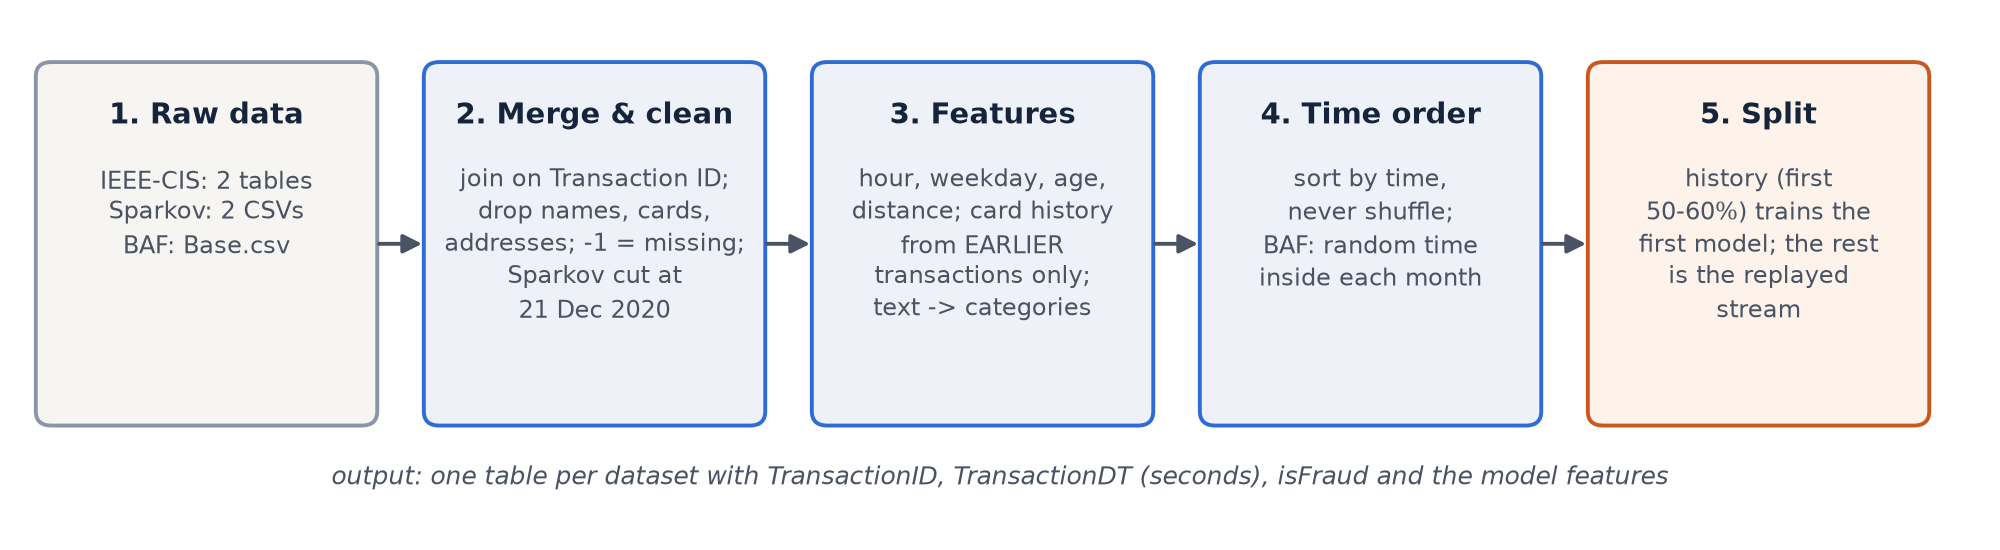
\includegraphics[width=0.95\textwidth]{figures/preprocessing.png}
  \caption*{Figure 4.6: Preprocessing pipeline from the raw files of each dataset to the common time-ordered table}
\end{figure}

\subsection*{4.4.6\quad Time Ordering and History-Stream Split}
\addcontentsline{toc}{subsection}{4.4.6\quad Time Ordering and History-Stream Split}

All three datasets are sorted by time and never jumbled . Each is divided into a history, used to train the first model, and a stream, which is repeated as if it was arriving live, at a defined fraction of its rows (Figure 4.7). The stream begins at 60\% of the rows for IEEE-CIS (day 101), and at 50\% for Sparkov and BAF, whose lengthier histories offer a full year or four months of training data prior to deployment

\begin{figure}[H]
  \centering
  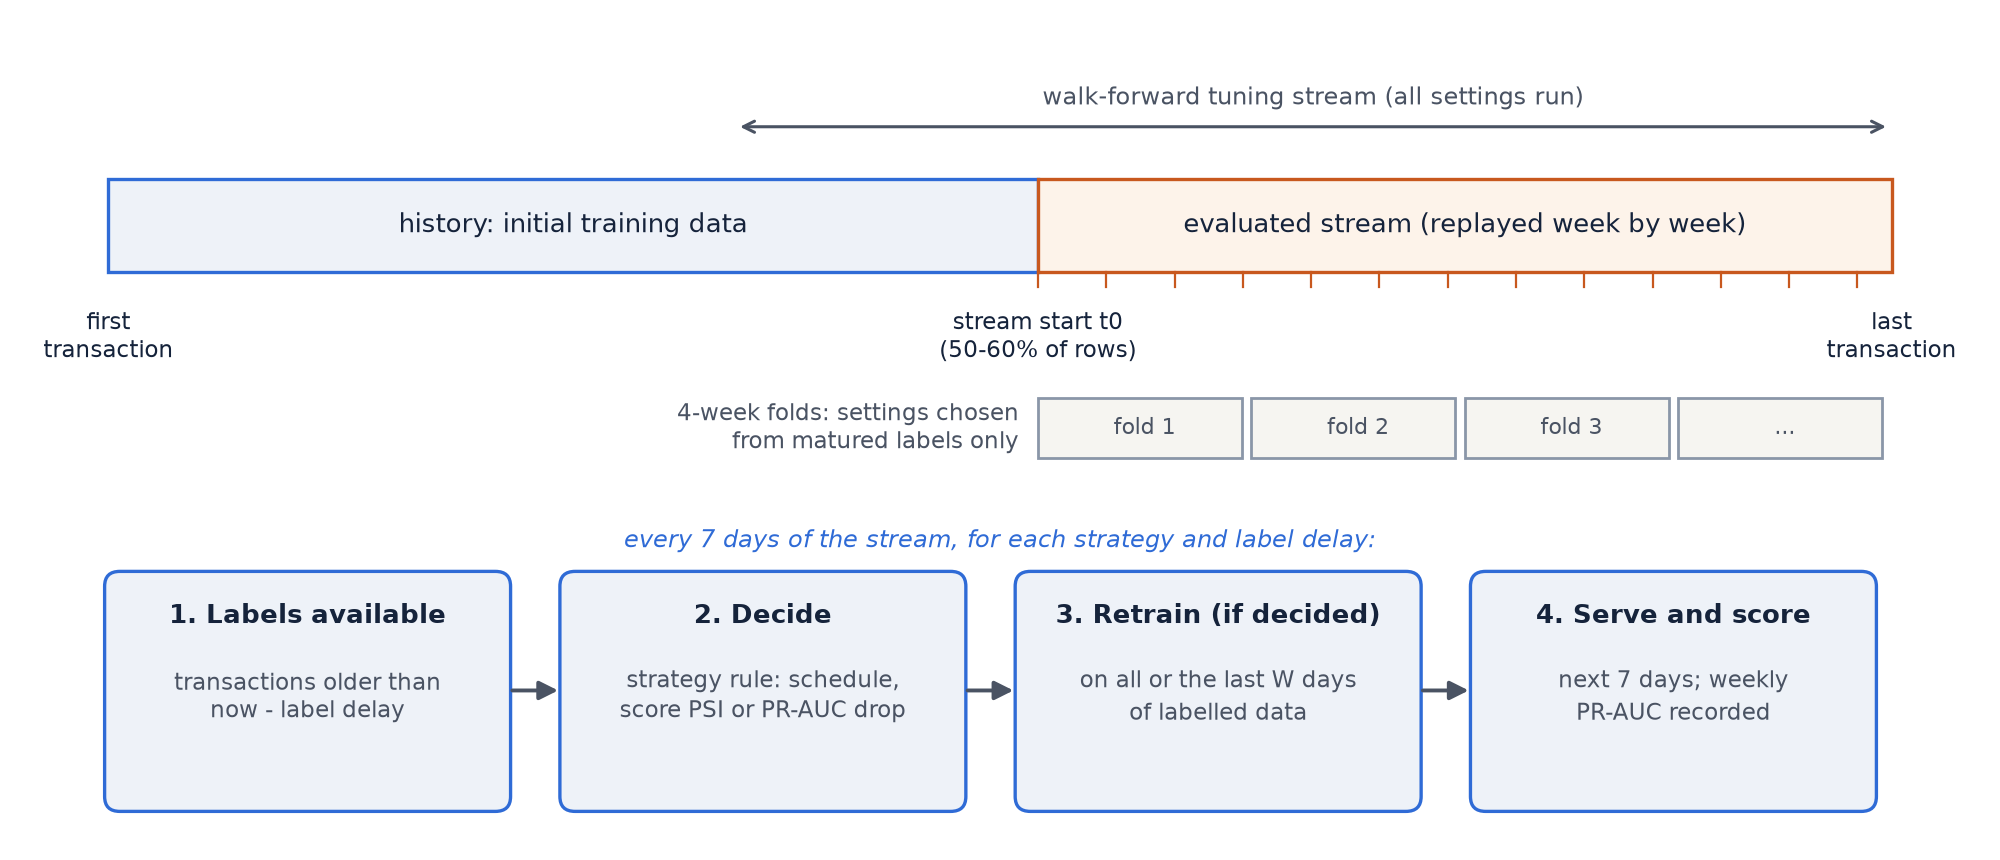
\includegraphics[width=0.95\textwidth]{figures/protocol.png}
  \caption*{Figure 4.7: Evaluation protocol: each dataset is split in time into a history and a stream that is replayed week by week; settings are tuned walk-forward in 4-week folds}
\end{figure}

\subsection*{4.4.7\quad Summary of Preprocessed Data}
\addcontentsline{toc}{subsection}{4.4.7\quad Summary of Preprocessed Data}

Table 4.7 summarises the data after preprocessing, and Table 4.8 compares the three datasets. Every prepared dataset is a single table with a transaction identifier, a time column in seconds, the isFraud label and the model features, sorted by time

\begin{center}\small Table 4.7: Summary of the preprocessed data\end{center}
\vspace{-1.2em}

{\small
\begin{longtable}{|>{\raggedright\arraybackslash}p{0.222\textwidth}|>{\raggedright\arraybackslash}p{0.218\textwidth}|>{\raggedright\arraybackslash}p{0.222\textwidth}|>{\raggedright\arraybackslash}p{0.218\textwidth}|}
\hline
 & IEEE-CIS & Sparkov & BAF \\ \hline
Records after preprocessing & 590,540 & 1,801,969 & 1,000,000 \\ \hline
Frauds(rate) & 20,663 (3.50\%) & 9,634 (0.53\%) & 11,029 (1.10\%) \\ \hline
Legitimate per fraud & 27.6 & 186.1 & 89.7 \\ \hline
Features (of which categorical) & 421 (31) & 16 (5) & 29 (5) \\ \hline
History: training the first model & 354,324 (60\%) & 900,984 (50\%) & 500,000 (50\%) \\ \hline
Stream: played week by & 236,216(12 weeks) & 900,985 (52 weeks) & 500,000 (19 weeks) \\ \hline
week &  &  &  \\ \hline
\end{longtable}
}

\begin{center}\small Table 4.8: Datasets used in this study (after preparation)\end{center}
\vspace{-1.2em}

{\small
\begin{longtable}{|>{\raggedright\arraybackslash}p{0.165\textwidth}|>{\raggedright\arraybackslash}p{0.275\textwidth}|>{\raggedright\arraybackslash}p{0.222\textwidth}|>{\raggedright\arraybackslash}p{0.218\textwidth}|}
\hline
 & IEEE-CIS & Sparkov & BAF(Base) \\ \hline
Domain & Real e-commerce card transaction (Vesta) & Simulated card transactions (Sparkov generator) & Bank account opening applications (privacy-preserving synthetic data) \\ \hline
Records & 590,540 & 1,801,969 & 1,000,000 \\ \hline
Time span & 182 days & 720 days ( to 21 Dec 2020) & 8 months \\ \hline
Fraud rate & 3.50\% & 0.53\% & 1.10\% \\ \hline
Features used & 431 (transaction and identity tables, mostly anonymised) & 16 (amount, time, location, customer and card-history features) & 29 (applicant, request, device and velocity features) \\ \hline
Time resolution & Seconds from a reference point & Exact timestamp & Month only (time within the month assigned at random) \\ \hline
Stream starts at & 60\% of rows (day 101) & 50\% of rows (about 1 Jan 2020) & 50\% of rows (month 4) \\ \hline
Role & Main dataset & Replication & Second replication \\ \hline
\end{longtable}
}

\section*{4.5\quad Project Management Plan}
\addcontentsline{toc}{section}{4.5\quad Project Management Plan}

The project was arranged in three stages according to the thesis deliverables as illustrated in Figure 4.8. The first phase was the literature review, the research questions and the production of IEEE-CIS. The second stage comprised the experiments, their statistical validation and the framework design. The third stage included the evaluation of the framework, the replication on two more datasets, automatic window selection and the desired improvements in the supervisor feedback .

\begin{figure}[H]
  \centering
  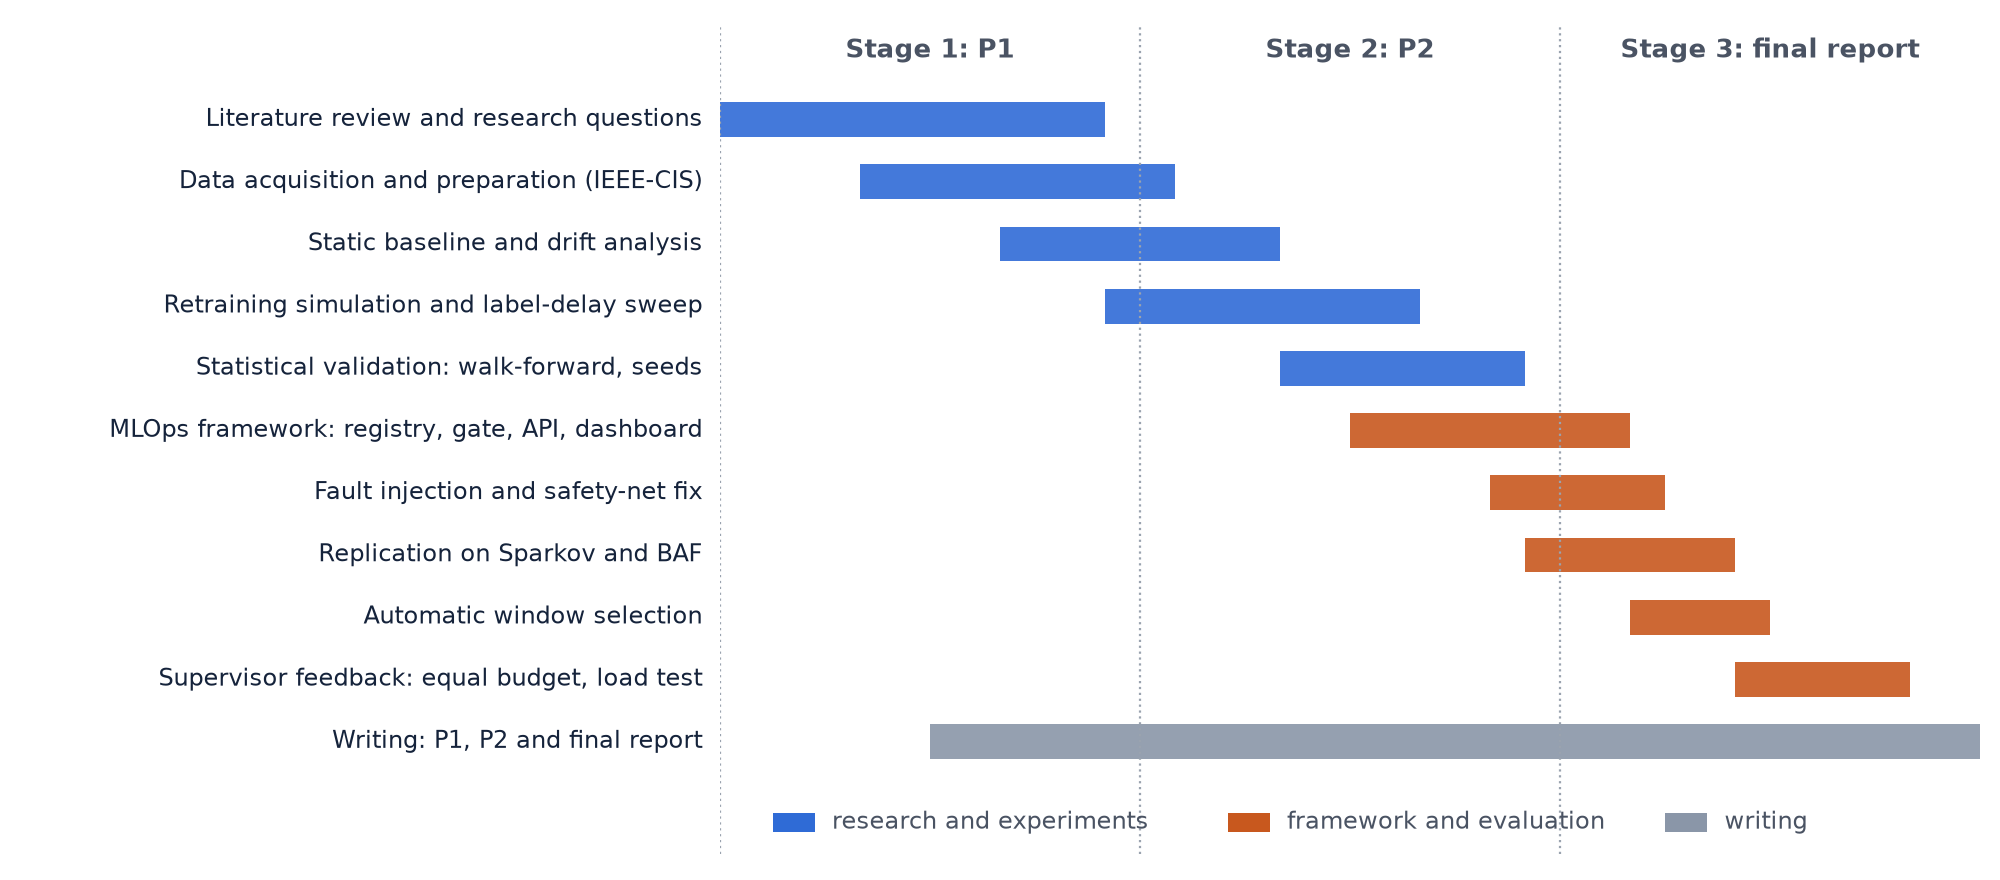
\includegraphics[width=0.95\textwidth]{figures/project_plan.png}
  \caption*{Figure 4.8: Project management plan over the three thesis stages}
\end{figure}

Experiments were performed in brief iterations: plan, do, review and if the result suggested a new question, another experiment was performed. This cycle led to a couple of design decisions. The walk-forward tuning was added when fixed tuning periods were too short to rank the drift triggers, the promotion gate was changed to re-score models on production features after a fault test exposed a weakness and automatic window selection was added when the replication showed that the best window depends on the dataset. Supervisor comments was also incorporated in this manner, for example the equal-budget comparison in Section 5.2.2. All code and configuration was stored in a Git repository on GitHub and every update was followed by an automated test suite. Because the experiments are extensive (many hours) and there are power cuts, the results are saved after each step and the experiments are continued from there. The longest runs were moved to Kaggle notebooks.

\section*{4.6\quad Implementation of Selected Design}
\addcontentsline{toc}{section}{4.6\quad Implementation of Selected Design}

The selected design was implemented as a Python package with a back end that runs the continuous learning loop, a front end for monitoring, and a model registry that connects them. Table 4.9 lists the modules.

\subsection*{4.6.1\quad Back End}
\addcontentsline{toc}{subsection}{4.6.1\quad Back End}

\begin{center}\small Table 4.9: Modules of the framework (Python package fraud\_mlops)\end{center}
\vspace{-1.2em}

{\small
\begin{longtable}{|>{\raggedright\arraybackslash}p{0.237\textwidth}|>{\raggedright\arraybackslash}p{0.643\textwidth}|}
\hline
Module & Responsibility \\ \hline
config & Typed configuration loaded from one TOML file per dataset \\ \hline
data & Loading, caching and time-window access to the transaction table \\ \hline
training & LightGBM training on a window with a time-ordered validation split \\ \hline
model & Scoring of raw input, including missing columns and text categories \\ \hline
monitoring & Live PR-AUC on matured labels; PSI of scores and features \\ \hline
policy & Retraining policy, safety net, candidate windows and promotion gate \\ \hline
registry & MLflow runs and model registry with champion and previous aliases \\ \hline
pipeline & The replay loop: monitor, decide, retrain, gate and serve \\ \hline
faults & Fault injection for testing the safeguards \\ \hline
serving & FastAPI scoring service for the champion model \\ \hline
dashboard & Self-contained HTML monitoring dashboard \\ \hline
cli & Command line: replay, champion, dashboard and serve \\ \hline
\end{longtable}
}

The study is implemented in Python with LightGBM, pandas, NumPy and scikit-learn for the experiments, MLflow with a SQLite backend for tracking and the model registry, and FastAPI for the scoring service. The framework is a Python package which consists of 21 distinct modules for setup, data access, training, monitoring, retraining policy, promotion gate, registry, fault injection, serving and the dashboard, and is configured with one TOML file per dataset. The components and the whole loop are tested on modest synthetic data using 24 automated tests. Command line driven for the back end. replay performs the loop over a dataset as if it was live, champion reports the model in service, dashboard produces the monitoring dashboard and serve starts the scoring service. Each training run is stored in MLflow with its parameters, metrics and training window. Each model is registered as a new version.

\subsection*{4.6.2\quad Front End}
\addcontentsline{toc}{subsection}{4.6.2\quad Front End}

The front end is a monitoring dashboard generated as a single HTML page from the MLflow logs of a replay. This can be opened in any browser without a server. It shows the summary numbers of the run, the weekly performance of the served model together with what the loop could measure on delayed labels and the safety-net line (Figure 4.9), the drift measures, every retraining decision with its reason, and the history of model versions with the champion and the version kept for rollback (Figure 4.10).

\begin{figure}[H]
  \centering
  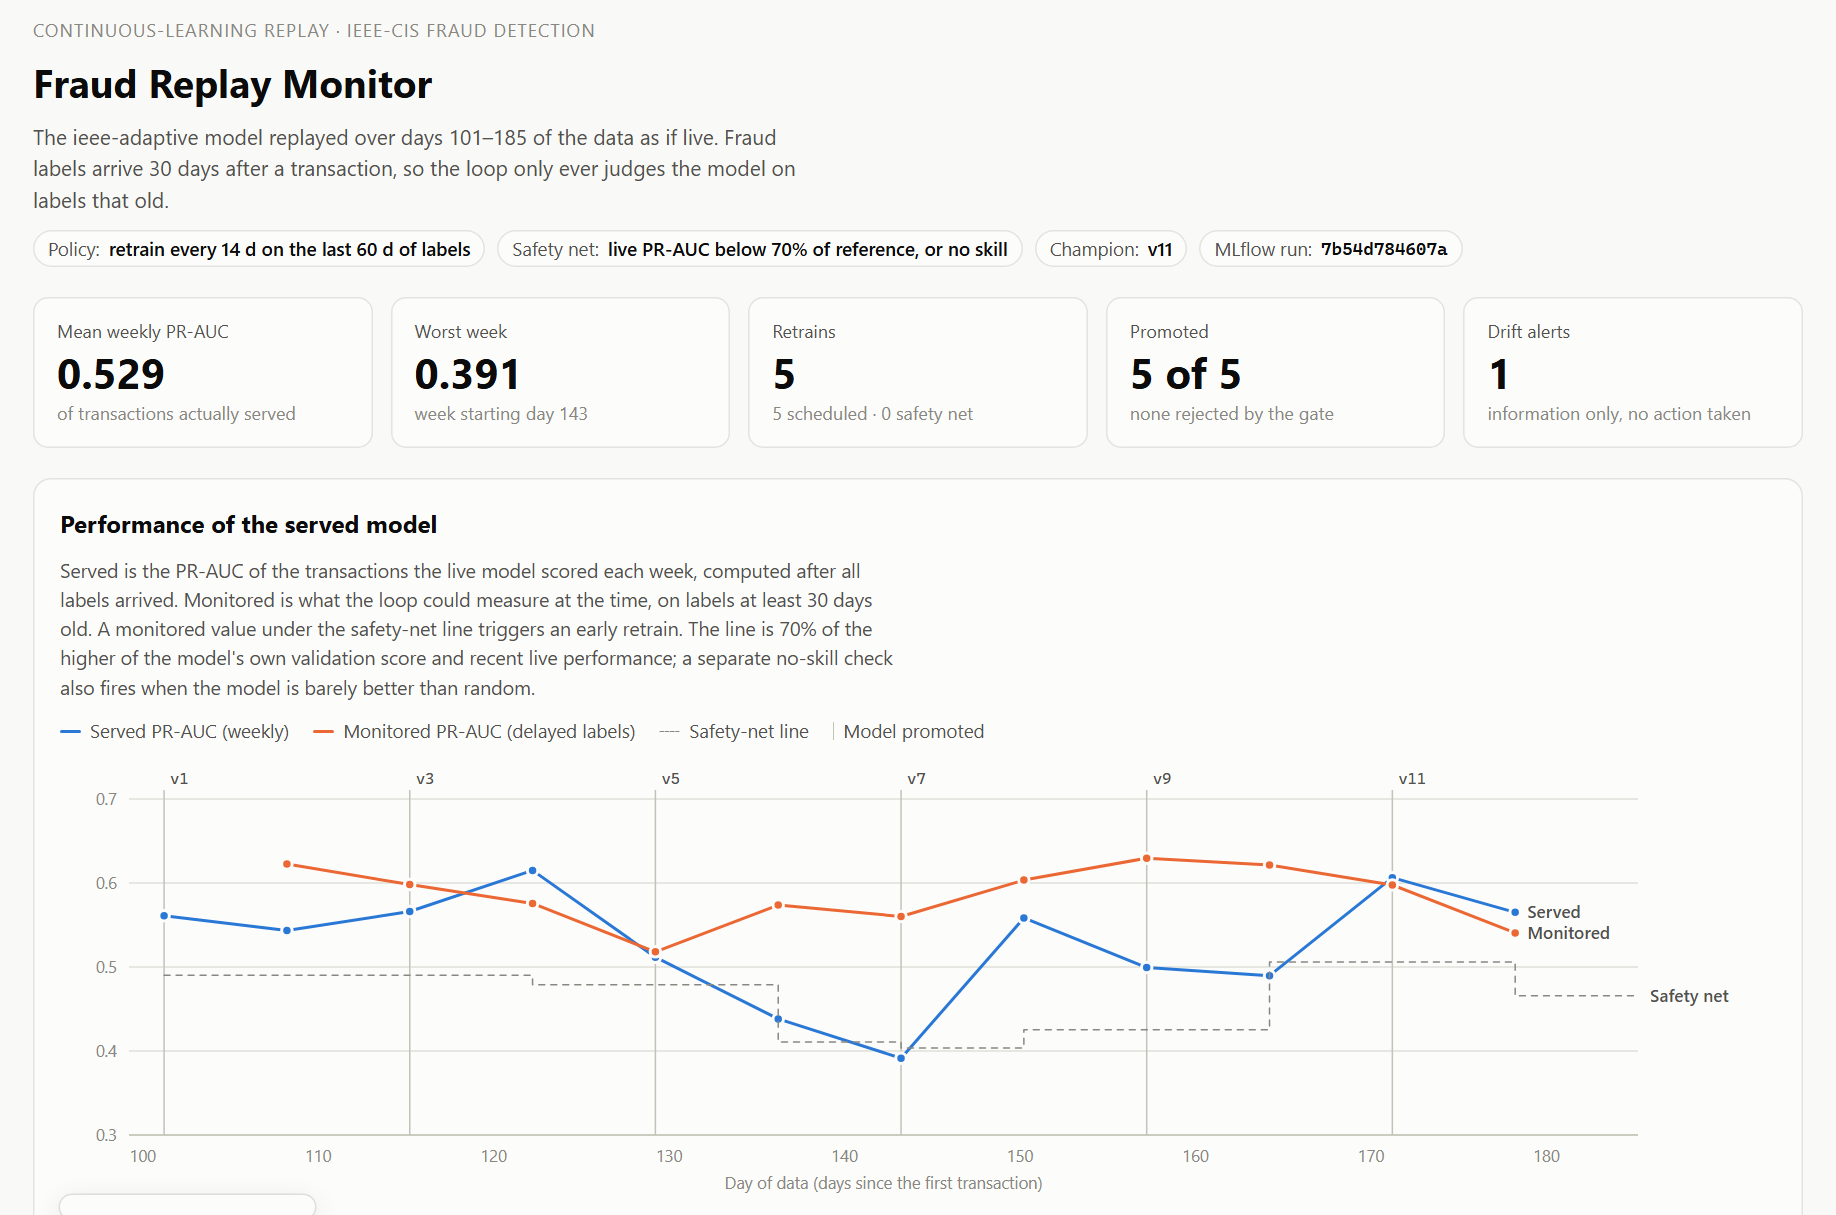
\includegraphics[width=0.95\textwidth]{figures/dashboard_top.png}
  \caption*{Figure 4.9: Front end: the monitoring dashboard after a replay of IEEE-CIS (summary figures and the performance of the served model)}
\end{figure}

\begin{figure}[H]
  \centering
  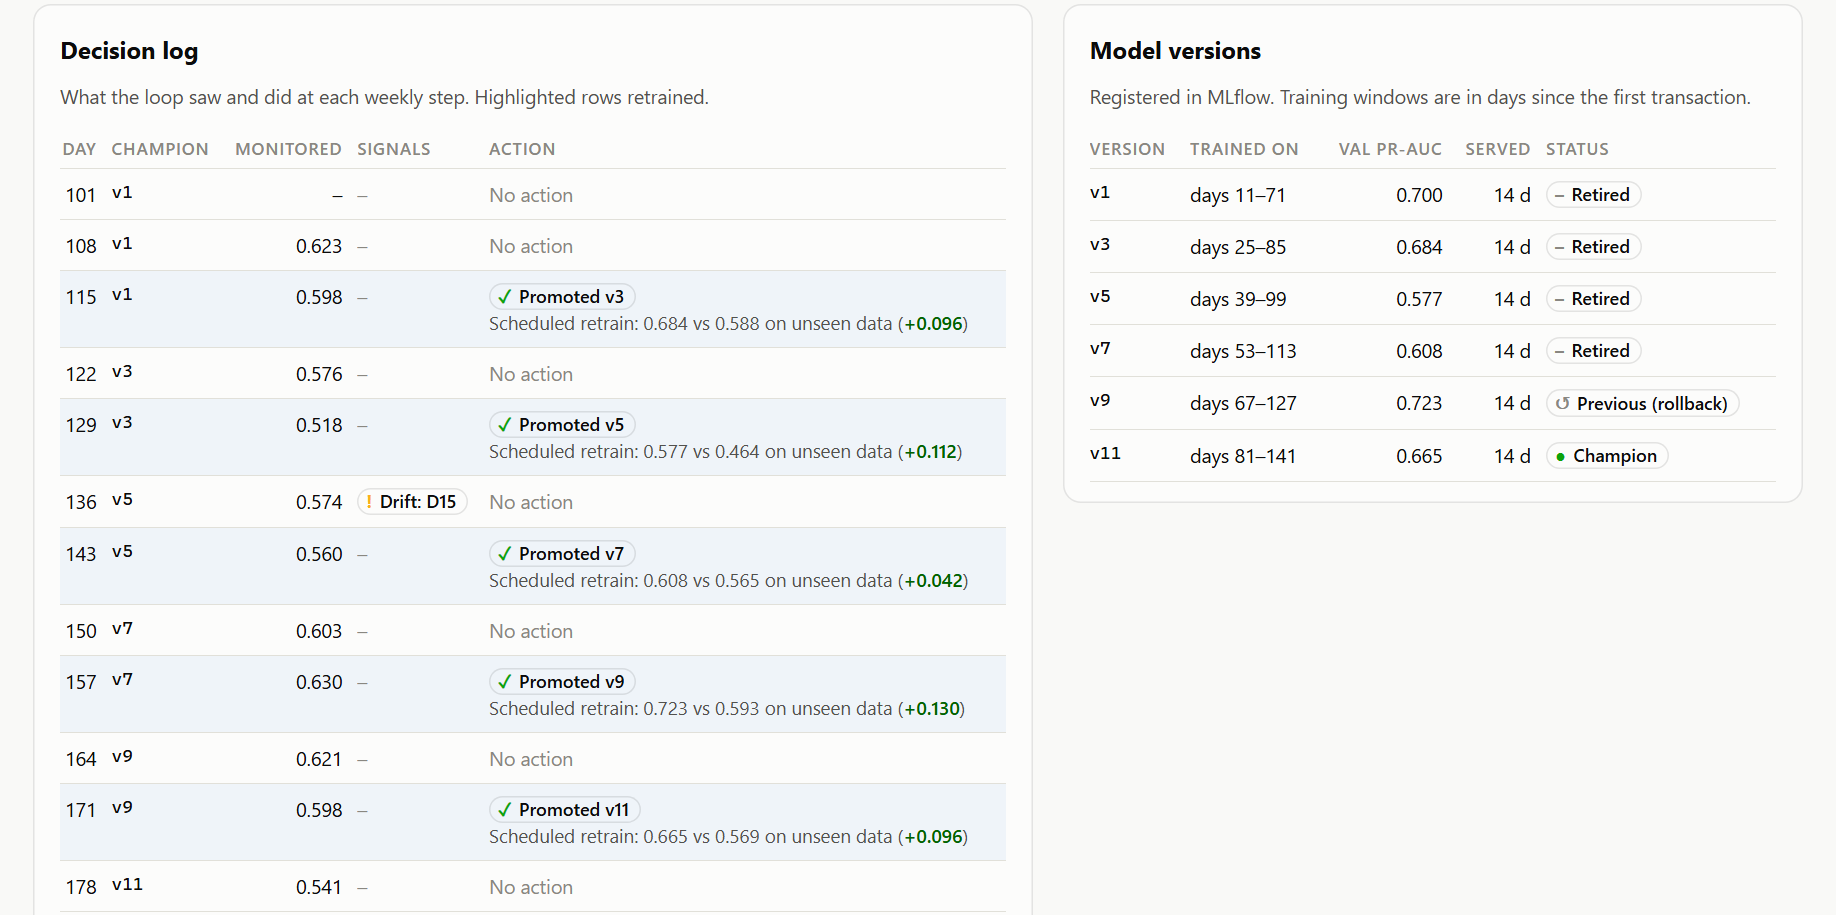
\includegraphics[width=0.95\textwidth]{figures/dashboard_log.png}
  \caption*{Figure 4.10: Front end: decision log and model versions on the monitoring dashboard}
\end{figure}

\subsection*{4.6.3\quad Frontend-Backend Integration}
\addcontentsline{toc}{subsection}{4.6.3\quad Frontend-Backend Integration}

Each model version is saved with its parameters, metrics and training window using MLflow. The in service model has the alias champion and its predecessor the alias previous thus a rollback is a single alias change. A FastAPI service loads the champion and has three endpoints: /health returns the version being served up, /predict returns a fraud chance and flag for each input transaction, and /reload switches to a newly promoted champion without a restart. The monitoring dashboard created from the MLflow logs shows weekly performance, drift, every retraining choice with its justification, and the history of model versions. The MLflow model registry is the contract between the parts: the back end writes model versions and moves the champion alias when the promotion gate accepts a challenger, the scoring service loads whatever carries that alias and reloads it on request, and the dashboard reads the same registry and run logs. no component needs to know what the other components are doing, hence the scoring service always returns the model that the gate last authorised

\setcounter{chapter}{4}
\chapter{Result Analysis}

\section*{5.1\quad Performance Evaluation}
\addcontentsline{toc}{section}{5.1\quad Performance Evaluation}

\subsection*{5.1.1\quad Testing Method}
\addcontentsline{toc}{subsection}{5.1.1\quad Testing Method}

We evaluate the framework and the retraining strategies by replaying each dataset in strict time order as outlined in Section 4.1. We train a model on the history, deploy it at the start of the stream and score each following week before the labels of that week are available, the labels become only usable after the label delay of 0, 15, 30 or 60 days. All strategies begin with the same baseline model and view identical data, meaning that the only thing that differentiates the strategies is their retraining decisions. The framework itself is tested via a full replay with its register, monitor and promotion gate (Section 5.2.3) and by injecting defects into its retraining jobs (Section 5.2.4).

\subsection*{5.1.2\quad Evaluation Metrics}
\addcontentsline{toc}{subsection}{5.1.2\quad Evaluation Metrics}

The basic statistic is the mean weekly PR-AUC (Equation 4.5) calculated per week such that scores of different model versions are never merged. Secondary measures include ROC-AUC, precision, recall and F1 at each model's validation threshold, lowest weekly PR-AUC, and number of retrains. Drift is computed using the PSI (Eq. 4.3). Differences between methods are provided using 95\% paired day-block bootstrap intervals, and a difference is considered reliable when its interval excludes zero. The datasets differ in difficulty so a model without skill would score 0.035 on IEEE-CIS, 0.005 on Sparkov and 0.011 on BAF. So, PR-AUC values are compared only within a dataset.

\subsection*{5.1.3\quad Model Performance and Drift after Deployment}
\addcontentsline{toc}{subsection}{5.1.3\quad Model Performance and Drift after Deployment}

Table 5.1 and Figure 5.1 show how the static model performed over the test period of each dataset, which follows the training and validation periods in time.

\begin{center}\small Table 5.1: Performance of the static model and drift of its inputs after deployment\end{center}
\vspace{-1.2em}

{\small
\begin{longtable}{|>{\raggedright\arraybackslash}p{0.222\textwidth}|>{\raggedright\arraybackslash}p{0.218\textwidth}|>{\raggedright\arraybackslash}p{0.222\textwidth}|>{\raggedright\arraybackslash}p{0.218\textwidth}|}
\hline
 & IEEE-CIS & Sparkov & BAF \\ \hline
PR-AUC over the whole test period & 0.510 & 0.936 & 0.164 \\ \hline
ROC-AUC over the whole test period & 0.888 & 0.997 & 0.871 \\ \hline
PR-AUC, first time bin & 0.581 & 0.954 & 0.164 \\ \hline
PR-AUC, lowest time bin & 0.388 (bin 6) & 0.893(bin 10) & 0.169(bin 6) \\ \hline
PR-AUC, last time bin & 0.534 & 0.893 & 0.169 \\ \hline
Largest feature PSI (feature) & 0.17 (D10) & 0.53 (card txns 24h) \_ \_ & 4.60 (velocity 4w) \_ \\ \hline
Score-PSI trigger (threshold 0.1) & Never fired; maximum score PSI 0.017 & Fired once (1 of 4 label delays) & Never fired \\ \hline
\end{longtable}
}

\begin{figure}[H]
  \centering
  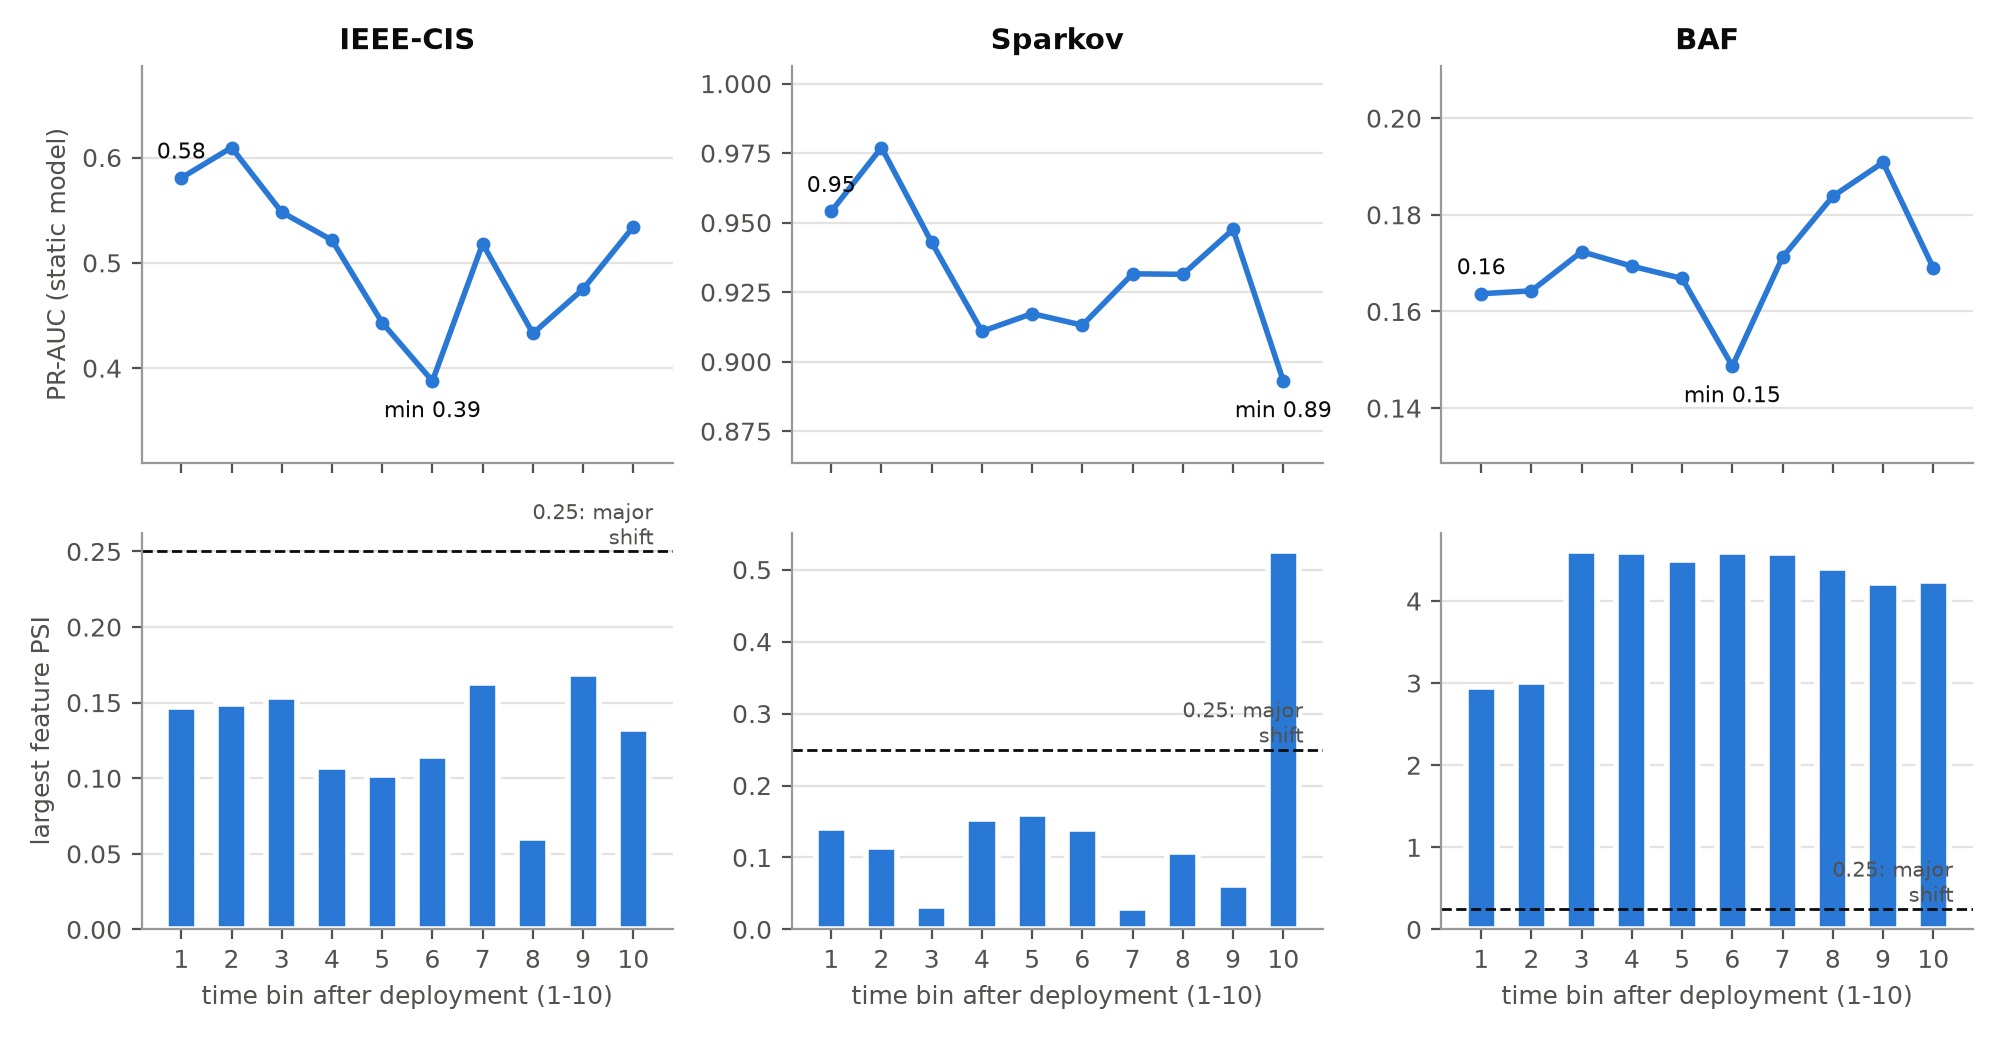
\includegraphics[width=0.95\textwidth]{figures/results_decay.png}
  \caption*{Figure 5.1: Static model after deployment, in ten consecutive time bins of the test period: PR-AUC (top) and the largest PSI among the ten most important features (bottom). Each panel has its own scale}
\end{figure}

The drift measures do not perceive it and the IEEE-CIS decays. The PR-AUC of the static model decreased from 0.581 in the first time bin to 0.388 in the sixth, a third of the way, before recovering somewhat to 0.534. The identical bins had their ROC-AUC reduced from 0.920 to 0.849. In the same period none of the ten most essential features scored a major shift (the largest PSI was 0.17) and the PSI of the scores of the model never exceeded 0.017. This implies that a label-free monitor would have seen a stable system at the time of the greatest drop in performance in the study. This accords with the decay found by Menezes and Filho for graph models on the same data set [4], and shows that the decay is not observable in the input distribution.

\textbf{No deterioration in the model of Sparkov and BAF drift.} On Sparkov, the per-card activity features had a significant drift in the last bin (PSI 0.53), and on BAF, the velocity features shifted above any normal threshold in all bins (PSI up to 4.60), while the PR-AUC remained in the range 0.89-0.98 on Sparkov, and 0.15-0.19 on BAF, with no negative trend. A drift monitor on these features would have gone off virtually weekly. The score-PSI trigger, which looks at the outputs of the model, not the inputs, fired only once on Sparkov, at one of the four label delays, and never on BAF.

\textbf{Answer to RQ1:} Performance of a deployed fraud model can decay dramatically. If it does depends on the data. Label-free drift metrics are not a reliable predictor of this in any direction: they missed true decay on IEEE-CIS and detected drift that did not matter on Sparkov and BAF. This is the case that Shakil et al. when they stated that statistical drift is not always associated with lower performance [1] currently shown on natural drift in fraud data.

\subsection*{5.1.4\quad Retraining under Label Delay}
\addcontentsline{toc}{subsection}{5.1.4\quad Retraining under Label Delay}

Table 5.2 and Figure 5.2 compare scheduled retraining every 14 days with the static model at label delays of 0, 15, 30 and 60 days.

\begin{center}\small Table 5.2: Gain in mean weekly PR-AUC over the static model by label delay (retraining every 14 days; 95\% intervals)\end{center}
\vspace{-1.2em}

{\small
\begin{longtable}{|>{\raggedright\arraybackslash}p{0.109\textwidth}|>{\raggedright\arraybackslash}p{0.184\textwidth}|>{\raggedright\arraybackslash}p{0.109\textwidth}|>{\raggedright\arraybackslash}p{0.169\textwidth}|>{\raggedright\arraybackslash}p{0.162\textwidth}|>{\raggedright\arraybackslash}p{0.147\textwidth}|}
\hline
Dataset & Delay & Static & All history & Last 60 days & Drift: performance \\ \hline
IEEE-CIS & 0 d & 0.507 & +0.033 [0.027, 0.040] & +0.078 [0.067, 0.088] & +0.030 (2 retrains) \\ \hline
 & 15 d & 0.491 & +0.025 [0.020, 0.029] & +0.062 [0.052, 0.072] & +0.020 (2) \\ \hline
 & 30 d & 0.474 & +0.028 [0.022, 0.033] & +0.056 [0.046, 0.064] & +0.027(3) \\ \hline
 & 60 d & 0.472 & +0.008 [0.002, 0.014] & +0.010 [0.004, 0.016] & +0.010 (4) \\ \hline
Sparkov & 0 d & 0.931 & +0.016 [0.013, 0.020] & -0.258 [-0.273, -0.242] & 0 \\ \hline
 & 15 d & 0.928 & +0.017 [0.013, 0.021] & -0.214 [-0.228, -0.199] & 0 \\ \hline
 & 30 d & 0.924 & +0.019 [0.016, 0.023] & -0.173 [-0.187, -0.160] & 0 \\ \hline
 & 60 d & 0.923 & +0.019 [0.015, 0.023] & -0.198 [-0.211, -0.183] & 0 \\ \hline
BAF & 0 d & 0.162 & +0.011 [0.007, 0.015] & -0.003 [-0.007, 0.002] & 0 \\ \hline
 & 15 d & 0.161 & +0.008 [0.004, 0.012] & -0.005 [-0.011, 0.000] & 0 \\ \hline
 & 30 d & 0.161 & +0.009 [0.004, 0.014] & -0.007 [-0.013, -0.002] & 0 \\ \hline
 & 60 d & 0.155 & +0.010 [0.006, 0.015] & +0.002 [-0.003, 0.007] & +0.001 (1) \\ \hline
\end{longtable}
}

\begin{figure}[H]
  \centering
  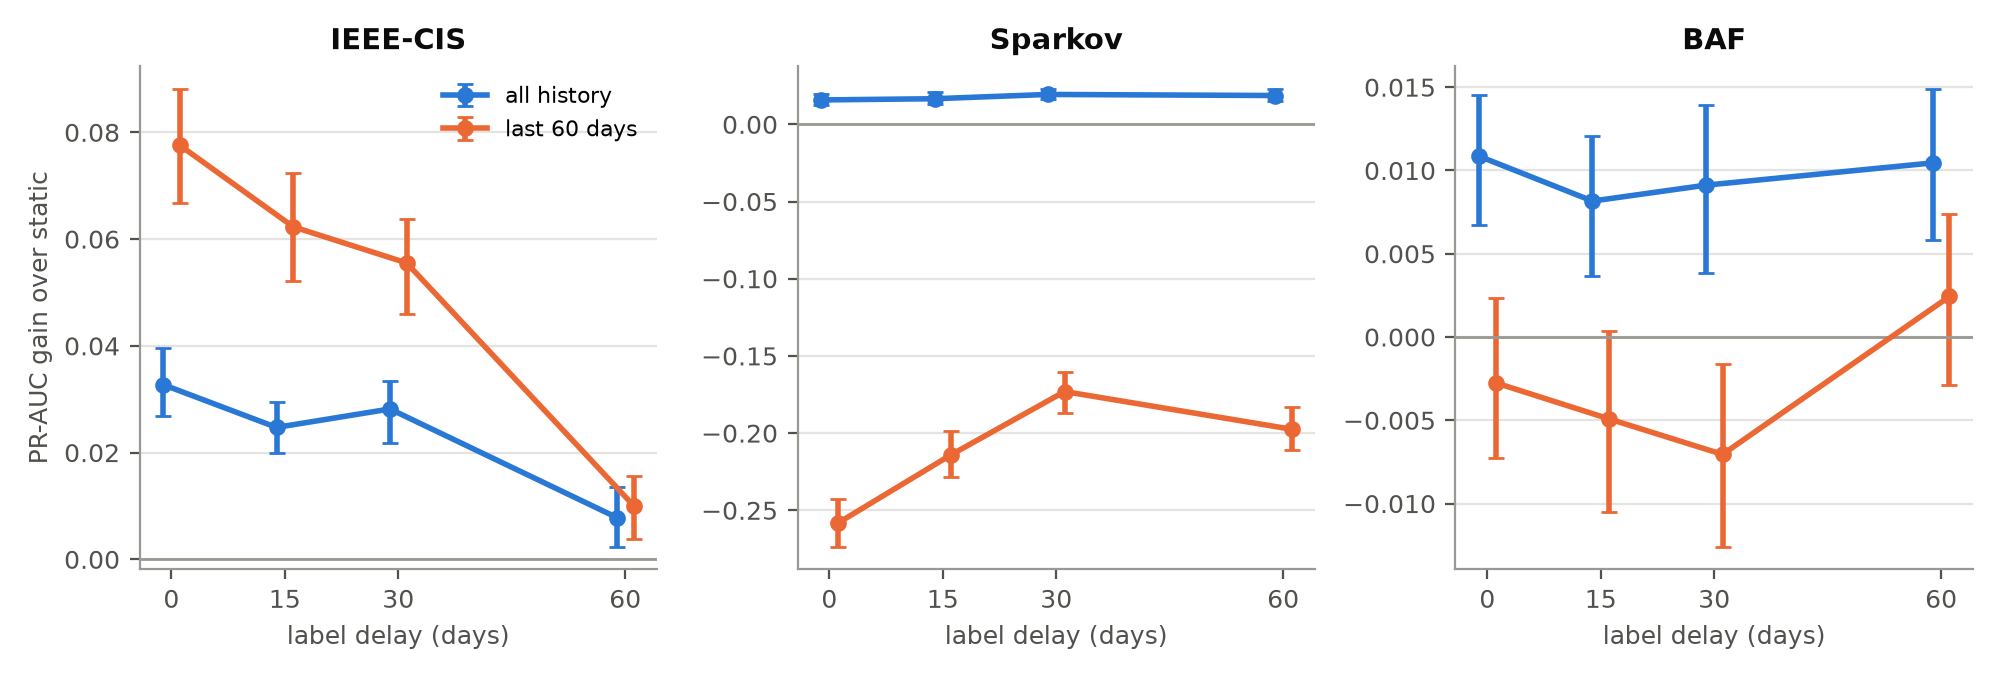
\includegraphics[width=0.95\textwidth]{figures/results_delay.png}
  \caption*{Figure 5.2: Gain in mean weekly PR-AUC over the static model for scheduled retraining every 14 days, by label delay, with 95\% paired bootstrap intervals}
\end{figure}

\textbf{Retraining does help when its window matches the data}: On IEEE-CIS both windows improved on the static model at every delay, and the latest 60 days was clearly better than total history (+0.078 against +0.033 at no delay). On Sparkov and BAF, the sequence reversed: retraining on all history gave +0.016 to +0.019 and +0.008 to +0.011 at each delay, at each interval except zero, whereas the 60-day window was worse than not retraining at all, drastically so on Sparkov (-0.17 to -0.26). Sparkov has a consistent fraud pattern with only 0.53\% fraud: there are too few frauds in 60 days to relearn and the model does not benefit from forgetting prior data. IEEE-CIS, in contrast, is drifting, and older data teaches the model patterns that no longer apply.

\textbf{Failure to label on time means loss of benefit:} On IEEE-CIS the gain of the 60-day window dropped from +0.078 with instantaneous labels to +0.062 at 15 days, +0.056 at 30 days and +0.010 at 60 days, while the static model itself decreased just from 0.507 to 0.472. A retrained model learns from data that is two months old, which on a drifting dataset is no better than the initial training data, with 60 days of delay. On Sparkov and BAF the gain of all-history retraining scarcely changes with delay, consistent with their non-decay: when the pattern is stable, old labels are still relevant.

\textbf{Untuned drift triggers seldom act:} The performance trigger retrained two to four times on IEEE-CIS with default settings and achieved between a third and half of the gain of the 60-day schedule with delays up to 30 days. On Sparkov and BAF it nearly never fired, as performance never fell 15\% and it behaved like the static model. Answer to RQ2. Retraining increased performance on all datasets, but only with a training window appropriate for the data, and on the drifting dataset its benefit decreased rapidly as labels arrived later; at 60 days of delay most of the benefit was lost. This validates, using public data, the impact of verification latency pointed forth by Dal Pozzolo et al. [5].

\section*{5.2\quad Analyse Design Solutions}
\addcontentsline{toc}{section}{5.2\quad Analyse Design Solutions}

\subsection*{5.2.1\quad Drift-Triggered versus Scheduled Retraining}
\addcontentsline{toc}{subsection}{5.2.1\quad Drift-Triggered versus Scheduled Retraining}

The comparison in Section 5.1.4 used default settings. Table 5.3 gives the fair comparison: every family was re-tuned every four weeks with walk-forward tuning over 190 configurations, using only labels that had matured at the time

{\small
\begin{longtable}{|>{\raggedright\arraybackslash}p{0.117\textwidth}|>{\raggedright\arraybackslash}p{0.109\textwidth}|>{\raggedright\arraybackslash}p{0.124\textwidth}|>{\raggedright\arraybackslash}p{0.135\textwidth}|>{\raggedright\arraybackslash}p{0.222\textwidth}|>{\raggedright\arraybackslash}p{0.173\textwidth}|}
\hline
Dataset & Delay & Static & Schedule-(retr ains) & Schedule -static & Drift trigger-schedule \\ \hline
IEEE-CIS & 0 d & 0.470 & 0.614 (12) & +0.144 [0.132, 0.158] & 0.069 [-0.082, -0.060] \\ \hline
 & 15 d & 0.468 & 0.547 (12) & +0.079 [0.070, 0.091] & -0.034 [-0.044, -0.027] \\ \hline
 & 30 d & 0.458 & 0.518 (6) & +0.059 [0.049, 0.069] & -0.032 [-0.038, -0.025] \\ \hline
Sparkov & 0 d & 0.916 & 0.945 (12) & +0.029 [0.024, 0.033] & -0.001 [-0.003, 0.001] \\ \hline
 & 15 d & 0.913 & 0.944 (12) & +0.031 [0.026, 0.036] & -0.007 [-0.010, -0.004] \\ \hline
 & 30 d & 0.917 & 0.943 (12) & +0.027 [0.023, 0.031] & -0.007 [-0.009, -0.004] \\ \hline
BAF & 0 d & 0.163 & 0.174 (8) & +0.011 [0.006, 0.016] & -0.011 [-0.016, -0.006] \\ \hline
 & 15 d & 0.157 & 0.168 (8) & +0.011 [0.007, 0.016] & -0.006 [-0.011, -0.002 \\ \hline
 & 30 d & 0.159 & 0.162 (7) & +0.003 [-0.003, 0.008] & +0.001 [-0.003, 0.006] \\ \hline
\end{longtable}
}

\begin{center}\small Table 5.3: Walk-forward tuning: each family re-tuned every four weeks on matured labels only (mean weekly PR-AUC, total retrains, and differences with 95\% intervals)\end{center}
\vspace{-1.2em}

\textbf{The tuned schedule was better than or equal to the tuned trigger everywhere.} The schedule was better than the drift trigger on IEEE-CIS by 0.069, 0.034 and 0.032 PR-AUC at delays 0, 15 and 30 days, all dependable. The trigger was quite close on Sparkov with many fewer retrains (12 vs. 2 to 8). The gap was within noise with immediate labels and 0.007 at 15 and 30 days.

The schedule was superior at 0 and 15 days on BAF and at 30 days neither retraining family was reliably better than the static model as gains on BAF are minimal. The trigger was reliably worse in seven of the nine comparisons, and never reliably better. The behaviour of the tuned trigger under label delay is observed as the reason. It can only respond to a drop in performance once the drop has been validated by labels that are at least one delay old, and a dip has to exceed noise in weekly PR-AUC before it is acted upon. The schedule keeps the model fresh without waiting for evidence. Where the trigger got near, like in Sparkov, it did so by infrequently retraining on a stable dataset where retraining matters little.

\textbf{Answer to RQ3:} No. Drift-triggered retraining did not beat scheduled retraining on any of the three datasets when both were reasonably calibrated and labels were late; it was worse in most comparisons and at best equal, albeit it retrained less often. This is contrary to the results of Wong and Perumal [2] and Yelleti [3] for injected drift or instantaneous labelling. The choice of training window had a larger influence than the choice of trigger, changing the result by up to 0.26 PR-AUC.

\subsection*{5.2.2\quad Equal-Budget Comparison}
\addcontentsline{toc}{subsection}{5.2.2\quad Equal-Budget Comparison}

Scheduled retraining retrained more often than the drift triggers in the comparisons above (e.g. 12 against 2 to 5 retrains in walk-forward tuning on IEEE-CIS), so part of its advantage could come simply from retraining more regularly. To separate the two, we ran both families over many settings on IEEE-CIS and BAF, schedules every 7 days or more, and 64 trigger settings. Each trigger setting was paired with the schedule that uses the same training window and the largest number of retrains that does not exceed the trigger's. Therefore the schedule never has more retrains than the trigger it is being compared with, which biases in favour of the trigger. The pairs are summarised in Table 5.4 and Figure 5.3 displays the best PR-AUC each family gets within a particular budget.

{\small
\begin{longtable}{|>{\raggedright\arraybackslash}p{0.110\textwidth}|>{\raggedright\arraybackslash}p{0.110\textwidth}|>{\raggedright\arraybackslash}p{0.110\textwidth}|>{\raggedright\arraybackslash}p{0.110\textwidth}|>{\raggedright\arraybackslash}p{0.107\textwidth}|>{\raggedright\arraybackslash}p{0.110\textwidth}|>{\raggedright\arraybackslash}p{0.110\textwidth}|>{\raggedright\arraybackslash}p{0.110\textwidth}|}
\hline
Dataset & Delay & Window & Pairs & Schedule better (reliability ) & Trigger reliably better & Mean diff. & Retrains \\ \hline
IEEE-CIS & 0 d & Last 60 days & 27 & 18(9) & 0 & +0.016 & 1.7/1.7 \\ \hline
 & 30 d & Last 60 days & 30 & 23 (7) & 0 & +0.011 & 2.2/2.2 \\ \hline
 & 0 d & All history & 28 & 15 (14) & 0 & +0.005 & 1.7/1.6 \\ \hline
 & 30 d & All history & 30 & 12 (0) & 0 & 0.000 & 2.3/2.2 \\ \hline
BAF & 0 d & Last 60 days & 9 & 9 (2) & 0 & +0.003 & 2.2/2.2 \\ \hline
 & 30 d & Last 60 days & 0 & - & 0 & - & Trigger never fired \\ \hline
 & 0 d & All history & 10 & 2 (1) & 0 & -0.002 & 1.9/1.9 \\ \hline
 & 30 d & All history & 2 & 2 (1) & 0 & +0.004 & 2.5/2.5 \\ \hline
\end{longtable}
}

\begin{center}\small Table 5.4: Equal-budget comparison: each trigger setting paired with the schedule that uses the same window and no more retrains (95\% intervals; retrains: trigger / schedule)\end{center}
\vspace{-1.2em}

\begin{figure}[H]
  \centering
  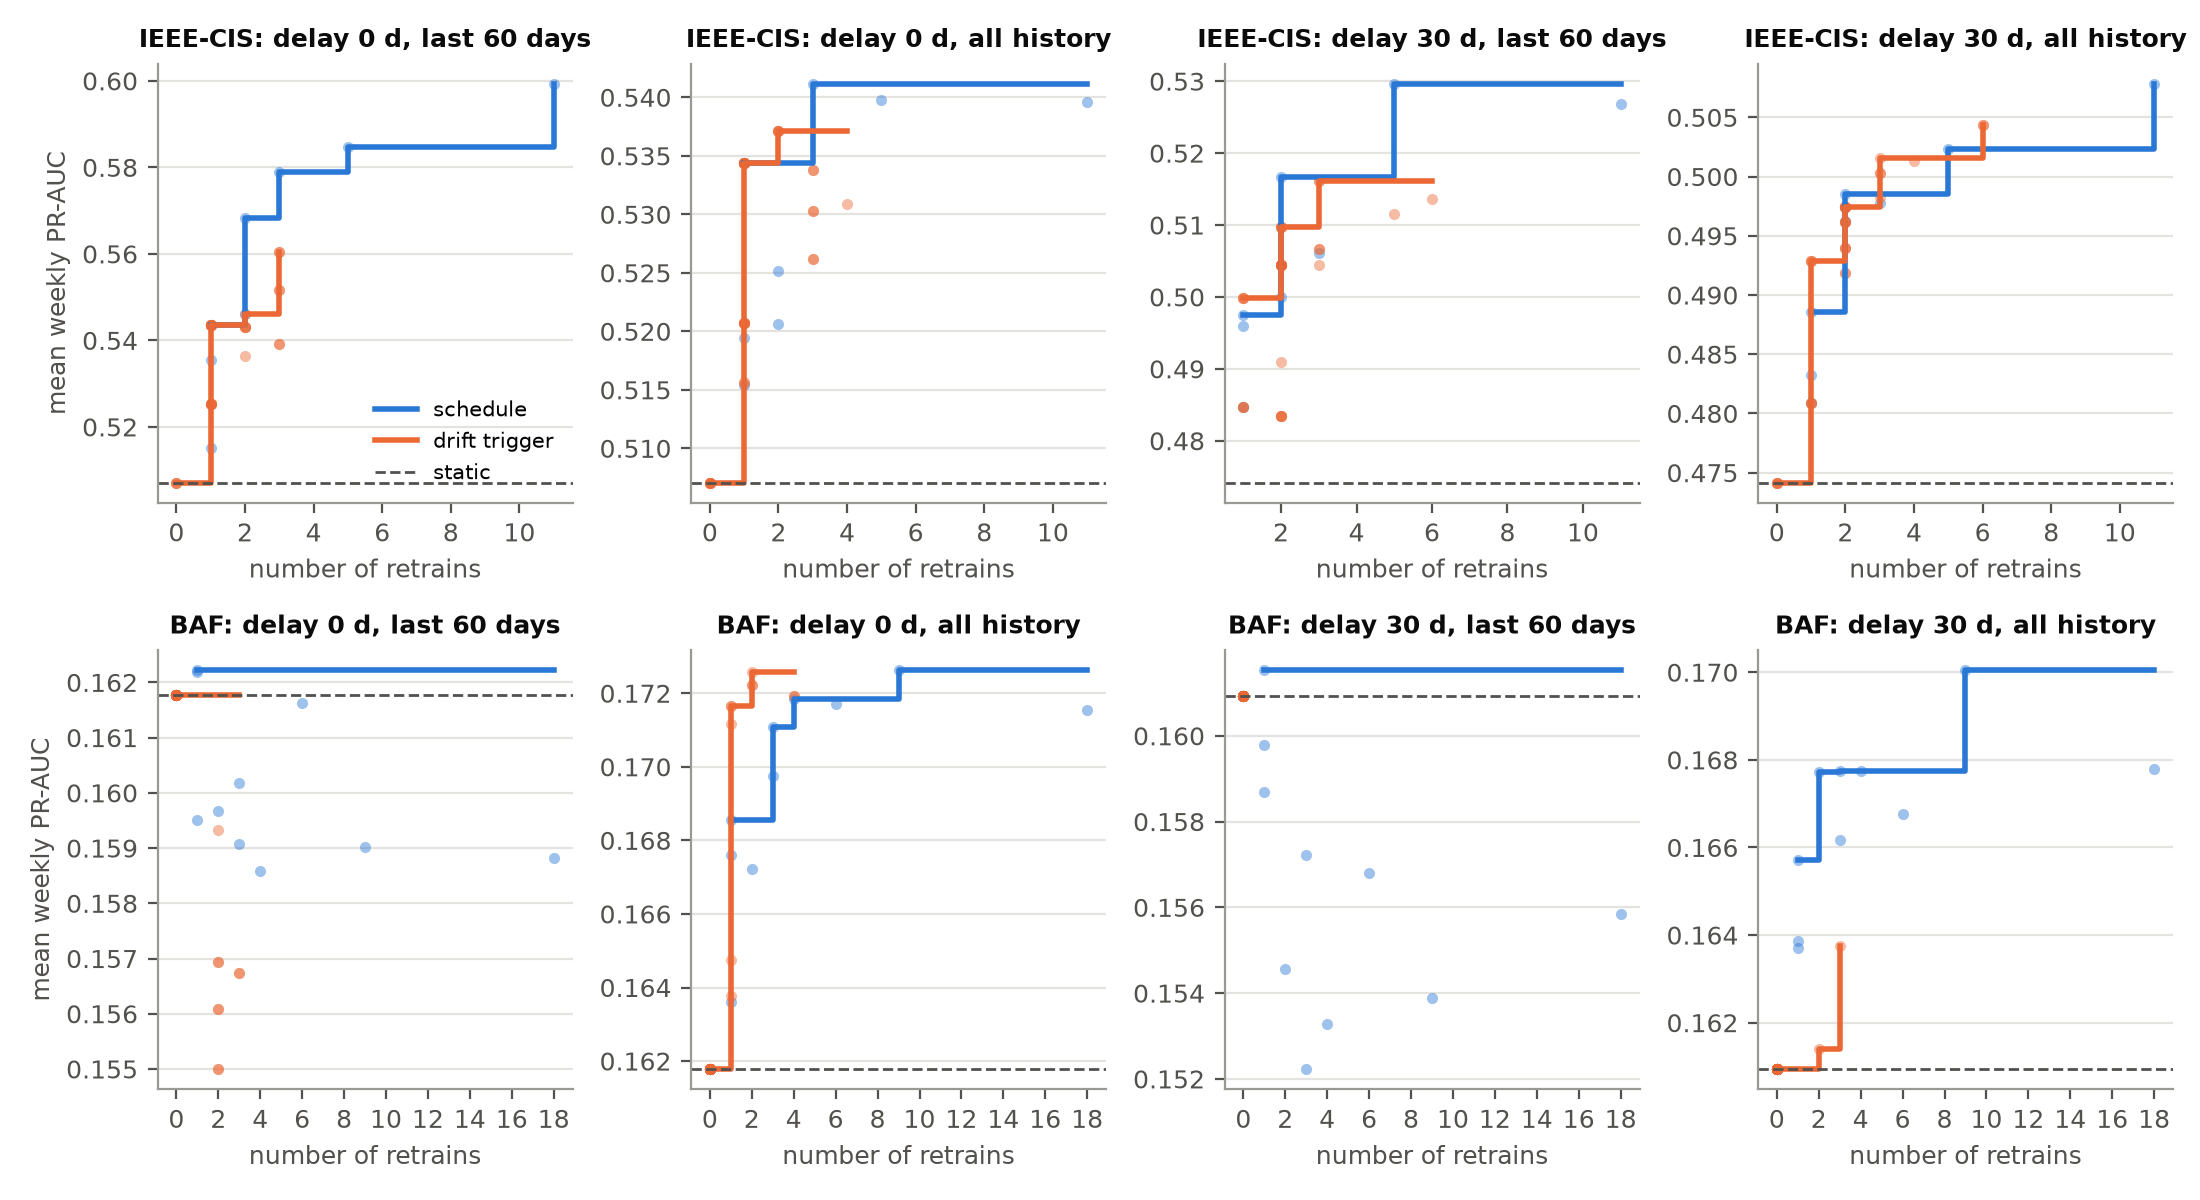
\includegraphics[width=0.95\textwidth]{figures/results_equal_budget.png}
  \caption*{Figure 5.3: Equal-budget comparison on IEEE-CIS (top) and BAF (bottom): the best mean weekly PR-AUC each family reaches with at most a given number of retrains (dots: individual settings)}
\end{figure}

The schedule was better in 18 of 27 pairs with immediate labels and 23 of 30 pairs at a 30 day delay, reliably so in 9 and 7 pairs, and the trigger was never reliably better. On average the schedule was 0.016 and 0.011 PR-AUC ahead at the same budget. For example, with two retrains the best schedule was 0.568 and the best trigger was 0.546. The two were close with full history as training data: schedule was ahead by 0.005 with immediate labels and level at a 30 day lag.

The label-free score-PSI trigger fired only once in all settings. Finally, the triggers required only two or three retrains most of the time, while the schedule kept improving with more frequent retrains (0.599 with eleven retrains).

The triggers scarcely fired on BAF at all, since the performance little altered; most settings never retrained and no setting with the 60-day window fired with a 30-day lag. In the presence of pairings, the picture depends on the label delay. When trained with immediate labels and full history, the trigger was the cheaper policy: it was consistently better than the other in 3 out of 10 pairs, and its best setting was 0.173 with 2 retrains, which the schedule only matched with 9. All 9 pairs had an improved schedule with the 60-day window. At a realistic 30-day lag the schedule was ahead again: with two retrains it reached 0.168 vs. 0.161 for the best trigger, and 0.170 vs. 0.164 at best.

So the advantage of scheduled retraining is not merely about retraining more often. When labels were delayed by 30 days, the schedule matched or beat the drift trigger at an equal budget on both datasets, and was never reliably poorer on IEEE-CIS. A trigger can be cheap when labels arrive quickly as on BAF with entire history, consistent with prior work that assumed immediate labels [3]. Under label delay it has to wait for evidence of degradation and loses that benefit. Another contribution to the overall advantage of the schedule is the larger number of retrains, which cannot be achieved by a delayed-label trigger. The comparison on Sparkov is done the same manner.

\subsection*{5.2.3\quad Framework Replay}
\addcontentsline{toc}{subsection}{5.2.3\quad Framework Replay}

Replay. We execute four window settings on the same Kaggle machine. Table 5.5 provides the framework repeated across the stream of each dataset with 30-day label delay. The framework nearly duplicated the offline simulation of the identical policy: 0.529 vs. 0.530 for the 60-day window on IEEE-CIS, 0.942 vs. 0.943 for full history on Sparkov, and 0.169 vs. 0.170 on BAF. An previous replay of the default configuration on a desktop computer gave 0.531 on [IEEE-CIS]. So the MLOps components from the registry, to the promotion gate, to the monitoring loop, add their protections, without impacting the performance of the policy they run.

{\small
\begin{longtable}{|>{\raggedright\arraybackslash}p{0.222\textwidth}|>{\raggedright\arraybackslash}p{0.218\textwidth}|>{\raggedright\arraybackslash}p{0.222\textwidth}|>{\raggedright\arraybackslash}p{0.218\textwidth}|}
\hline
 & IEEE-CIS (12 weeks) & Sparkov (52 weeks) & BAF (19 weeks) \\ \hline
Static model & 0.478 & 0.924 & 0.161 \\ \hline
Last 60 days & 0.529(5,0) & 0.752 (26, 11) & 0.153 (9,0) \\ \hline
All history & 0.504(6,0) & 0.942 (25,0) & 0.169 (9,1) \\ \hline
Automatic window & 0.529 (5,0) & 0.942 (25, 1) & 0.165 (9,1) \\ \hline
Window chosen & 60 days in 5 of 5 & All history in 25 of 25 & All history in 7 of 9 \\ \hline
Official simulation: last 60 days/ all history & 0.530/0.502 & 0.751/0.943 & 0.154/0.170 \\ \hline
\end{longtable}
}

\begin{center}\small Table 5.5: Framework replays at a 30-day label delay: mean weekly PR-AUC (retrains, rejected by the gate) and the offline simulation of the same policy\end{center}
\vspace{-1.2em}

\subsection*{5.2.4\quad Safeguards under Fault Injection}
\addcontentsline{toc}{subsection}{5.2.4\quad Safeguards under Fault Injection}

Fault Injection Protection. Figure 5.4 and Table 5.6 illustrates the IEEE-CIS replay with two failed retraining jobs. The promotion gate rejected all 6 faulty models generated from training-job faults. The shuffled labels generated PR-AUCs of 0.035, no better than chance, and the label outage gave 0.275 and 0.445 vs champions of 0.475 and 0.620. The hardest example was the feature unit bug, which models scored 0.464 and 0.597 vs. 0.475 and 0.620, and were rejected only because they were re-scored on production features and slipped slightly outside the tolerance of 0.01. With the gate on each of these three errors cost 0.012 PR-AUC, the price of keeping an older champion for two weeks. Without the gate defective models were promoted and cost was increased to 0.019, 0.039 and 0.080.

{\small
\begin{longtable}{|>{\raggedright\arraybackslash}p{0.178\textwidth}|>{\raggedright\arraybackslash}p{0.102\textwidth}|>{\raggedright\arraybackslash}p{0.170\textwidth}|>{\raggedright\arraybackslash}p{0.178\textwidth}|>{\raggedright\arraybackslash}p{0.253\textwidth}|}
\hline
Fault & Gate & Mean PR-AUC & Change vs clean & Faulty models promoted \\ \hline
None (clean) & on & 0.531 & - & - \\ \hline
Label shuffle & on & 0.519 & -0.012 & 0 of 2 (0.035 vs 0.475; 0.034 vs 0.620) \\ \hline
 & off & 0.451 & -0.080 & 2 of 2 \\ \hline
Label loss (80\%) & on & 0.519 & -0.012 & 0 of 2 (0.275 vs 0.475; 0.445 vs 0.620) \\ \hline
 & off & 0.492 & -0.039 & 2 of 2 \\ \hline
Feature unit bug & on & 0.519 & -0.012 & 0 of 2 (0.464 vs 0.475; 0.597 vs 0.620) \\ \hline
 & off & 0.512 & -0.019 & 2 of 2 \\ \hline
Upstream label shuffle & on & 0.451 & -0.080 & 2 of 2; safety net replaced each after 7 days \\ \hline
 & off & 0.451 & -0.080 & 2 of 2 \\ \hline
\end{longtable}
}

\begin{center}\small Table 5.6: Fault injection on IEEE-CIS (two faulty retraining jobs, 30-day label delay)\end{center}
\vspace{-1.2em}

\begin{figure}[H]
  \centering
  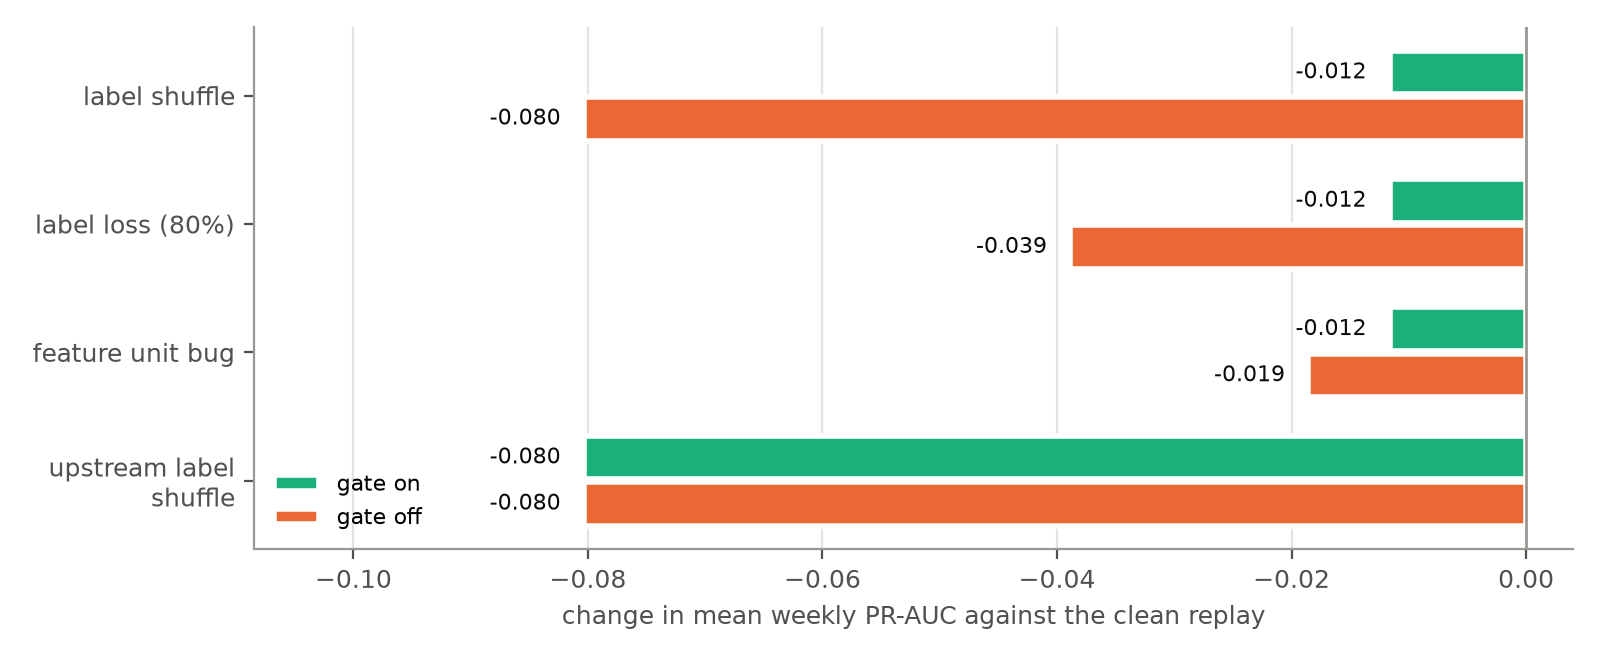
\includegraphics[width=0.95\textwidth]{figures/results_gate.png}
  \caption*{Figure 5.4: Fault injection on IEEE-CIS: change in mean weekly PR-AUC against a clean replay when two retraining jobs are faulty, with the promotion gate on and off}
\end{figure}

Since both models looked equally bad on corrupted labels , the gate itself reads the label store , which is contaminated . The upstream fault that corrupts the label store passed the gate as expected . Here the safety net kicked in: seven days after each bad promotion the live PR-AUC on matured labels had dropped to 0.045 and 0.036, below both 70\% of the reference and three times the fraud rate and the framework retrained early. The harm was confined to one week per defect (-0.080 overall). Prior to the safety net reference to recent live performance (Section 4.2.4), the same problem was missed and cost -0.149.

\textbf{Answer to RQ4:} Yes. The framework retained the performance of the best offline policy in a full replay, prevented every faulty model it could see from going into production, recovered within a week from the fault it could not see, and with automatic window selection, performed at or near the best fixed window on all three dataset, based on the results of RQ1 to RQ3.

\section*{5.3\quad Final Design Adjustments}
\addcontentsline{toc}{section}{5.3\quad Final Design Adjustments}

Three changes were made to the design during the evaluation, each prompted by a result.

\subsection*{5.3.1\quad Promotion Gate on Production Features}
\addcontentsline{toc}{subsection}{5.3.1\quad Promotion Gate on Production Features}

The original version of the promotion gate compared the challenger and champion based on scores that were stored while each model was trained. A feature unit defect, a fault test, revealed the fragility of this: a model trained on improperly scaled features appears good on similarly bad validation data. The gate was re-designed to re-score both models along the production feature path (Section 4.2.6) and then reject the incorrect models.

\subsection*{5.3.2\quad Safety-Net Reference from Live Performance}
\addcontentsline{toc}{subsection}{5.3.2\quad Safety-Net Reference from Live Performance}

Initially the safety net contrasted the model's own validation PR-AUC with the real PR-AUC. So went unnoticed, costing 0.149 PR-AUC. When the label store itself was corrupted, a bad model reporting a bad validation score was scored against that low bar. A no-skill check was added (Section 4.2.4) and the reference was modified to the best of the validation score and the median of the last four live measures. The same problem was identified after seven days and cost 0.080.

\subsection*{5.3.3\quad Automatic Training-Window Selection}
\addcontentsline{toc}{subsection}{5.3.3\quad Automatic Training-Window Selection}

Automatic selection of training windows. There was no one optimal fixed window across all three datasets: the 60-day window was best on IEEE-CIS (0.529), but lost by 0.172 to the static model on Sparkov; full history was best on Sparkov and BAF, but only second on IEEE-CIS. The framework with automatic selection selected the 60-day window at all five retrains on IEEE-CIS and full history at all 25 retrains on Sparkov, which was the same as the best fixed window on both (difference of 0.000 and -0.0002). On BAF it chose the 60-day window on the first two retrains when the two candidates were close and the shorter window scored somewhat better on recent data, and all history on the rest of the seven. It was 0.0045 less than the best fixed window on BAF, a tiny but reliable difference (95\% CI across weeks -0.008 to -0.001) and 0.004 over the static model. The automatic setup prevented the substantial loss of a bad window choice on every dataset without knowing in advance which window was suitable for the data as shown in Figure 5.5.

\begin{figure}[H]
  \centering
  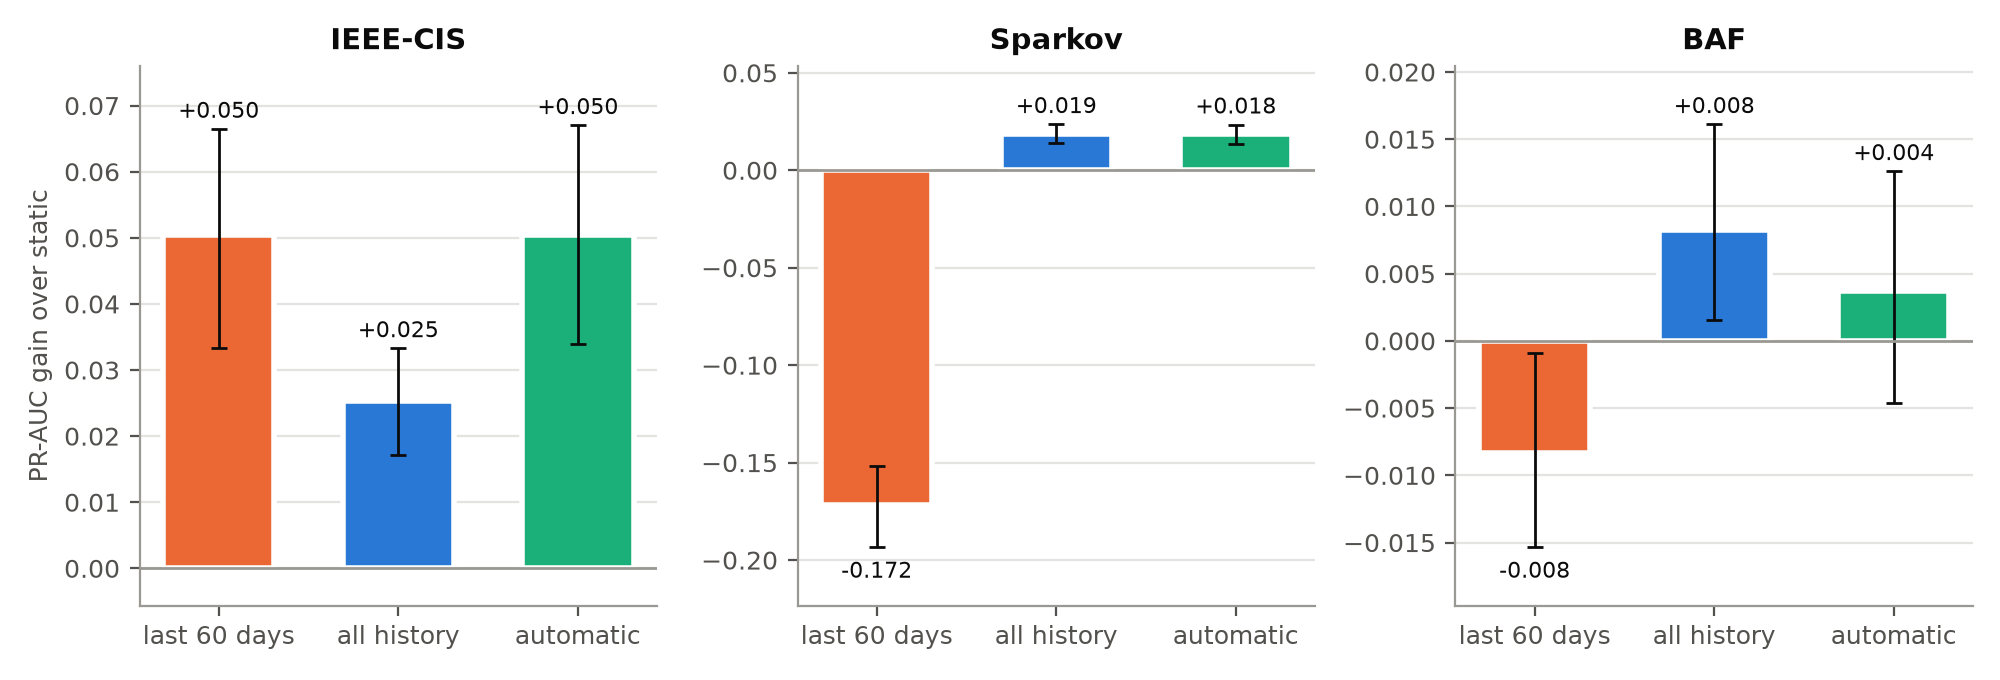
\includegraphics[width=0.95\textwidth]{figures/results_window.png}
  \caption*{Figure 5.5: Framework replays (30-day label delay): gain in mean weekly PR-AUC over the static model for each training-window choice, with 95\% bootstrap intervals over weeks}
\end{figure}

\section*{5.4\quad Summary of Results}
\addcontentsline{toc}{section}{5.4\quad Summary of Results}

Table 5.7 highlights the replies to the research questions. Overall, the results validate the design of the proposed framework: performance is monitored on delayed labels rather than inferred from drift, retraining follows a schedule rather than a drift alarm, the training window is selected from the data, and every new model must pass a promotion gate. In section 5.6 we address the implications of these results, their relation to previous work and their limitations.

{\small
\begin{longtable}{|>{\raggedright\arraybackslash}p{0.124\textwidth}|>{\raggedright\arraybackslash}p{0.756\textwidth}|}
\hline
RQ & Answer \\ \hline
RQ1 & Performance after deployment changed differently on each dataset: it fell by a third on IEEE-CIS but stayed stable on Sparkov and BAF. Label-free drift measures did not reflect this: input and score drift stayed low while IEEE-CIS decayed, and input drift was strong (PSI up to 4.6) while Sparkov and BAF did not. \\ \hline
RQ2 & Scheduled retraining improved performance on every dataset when its window suited the data, with gains of 0.008 to 0.078 PR-AUC. On IEEE-CIS the gain shrank from 0.078 to 0.010 as the label delay grew from 0 to 60 days. \\ \hline
RQ3 & No. Tuned fairly with walk-forward tuning, drift-triggered retraining was worse than scheduled retraining in 7 of 9 comparisons and never better beyond noise; it retrained less often. The training window mattered more than the trigger. \\ \hline
RQ4 & Yes. The framework reproduced the offline results within 0.002 PR-AUC, blocked every faulty model the gate could observe, limited the damage of the unobservable fault through the safety net, and, with automatic window selection, matched the best fixed \\ \hline
 & window on two datasets and came within 0.005 on the third. \\ \hline
\end{longtable}
}

\begin{center}\small Table 5.7: Answers to the research questions\end{center}
\vspace{-1.2em}

Three levels of statistical analysis back up the findings. First, we pair each comparison between strategies: all strategies are evaluated on the same weeks and the same bootstrap resamples, removing most of the noise they share. Second, the paired day-block bootstrap resamples entire days within each week, observing the correlation between transactions of the same day, and returns the 95\% intervals stated throughout. Third, we deal with the randomness of training by repeating the crucial comparisons with five LightGBM seeds.

{\small
\begin{longtable}{|>{\raggedright\arraybackslash}p{0.177\textwidth}|>{\raggedright\arraybackslash}p{0.173\textwidth}|>{\raggedright\arraybackslash}p{0.177\textwidth}|>{\raggedright\arraybackslash}p{0.173\textwidth}|>{\raggedright\arraybackslash}p{0.179\textwidth}|}
\hline
Dataset & Delay & All history-static & Last 60 days-static & Default drift trigger-best schedule \\ \hline
IEEE-CIS & 0 d & +0.033 (5/5) & +0.080 (5/5) & -0.055 (0/5) \\ \hline
 & 30 d & +0.022 (5/5) & +0.046 (5/5) & -0.026 (0/5) \\ \hline
Sparkov & 0 d & +0.012 (5/5) & -0.194 (0/5) & -0.012 (0/5) \\ \hline
 & 30 d & +0.016 (5/5) & -0.171 (0/5) & -0.016 (0/5) \\ \hline
BAF & 0 d & +0.006 (5/5) & -0.006 (0/5) & -0.006 (0/5) \\ \hline
 & 30 d & +0.009 (5/5) & -0.007 (0/5) & -0.009 (0/5) \\ \hline
\end{longtable}
}

\begin{center}\small Table 5.8: Key differences over five training seeds (mean, and the number of seeds in which the difference is positive). Best schedule: last 60 days on IEEE-CIS, all history on Sparkov and BAF\end{center}
\vspace{-1.2em}

\textbf{The results are not attributable to randomness in training.} In table 5.8 we again show the key comparisons with five lightgbm seeds. All the differences in the table had the same sign for all the five seeds for each dataset. The variation of a single configuration over seeds was minor compared to the variation between strategies: the median standard deviation was 0.004 on IEEE-CIS, 0.010 on Sparkov and 0.003 on BAF. Many comparisons are presented and a single interval excluding zero should not be over-interpreted. Instead this thesis's conclusions are based on patterns that hold across label delays, datasets, seeds and analyses. For example, the drift trigger was reliably worse than the schedule in seven out of nine walk-forward comparisons and never reliably better in any of them, and the equal-budget analysis pointed the same way whenever labels were delayed.

\section*{5.6\quad Discussions}
\addcontentsline{toc}{section}{5.6\quad Discussions}

\textbf{Delayed labels and drift indications:} The main finding was that the label-free drift indicators did not reflect what counted. They remained silent when the IEEE-CIS model lost a third of its PR-AUC, and they showed substantial drift on Sparkov and BAF while the models were unaffected. Shakil et al. point out that statistical drift does not always equal inferior performance [1], and we saw this for both directions of natural drift in fraud data. In a fraud system, it implies drift alerts should inform inquiry, not trigger retraining, and performance on matured labels is the signal to watch, even if it arrives late. In this way the framework knows about the drift.

\noindent\textbf{Timetables and triggers Previous work has shown that drift-triggered retraining performs as well}

\textbf{as or better than a schedule with fewer retrains [2], [3]}. Those outcomes were achieved using injected drift or instantaneous labels A performance trigger under realistic label delay can only react after drop confirmation on weeks-old labels, while a label-free trigger reacts to the wrong signal. A timetable is evidence-free, and keeps the model fresh, with the equal-budget analysis showing that its advantage under label delay is not just retraining more regularly. The more economical strategy might be a trigger with instant labels as on BAF, which is why previous studies that assumed immediate labels supported triggers. This is in agreement with Dal Pozzolo et al. who pointed out the relevance of the verification latency for the updating of a fraud model [5] and with Amekoe et al. who noted that the batch models re-trained on delayed labels were still competitive [11].

\textbf{Training time:} The choice of training window affected the findings by up to 0.26 PR-AUC, far more than the choice of trigger. The latest data performed best on the volatile dataset IEEE-CIS, whereas the entire history performed best on the stable datasets Sparkov and BAF, which contain few frauds. No predefined window is suitable for all deployments. Identifying the window from the data as the framework does today is a practical approach of avoiding an expensive wrong choice.

\textbf{Secure automation:} Automated retraining eventually will train on faulty data. The fault tests indicate that a promotion gate that re-scores models on production data stops errors it can see, and that a safety net based on live performance lowers the damage of faults it cannot. Closed-loop MLOps frameworks like HAMF [17] automate the loop; this thesis provides evidence on how such protections behave when labels arrive late.

\textbf{Restrictions:} The deployment is replayed from previous data so we can not see live latency and the behaviour of a real chargeback feed, and every label arrives after the same wait, without faster investigator feedback. The same family of models is used throughout. IEEE-CIS only lasts six months, Sparkov is simulated, and BAF only records the month of each application, thus drift within a month cannot occur. The equal-budget comparison is completed on IEEE-CIS and BAF, in progress on Sparkov and the scoring service is still to be load tested.

\setcounter{chapter}{5}
\chapter{Conclusion}

\section*{6.1\quad Summary of Results}
\addcontentsline{toc}{section}{6.1\quad Summary of Results}

In this thesis, we aimed at designing and evaluating a drift-aware continuous learning MLOps framework for financial transaction fraud detection that can determine whether a deployed model is getting obsolete, when to retrain the model and deploy a new and better model in a safe manner. We replayed three public datasets with realistic label delay and obtained five main findings:

\listitem{1. Label-free drift indicators did not represent model performance: they missed a loss of a third of the PR-AUC on IEEE-CIS and signalled strong drift on Sparkov and BAF, where performance did not drop.}

\listitem{2. Retraining improved performance on all datasets when retrained on the same window as the data, but label delay undermined the benefit: on IEEE-CIS the gain decreased from +0.078 PR-AUC with immediate labels to +0.010 with a 60 day delay.}

\listitem{3. When tuned fairly, drift-triggered retraining was never reliably better than a fixed schedule, and reliably worse in seven of nine comparisons. With delayed labels, the schedule matched or beat it also at an equal retraining budget, while with immediate labels a trigger could retrain more economically.}

\listitem{4. The training window was more important than the trigger, and automatic window selection performed as well as the best fixed window on two datasets and within 0.005 PR-AUC on the third.}

\listitem{5. The framework was able to repeat the results offline in a full replay, blocked every faulty model it could see with its promotion gate, and limited the damage of the model it could not see with its safety net to one week.}

\section*{6.2\quad Contributions to the Area}
\addcontentsline{toc}{section}{6.2\quad Contributions to the Area}

\listitem{1. Retraining policies for fraud detection on public data in strict temporal order, including explicit label delay, paired bootstrap intervals, walk-forward tuning, repeated seeds and three datasets.}

\listitem{2. Evidence on natural drift suggesting label-free drift indicators are unreliable triggers for retraining fraud models, and a definition of drift-awareness based on delayed-label performance instead.}

\listitem{3. A comparison at equal budget, indicating that the advantage of scheduled retraining under label delay is not a mere consequence of more frequent retraining. 37}

\listitem{4. A drift-aware MLOps framework with delayed-label monitoring, a planned policy with a safety net, automatic window selection and a promotion gate that re-scores models on production features, evaluated by fault injection.}

\listitem{5. Open reproducible code with resumable experiments and Kaggle notebooks, so that every result can be reproduced from the public datasets.}

\section*{6.3\quad Recommendations for Future Work}
\addcontentsline{toc}{section}{6.3\quad Recommendations for Future Work}

\listitem{1. Carry out the equal-budget comparison on Sparkov and load test the scoring service (throughput and p95/p99 delay under increasing concurrency) as per supervisor feedback.}

\listitem{2. Simulate more rapid investigator feedback with delayed chargebacks that would cause performance-based triggers to respond more quickly.}

\listitem{3. Replicate the study with additional model families (e.g. neural and online learners) to examine whether the results are specific to gradient boosted trees.}

\listitem{4. Monitor stability of model explanations under drift [19], [10] and drift in several data sources individually [18].}

\listitem{5. Deploy the framework on a live transaction stream with real label feeds behind a streaming platform}

[6].

\chapter*{Bibliography}
\addcontentsline{toc}{chapter}{Bibliography}

\bibentry{1}{M. N. P. Shakil, M. S. Islam, N. Noman, and M. Papini, "Feature drift-guided adaptive ML retraining: An MLOps approach for big data analytics," in 2025 IEEE International Conference on Big Data (BigData), Macau, China, 2025, pp. 7719-7727. doi: 10.1109/BigData66926.2025.11401445.}

\bibentry{2}{H. M. Wong and S. Perumal, "AI-driven model-retraining architecture to sustain operational accuracy in data-drifting environments," in 2025 IEEE Symposium on Wireless Technology \& Applications (ISWTA), Penang, Malaysia, 2025, pp. 1-6. doi: 10.1109/ISWTA68114.2025.11329530.}

\bibentry{3}{V. Yelleti, "ROSFD: Robust online streaming fraud detection with resilience to concept drift in data streams," arXiv preprint arXiv:2504.10229, 2025.}

\bibentry{4}{R. S. Menezes and R. H. Filho, "Semantic and structural drift in financial knowledge graphs: A robustness analysis of GNN-based fraud detectors," in 2025 IEEE International Conference on Knowledge Graph (ICKG), Limassol, Cyprus, 2025, pp. 285-291. doi: 10.1109/ICKG66886.2025.00044.}

\bibentry{5}{A. Dal Pozzolo, G. Boracchi, O. Caelen, C. Alippi, and G. Bontempi, "Credit card fraud detection: A realistic modeling and a novel learning strategy," IEEE Transactions on Neural Networks and Learning Systems, vol. 29, no. 8, pp. 3784-3797, 2018. doi: 10.1109/TNNLS.2017.2736643.}

\bibentry{6}{S. Kaushik, K. K. Dokka, D. Patel, Z. Mamadiyarov, and B. Matchanova, "Real-time analytics with intelligent data pipelines and ML detection," in 2025 International Conference on Sustainability, Innovation \& Technology (ICSIT), Nagpur, India, 2025, pp. 1-7. doi: 10.1109/ICSIT65336.2025.11295098.}

\bibentry{7}{M. R. Pulicharla, "Detecting and addressing model drift: Automated monitoring and real-time retraining in ML pipelines," World Journal of Advanced Research and Reviews, vol. 3, no. 2, pp. 147-152, 2019. doi: 10.30574/wjarr.2019.3.2.0189.}

\bibentry{8}{K. I. Al-Daoud and I. A. Abu-AlSondos, "Robust AI for financial fraud detection in the GCC: A hybrid framework for imbalance, drift, and adversarial threats," Journal of Theoretical and Applied Electronic Commerce Research, vol. 20, no. 2, p. 121, 2025. doi: 10.3390/jtaer20020121.}

\bibentry{9}{A. Abd El-Naby, E. E.-D. Hemdan, and A. El-Sayed, "An efficient fraud detection framework with credit card imbalanced data in financial services," Multimedia Tools and Applications, vol. 82, pp. 4139-4160, 2023. doi: 10.1007/s11042-022-13434-6.}

\bibentry{10}{M. N. Uddin and M. M. Aziz, "Shapley value-guided adaptive ensemble learning for explainable financial fraud detection with U.S. regulatory compliance validation," arXiv preprint arXiv:2604.14231, 2026.}

\bibentry{11}{K. M. Amekoe, M. Lebbah, G. Jaffre, H. Azzag, and Z. Chelly Dagdia, "Evaluating the efficacy of instance incremental vs. batch learning in delayed label environments: An empirical study on tabular data streaming for fraud detection," arXiv preprint}

\bibentry{12}{I. D. Mienye and Y. Sun, "A deep learning ensemble with data resampling for credit card fraud detection," IEEE Access, vol. 11, pp. 30628-30638, 2023. doi: 10.1109/ACCESS.2023.3262020.}

\bibentry{13}{I. Sohony, R. Pratap, and U. Nambiar, "Ensemble learning for credit card fraud detection," in Proceedings of the ACM India Joint International Conference on Data Science and Management of Data (CoDS-COMAD), 2018, pp. 289-294. doi: 10.1145/3152494.3156815.}

\bibentry{14}{T. Dang, T. Tran, L. Tuan, and M. Tiep, "Machine learning based on resampling approaches and deep reinforcement learning for credit card fraud detection systems," Applied Sciences, vol. 11, no. 21, p. 10004, 2021. doi: 10.3390/app112110004.}

\bibentry{15}{A. Somasundaram and S. Reddy, "Parallel and incremental credit card fraud detection model to handle concept drift and data imbalance," Neural Computing and Applications, vol. 31, pp. 3-14, 2019. doi: 10.1007/s00521-018-3633-8.}

\bibentry{16}{G. Alessi and M. Fugini, "Adaptive real-time financial fraud detection with explainable AI tools," Digital Threats: Research and Practice, vol. 7, no. 1, pp. 1-31, 2026. doi: 10.1145/3794859.}

\bibentry{17}{A. Reda, S. A. Taie, and M. E. Shaheen, "Hybrid MLOps framework for automated lifecycle management of adaptive phishing detection models," Scientific Reports, vol. 15, no. 1, p. 38478, 2025. doi: 10.1038/s41598-025-23600-z.}

\bibentry{18}{Y. Hassan, "DriftGuard-TriAudit: Concept-drift-aware continual multimodal learning for evolving financial statement fraud detection," Journal of Computing and Electronic Information Management, vol. 22, no. 1, 2026. doi: 10.54097/5bjxgq31.}

\bibentry{19}{S. John, "Fair and explainable credit-scoring under concept drift: Adaptive explanation frameworks for evolving populations," arXiv preprint arXiv:2511.03807, 2025.}

\bibentry{20}{N. Kodakandla, "Data drift detection and mitigation: A comprehensive MLOps approach for real-time systems," International Journal of Science and Res}

\end{document}
